% Options for packages loaded elsewhere
\PassOptionsToPackage{unicode}{hyperref}
\PassOptionsToPackage{hyphens}{url}
\PassOptionsToPackage{dvipsnames,svgnames,x11names}{xcolor}
%
\documentclass[
  letterpaper,
  DIV=11,
  numbers=noendperiod]{scrreprt}

\usepackage{amsmath,amssymb}
\usepackage{iftex}
\ifPDFTeX
  \usepackage[T1]{fontenc}
  \usepackage[utf8]{inputenc}
  \usepackage{textcomp} % provide euro and other symbols
\else % if luatex or xetex
  \usepackage{unicode-math}
  \defaultfontfeatures{Scale=MatchLowercase}
  \defaultfontfeatures[\rmfamily]{Ligatures=TeX,Scale=1}
\fi
\usepackage{lmodern}
\ifPDFTeX\else  
    % xetex/luatex font selection
\fi
% Use upquote if available, for straight quotes in verbatim environments
\IfFileExists{upquote.sty}{\usepackage{upquote}}{}
\IfFileExists{microtype.sty}{% use microtype if available
  \usepackage[]{microtype}
  \UseMicrotypeSet[protrusion]{basicmath} % disable protrusion for tt fonts
}{}
\makeatletter
\@ifundefined{KOMAClassName}{% if non-KOMA class
  \IfFileExists{parskip.sty}{%
    \usepackage{parskip}
  }{% else
    \setlength{\parindent}{0pt}
    \setlength{\parskip}{6pt plus 2pt minus 1pt}}
}{% if KOMA class
  \KOMAoptions{parskip=half}}
\makeatother
\usepackage{xcolor}
\setlength{\emergencystretch}{3em} % prevent overfull lines
\setcounter{secnumdepth}{5}
% Make \paragraph and \subparagraph free-standing
\makeatletter
\ifx\paragraph\undefined\else
  \let\oldparagraph\paragraph
  \renewcommand{\paragraph}{
    \@ifstar
      \xxxParagraphStar
      \xxxParagraphNoStar
  }
  \newcommand{\xxxParagraphStar}[1]{\oldparagraph*{#1}\mbox{}}
  \newcommand{\xxxParagraphNoStar}[1]{\oldparagraph{#1}\mbox{}}
\fi
\ifx\subparagraph\undefined\else
  \let\oldsubparagraph\subparagraph
  \renewcommand{\subparagraph}{
    \@ifstar
      \xxxSubParagraphStar
      \xxxSubParagraphNoStar
  }
  \newcommand{\xxxSubParagraphStar}[1]{\oldsubparagraph*{#1}\mbox{}}
  \newcommand{\xxxSubParagraphNoStar}[1]{\oldsubparagraph{#1}\mbox{}}
\fi
\makeatother


\providecommand{\tightlist}{%
  \setlength{\itemsep}{0pt}\setlength{\parskip}{0pt}}\usepackage{longtable,booktabs,array}
\usepackage{calc} % for calculating minipage widths
% Correct order of tables after \paragraph or \subparagraph
\usepackage{etoolbox}
\makeatletter
\patchcmd\longtable{\par}{\if@noskipsec\mbox{}\fi\par}{}{}
\makeatother
% Allow footnotes in longtable head/foot
\IfFileExists{footnotehyper.sty}{\usepackage{footnotehyper}}{\usepackage{footnote}}
\makesavenoteenv{longtable}
\usepackage{graphicx}
\makeatletter
\def\maxwidth{\ifdim\Gin@nat@width>\linewidth\linewidth\else\Gin@nat@width\fi}
\def\maxheight{\ifdim\Gin@nat@height>\textheight\textheight\else\Gin@nat@height\fi}
\makeatother
% Scale images if necessary, so that they will not overflow the page
% margins by default, and it is still possible to overwrite the defaults
% using explicit options in \includegraphics[width, height, ...]{}
\setkeys{Gin}{width=\maxwidth,height=\maxheight,keepaspectratio}
% Set default figure placement to htbp
\makeatletter
\def\fps@figure{htbp}
\makeatother
% definitions for citeproc citations
\NewDocumentCommand\citeproctext{}{}
\NewDocumentCommand\citeproc{mm}{%
  \begingroup\def\citeproctext{#2}\cite{#1}\endgroup}
\makeatletter
 % allow citations to break across lines
 \let\@cite@ofmt\@firstofone
 % avoid brackets around text for \cite:
 \def\@biblabel#1{}
 \def\@cite#1#2{{#1\if@tempswa , #2\fi}}
\makeatother
\newlength{\cslhangindent}
\setlength{\cslhangindent}{1.5em}
\newlength{\csllabelwidth}
\setlength{\csllabelwidth}{3em}
\newenvironment{CSLReferences}[2] % #1 hanging-indent, #2 entry-spacing
 {\begin{list}{}{%
  \setlength{\itemindent}{0pt}
  \setlength{\leftmargin}{0pt}
  \setlength{\parsep}{0pt}
  % turn on hanging indent if param 1 is 1
  \ifodd #1
   \setlength{\leftmargin}{\cslhangindent}
   \setlength{\itemindent}{-1\cslhangindent}
  \fi
  % set entry spacing
  \setlength{\itemsep}{#2\baselineskip}}}
 {\end{list}}
\usepackage{calc}
\newcommand{\CSLBlock}[1]{\hfill\break\parbox[t]{\linewidth}{\strut\ignorespaces#1\strut}}
\newcommand{\CSLLeftMargin}[1]{\parbox[t]{\csllabelwidth}{\strut#1\strut}}
\newcommand{\CSLRightInline}[1]{\parbox[t]{\linewidth - \csllabelwidth}{\strut#1\strut}}
\newcommand{\CSLIndent}[1]{\hspace{\cslhangindent}#1}

\usepackage{fontspec}
\usepackage{multirow}
\usepackage{multicol}
\usepackage{colortbl}
\usepackage{hhline}
\newlength\Oldarrayrulewidth
\newlength\Oldtabcolsep
\usepackage{longtable}
\usepackage{array}
\usepackage{hyperref}
\usepackage{float}
\usepackage{wrapfig}
\KOMAoption{captions}{tableheading}
\makeatletter
\@ifpackageloaded{bookmark}{}{\usepackage{bookmark}}
\makeatother
\makeatletter
\@ifpackageloaded{caption}{}{\usepackage{caption}}
\AtBeginDocument{%
\ifdefined\contentsname
  \renewcommand*\contentsname{Table of contents}
\else
  \newcommand\contentsname{Table of contents}
\fi
\ifdefined\listfigurename
  \renewcommand*\listfigurename{List of Figures}
\else
  \newcommand\listfigurename{List of Figures}
\fi
\ifdefined\listtablename
  \renewcommand*\listtablename{List of Tables}
\else
  \newcommand\listtablename{List of Tables}
\fi
\ifdefined\figurename
  \renewcommand*\figurename{Figure}
\else
  \newcommand\figurename{Figure}
\fi
\ifdefined\tablename
  \renewcommand*\tablename{Table}
\else
  \newcommand\tablename{Table}
\fi
}
\@ifpackageloaded{float}{}{\usepackage{float}}
\floatstyle{ruled}
\@ifundefined{c@chapter}{\newfloat{codelisting}{h}{lop}}{\newfloat{codelisting}{h}{lop}[chapter]}
\floatname{codelisting}{Listing}
\newcommand*\listoflistings{\listof{codelisting}{List of Listings}}
\makeatother
\makeatletter
\makeatother
\makeatletter
\@ifpackageloaded{caption}{}{\usepackage{caption}}
\@ifpackageloaded{subcaption}{}{\usepackage{subcaption}}
\makeatother

\ifLuaTeX
  \usepackage{selnolig}  % disable illegal ligatures
\fi
\usepackage{bookmark}

\IfFileExists{xurl.sty}{\usepackage{xurl}}{} % add URL line breaks if available
\urlstyle{same} % disable monospaced font for URLs
\hypersetup{
  pdftitle={Elk River Watershed \textbar{} Qukin ?amak?is Connectivity Remediation Plan: 2021 - 2041},
  pdfauthor={Canadian Wildlife Federation},
  colorlinks=true,
  linkcolor={blue},
  filecolor={Maroon},
  citecolor={Blue},
  urlcolor={Blue},
  pdfcreator={LaTeX via pandoc}}


\title{Elk River Watershed \textbar{} Qukin ?amak?is Connectivity
Remediation Plan: 2021 - 2041}
\author{Canadian Wildlife Federation}
\date{01-12-2024}

\begin{document}
\maketitle

\renewcommand*\contentsname{Table of contents}
{
\hypersetup{linkcolor=}
\setcounter{tocdepth}{1}
\tableofcontents
}

\bookmarksetup{startatroot}

\chapter*{Acknowledgements}\label{acknowledgements}
\addcontentsline{toc}{chapter}{Acknowledgements}

\markboth{Acknowledgements}{Acknowledgements}

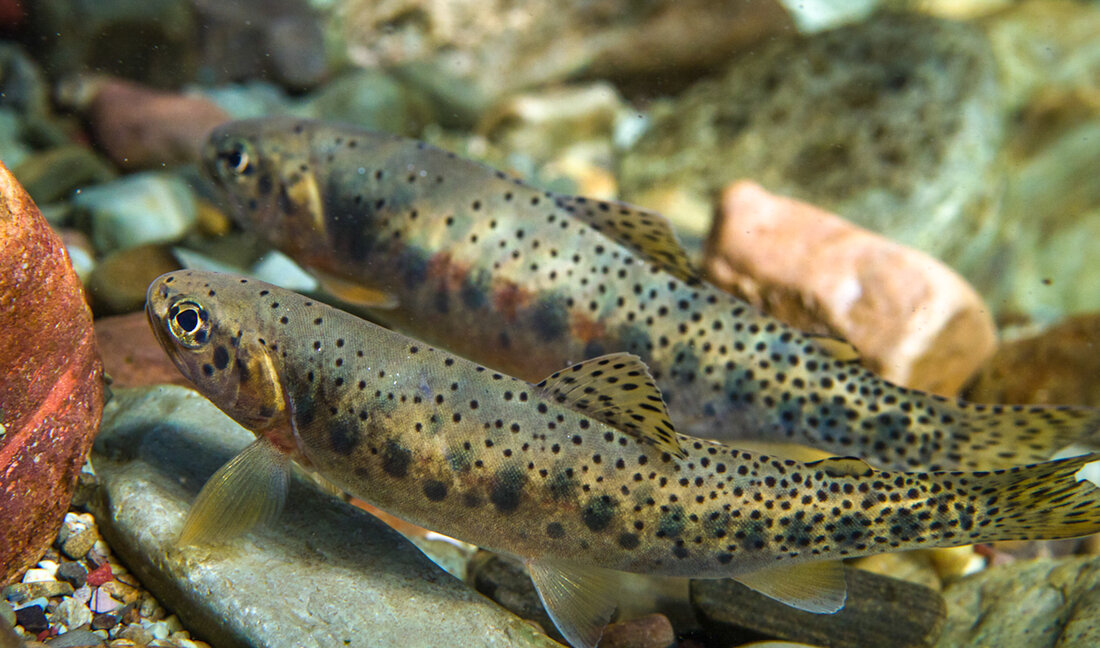
\includegraphics{trout.png}

This plan represents the culmination of a collaborative planning process
undertaken in the Elk River watershed over many months of work with a
multi-partner planning team of individuals and groups passionate about
the conservation and restoration of freshwater ecosystems and the
species they support. Plan development was funded by the BC Salmon
Restoration and Innovation Fund, the Canada Nature Fund for Aquatic
Species at Risk, and the RBC Bluewater Project. We were fortunate to
benefit from the feedback, guidance, and wisdom of many groups and
individuals who volunteered their time throughout this process --- this
publication would not have been possible without the engagement of our
partners and the planning team \href{project-partners.qmd}{see project
partners}.

We recognize the incredible fish passage and connectivity work that has
occurred in the Elk River watershed to date, and we are excited to
continue partnering with local groups and organizations to build up
existing initiatives and provide a road map to push connectivity
remediation forward over the next 20 years and beyond.

The Canadian Wildlife Federation recognizes that the lands and waters
that form the basis of this plan are the traditional unceded territory
of the Ktunaxa people. We are grateful for the opportunity to work to
benefit Westslope Cutthroat Trout (Oncorhynchus clarkii lewisi).

\bookmarksetup{startatroot}

\chapter*{Project Overview}\label{project-overview}
\addcontentsline{toc}{chapter}{Project Overview}

\markboth{Project Overview}{Project Overview}

\section*{Plan Purpose, Approach, and
Scope}\label{plan-purpose-approach-and-scope}
\addcontentsline{toc}{section}{Plan Purpose, Approach, and Scope}

\markright{Plan Purpose, Approach, and Scope}

The following Watershed Connectivity Remediation Plan (WCRP) represents
the culmination of a one-year collaborative planning effort for the Elk
River watershed, the overall aim of which is to reduce the threat of
aquatic barriers to resident, fluvial, and adfluvial fish and the
livelihoods that they support, including the continued sustenance,
cultural, and ceremonial needs of the Ktunaxa people both now and into
the future. This 30-year plan was developed to identify priority actions
that the Elk River WCRP planning team see
\href{project-partners.qmd}{Planning Team} for a list of team members
will undertake between 2021-2041 to conserve and restore fish passage in
the watershed through strategies aimed at barrier remediation and
barrier prevention.

WCRPs are long-term, actionable plans that blend local stakeholder and
rightsholder knowledge with innovative GIS analyses to gain a shared
understanding of where remediation efforts will have the greatest
benefit for fish. The planning process is inspired by the
\href{https://cmp-openstandards.org/wp-content/uploads/2020/07/CMP-Open-Standards-for-the-Practice-of-Conservation-v4.0.pdf}{Conservation
Standards} (v.4.0), which is a conservation planning framework that
allows planning teams to systematically identify, implement, and monitor
strategies to apply the most effective solutions to high-priority
conservation problems. There is a rich history of fish and fish habitat
conservation and restoration work in the Elk River watershed that this
WCRP builds upon, including the work undertaken by the Ktunaxa Nation,
the Province of British Columbia, and industry proponents, among others.
The Canadian Wildlife Federation will continue to engage and coordinate
with local partners and existing initiatives, including the
\href{https://www2.gov.bc.ca/gov/content/environment/natural-resource-stewardship/cumulative-effects-framework/regional-assessments/kootenay-boundary/elk-valley-cemf}{Elk
Valley Cumulative Effects Management Framework}, the Elk Valley Fish and
Fish Habitat Committee, and the
\href{https://elkrivercollaborative.ca/}{Elk River Watershed
Collaborative Monitoring Program}.

The planning team compiled existing barrier location and assessment
data, habitat data, and previously identified priorities, and combined
this with local knowledge to create a strategic watershed-scale plan to
improve connectivity. To expand on this work, the Elk River WCRP
planning team applied the WCRP planning framework to define the thematic
scope of freshwater connectivity and refine the geographic scope to
identify those portions of the watershed where barrier prioritization
will be conducted, and subsequent remediation efforts will take place.
Additionally, the team selected target fish species, assessed their
current connectivity status in the watershed, defined concrete goals for
gains in connectivity, and developed an intermediate list of barriers
for remediation to achieve those goals. Field assessments were completed
for 31 barriers above Elko Dam, and 21 barriers below Elko Dam on the
preliminary barrier list during the summer of 2021, followed by a series
of WCRP Update Workshops in winter 2021. The aim of these workshops was
for the team to receive updates on progress made during the field
season, review assessment results and identify priority barriers, revise
the connectivity status assessment and goals, and update the Operational
Plan for 2022. While the current version of this plan is based on the
best-available information at the time of publishing, WCRPs are intended
to be living plans that are updated regularly as new information becomes
available, or if local priorities and contexts change. As such, this
document should be interpreted as a current snap-shot in time, and
future iterations of this WCRP will build upon the material presented in
this plan to continuously improve aquatic barrier remediation for fish
in the Elk River watershed. For more information on how WCRPs are
developed, see Mazany-Wright, Noseworthy, et al. (2021).

\section*{Vision Statement}\label{vision-statement}
\addcontentsline{toc}{section}{Vision Statement}

\markright{Vision Statement}

Healthy, well-connected streams and rivers within the Elk River
watershed support thriving populations of Westslope Cutthroat Trout.
Watershed users work together to mitigate the negative impacts of
aquatic barriers, improving the resiliency of streams and rivers for the
benefit and appreciation of all.

\section*{Project Scope}\label{project-scope}
\addcontentsline{toc}{section}{Project Scope}

\markright{Project Scope}

Connectivity is a critical component of freshwater ecosystems that
encompasses a variety of factors related to ecosystem structure and
function, such as the ability of aquatic organisms to disperse and/or
migrate, the transportation of energy and matter (e.g., nutrient cycling
and sediment flows), and temperature regulation (Seliger and Zeiringer
(2018)). Though each of these factors are important when considering the
health of a watershed, for the purposes of this WCRP the term
``connectivity'' is defined as the degree to which aquatic organisms can
disperse and/or migrate freely through freshwater systems. Within this
context, connectivity is primarily constrained by physical barriers
including anthropogenic infrastructure such as dams, weirs, and stream
crossings, and natural features such as waterfalls and debris flows.
This plan is intended to focus on the direct remediation and prevention
of localized, physical barriers instead of the broad land-use patterns
that are causing chronic connectivity issues in the watershed. The
planning team decided that the primary focus of this WCRP is addressing
barriers to longitudinal connectivity (i.e., along the
upstream-downstream plane) due to the magnitude of the threat posed by
linear development (i.e., road and rail lines) in the watershed. In the
Elk River watershed, an additional connectivity consideration is
identifying barriers that should not be remediated to protect
genetically pure Westslope Cutthroat Trout (Oncorhunchus clarkii lewisi)
populations and mitigate the threat of introgression due to aquatic
invasive species (AIS).

\begin{figure}

\centering{

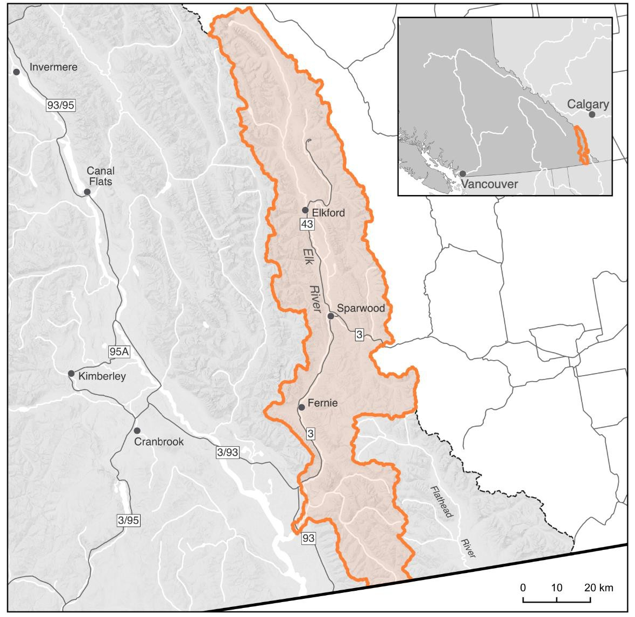
\includegraphics{content/images/geo-scope-elkr.png}

}

\caption{\label{fig-geoscope}The primary geographic scope --- the Elk
River watershed.}

\end{figure}%

The primary geographic scope of this WCRP is the Elk River watershed,
located in the Kootenays along the southeastern portion of the British
Columbia-Alberta border. The scope constitutes the Elk River ``watershed
group'' as defined by the
\href{https://catalogue.data.gov.bc.ca/dataset/freshwater-atlas-watershed-groups}{British
Columbia Freshwater Atlas (FWA)}, due to an effort made to standardize
spatial scales of the watershed groups. A consistent spatial framework
was necessary to undertake a watershed-selection process at the
provincial scale to identify target watersheds to improve connectivity
for salmonids. The Elk River watershed was identified by the BC Fish
Passage Restoration Initiative as one of four target watersheds for WCRP
development (Mazany-Wright, Norris, et al. (2021b)). The Elk River
watershed has a drainage area of 430,937 ha, spanning from the Rocky
Mountains in the northeast, the border with the United States in the
south, and the confluence with the Koocanusa Reservoir in the southwest
(Figure~\ref{fig-geoscope}).

\global\setlength{\Oldarrayrulewidth}{\arrayrulewidth}

\global\setlength{\Oldtabcolsep}{\tabcolsep}

\setlength{\tabcolsep}{2pt}

\renewcommand*{\arraystretch}{1.5}



\providecommand{\ascline}[3]{\noalign{\global\arrayrulewidth #1}\arrayrulecolor[HTML]{#2}\cline{#3}}

\begin{longtable}[c]{|p{1.36in}|p{1.43in}|p{2.15in}}

\caption{\label{tbl-targspec}Target fish species in the Elk River
watershed. The Secwepemctsín and Western common and scientific species
names are provided.}

\tabularnewline

\hhline{>{\arrayrulecolor[HTML]{666666}\global\arrayrulewidth=1.5pt}->{\arrayrulecolor[HTML]{666666}\global\arrayrulewidth=1.5pt}->{\arrayrulecolor[HTML]{666666}\global\arrayrulewidth=1.5pt}-}

\multicolumn{1}{>{\cellcolor[HTML]{008270}\raggedright}m{\dimexpr 1.36in+0\tabcolsep}}{\textcolor[HTML]{FFFFFF}{\fontsize{11}{11}\selectfont{\global\setmainfont{Arial}{Secwepemctsín}}}} & \multicolumn{1}{>{\cellcolor[HTML]{008270}\raggedright}m{\dimexpr 1.43in+0\tabcolsep}}{\textcolor[HTML]{FFFFFF}{\fontsize{11}{11}\selectfont{\global\setmainfont{Arial}{Common\ Name}}}} & \multicolumn{1}{>{\cellcolor[HTML]{008270}\raggedright}m{\dimexpr 2.15in+0\tabcolsep}}{\textcolor[HTML]{FFFFFF}{\fontsize{11}{11}\selectfont{\global\setmainfont{Arial}{Scientific\ Name}}}} \\

\noalign{\global\arrayrulewidth 0pt}\arrayrulecolor[HTML]{000000}

\hhline{>{\arrayrulecolor[HTML]{666666}\global\arrayrulewidth=1.5pt}->{\arrayrulecolor[HTML]{666666}\global\arrayrulewidth=1.5pt}->{\arrayrulecolor[HTML]{666666}\global\arrayrulewidth=1.5pt}-}\endfirsthead 

\hhline{>{\arrayrulecolor[HTML]{666666}\global\arrayrulewidth=1.5pt}->{\arrayrulecolor[HTML]{666666}\global\arrayrulewidth=1.5pt}->{\arrayrulecolor[HTML]{666666}\global\arrayrulewidth=1.5pt}-}

\multicolumn{1}{>{\cellcolor[HTML]{008270}\raggedright}m{\dimexpr 1.36in+0\tabcolsep}}{\textcolor[HTML]{FFFFFF}{\fontsize{11}{11}\selectfont{\global\setmainfont{Arial}{Secwepemctsín}}}} & \multicolumn{1}{>{\cellcolor[HTML]{008270}\raggedright}m{\dimexpr 1.43in+0\tabcolsep}}{\textcolor[HTML]{FFFFFF}{\fontsize{11}{11}\selectfont{\global\setmainfont{Arial}{Common\ Name}}}} & \multicolumn{1}{>{\cellcolor[HTML]{008270}\raggedright}m{\dimexpr 2.15in+0\tabcolsep}}{\textcolor[HTML]{FFFFFF}{\fontsize{11}{11}\selectfont{\global\setmainfont{Arial}{Scientific\ Name}}}} \\

\noalign{\global\arrayrulewidth 0pt}\arrayrulecolor[HTML]{000000}

\hhline{>{\arrayrulecolor[HTML]{666666}\global\arrayrulewidth=1.5pt}->{\arrayrulecolor[HTML]{666666}\global\arrayrulewidth=1.5pt}->{\arrayrulecolor[HTML]{666666}\global\arrayrulewidth=1.5pt}-}\endhead



\multicolumn{1}{>{\raggedright}m{\dimexpr 1.36in+0\tabcolsep}}{\textcolor[HTML]{000000}{\fontsize{11}{11}\selectfont{\global\setmainfont{Arial}{Kekèsu}}}} & \multicolumn{1}{>{\raggedright}m{\dimexpr 1.43in+0\tabcolsep}}{\textcolor[HTML]{000000}{\fontsize{11}{11}\selectfont{\global\setmainfont{Arial}{Chinook\ Salmon}}}} & \multicolumn{1}{>{\raggedright}m{\dimexpr 2.15in+0\tabcolsep}}{\textcolor[HTML]{000000}{\fontsize{11}{11}\selectfont{\global\setmainfont{Arial}{Oncorhynchus\ tshawytscha}}}} \\

\noalign{\global\arrayrulewidth 0pt}\arrayrulecolor[HTML]{000000}





\multicolumn{1}{>{\raggedright}m{\dimexpr 1.36in+0\tabcolsep}}{\textcolor[HTML]{000000}{\fontsize{11}{11}\selectfont{\global\setmainfont{Arial}{Sxeyqs}}}} & \multicolumn{1}{>{\raggedright}m{\dimexpr 1.43in+0\tabcolsep}}{\textcolor[HTML]{000000}{\fontsize{11}{11}\selectfont{\global\setmainfont{Arial}{Coho\ Salmon}}}} & \multicolumn{1}{>{\raggedright}m{\dimexpr 2.15in+0\tabcolsep}}{\textcolor[HTML]{000000}{\fontsize{11}{11}\selectfont{\global\setmainfont{Arial}{Oncorhynchus\ kisutch}}}} \\

\noalign{\global\arrayrulewidth 0pt}\arrayrulecolor[HTML]{000000}





\multicolumn{1}{>{\raggedright}m{\dimexpr 1.36in+0\tabcolsep}}{\textcolor[HTML]{000000}{\fontsize{11}{11}\selectfont{\global\setmainfont{Arial}{Sqlelten7ùwi}}}} & \multicolumn{1}{>{\raggedright}m{\dimexpr 1.43in+0\tabcolsep}}{\textcolor[HTML]{000000}{\fontsize{11}{11}\selectfont{\global\setmainfont{Arial}{Sockeye\ Salmon}}}} & \multicolumn{1}{>{\raggedright}m{\dimexpr 2.15in+0\tabcolsep}}{\textcolor[HTML]{000000}{\fontsize{11}{11}\selectfont{\global\setmainfont{Arial}{Oncorhynchus\ nerka}}}} \\

\noalign{\global\arrayrulewidth 0pt}\arrayrulecolor[HTML]{000000}

\hhline{>{\arrayrulecolor[HTML]{666666}\global\arrayrulewidth=1.5pt}->{\arrayrulecolor[HTML]{666666}\global\arrayrulewidth=1.5pt}->{\arrayrulecolor[HTML]{666666}\global\arrayrulewidth=1.5pt}-}


\end{longtable}

\arrayrulecolor[HTML]{000000}

\global\setlength{\arrayrulewidth}{\Oldarrayrulewidth}

\global\setlength{\tabcolsep}{\Oldtabcolsep}

\renewcommand*{\arraystretch}{1}

The Elk River watershed comprises part of the traditional territory of
the Ktunaxa peoples, and contains culturally and economically important
populations of Westslope Cutthroat Trout, which historically supported
Indigenous sustenance and trading economies. The geographic scope for
this WCRP was further refined by the planning team through the exclusion
of the Flathead River system from the defined watershed group. The
Flathead River is hydrographically and topographically distinct from the
rest of the watershed and does not flow into the Elk River and Columbia
River systems, but is considered part of the watershed group in the FWA.
The planning team decided that the watershed connectivity planning
process should focus on just the Elk River system and the important
Westslope Cutthroat Trout populations supported by the streams and
rivers there.

Additionally, the planning team decided to divide the remaining
watershed into two discrete WCRP units--- 1) Upstream of the Elko Dam
and 2) Downstream of the Elko Dam. The Elko Dam was constructed in 1924
on the site of a series of waterfalls that were natural barriers to
upstream fish passage, and the dam facility remains impassable to all
fish species (J. Bisset, Bisset \& Associates, pers. comm., Ladell and
Baxter (n.d.)). The Elko Dam plays an important role in preventing the
upstream dispersal of invasive/hybridized trout populations from the
Columbia River thereby acting as an important barrier to introgression
(Lamson (2018)). This role, coupled with the waterfalls acting as
natural barrier prior to dam construction, provided the justification to
remove the Elko Dam from consideration as a barrier to remediate. Each
WCRP unit has Westslope Cutthroat Trout populations with unique
life-history forms, and was evaluated independently for connectivity
status assessments, goal setting, and barrier prioritization analyses.

Finally, ``potentially accessible'' stream segments, which are defined
as streams that Westslope Cutthroat Trout should be able to access in
the absence of anthropogenic barriers, were modelled to set constraints
on the geographic scope (Figure~\ref{fig-strseg}). Potentially
accessible stream segments were spatially delineated using Westslope
Cutthroat Trout observation and distribution data, as well as data on
``exclusionary points'', which are waterfalls greater than 5 m in height
and gradient barriers where the stream slope exceeds 30\% (only in cases
where no known populations or observations exist upstream of these
points). These maps were explored by the planning team to incorporate
additional local knowledge, ensure accuracy, and finalize the
constraints on potentially accessible stream segments. All stream
segments not identified as potentially accessible were removed from the
scope for further consideration. The resulting constrained geographic
scope formed the foundation for all subsequent analyses and planning
steps, including mapping and modelling useable habitat types,
quantifying the current connectivity status, goal setting, and action
planning (Mazany-Wright, Norris, et al. (2021a)).

\begin{figure}

\centering{

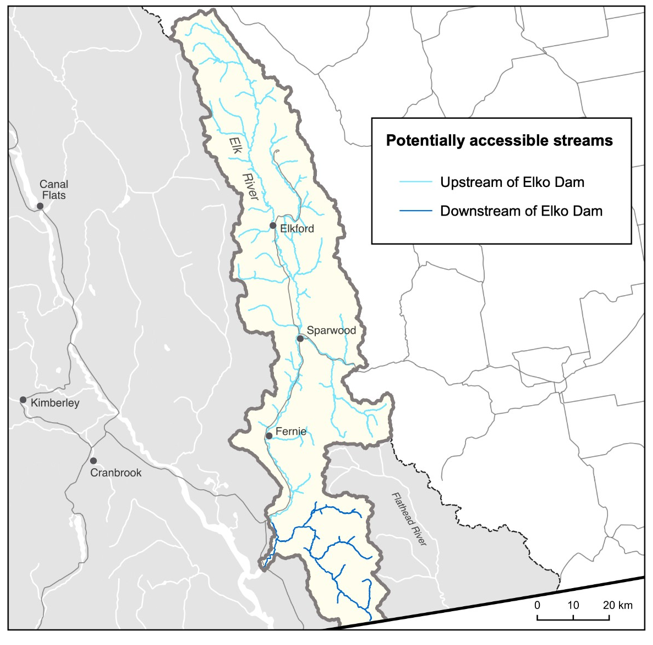
\includegraphics{content/images/accessible-streams-elkr.png}

}

\caption{\label{fig-strseg}Potentially accessible stream segments within
the Upstream of the Elko Dam (light blue) and Downstream of the Elko Dam
(dark blue) units in Elk River watershed. These do not represent useable
habitat types, but rather identifies the stream segments within which
habitat modelling and barrier mapping and prioritization was
undertaken.}

\end{figure}%

\section*{Target species}\label{target-species}
\addcontentsline{toc}{section}{Target species}

\markright{Target species}

Target species represent the ecologically and culturally important
species for which habitat connectivity is being conserved and/or
restored in the watershed. In the Elk River watershed, the planning team
selected Westslope Cutthroat Trout as the target species. The selection
of this target species was driven primarily by the target species of the
primary fund supporting this planning work. The planning team also
identified other culturally and ecologically important species within
the watershed to consider for inclusion in future iterations of the
WCRP, including Burbot (Lota lota), Bull Trout (Salvelinus confluentus),
and Whitefish (Prosopium williamsoni).

\subsection*{Westslope Cutthroat Trout \textbar{} Oncorhynchus clarkii
lewisi}\label{westslope-cutthroat-trout-oncorhynchus-clarkii-lewisi}
\addcontentsline{toc}{subsection}{Westslope Cutthroat Trout \textbar{}
Oncorhynchus clarkii lewisi}

Westslope Cutthroat Trout is a cultural and ecological keystone species
in the Elk River watershed, playing an important role in structuring
aquatic ecosystems and contributing to nutrient recovery for riparian
vegetation and forests in cold water streams and lakes, including small,
steep streams not accessible to other fish species (Willson and Halupka
(1995), COSEWIC (2016)). Westslope Cutthroat Trout are a traditionally
important species for the Ktunaxa people and provide substantial
economic value for recreational and commercial fisheries. Westslope
Cutthroat Trout populations have declined in recent decades due to a
combination of threats including, introgressive hybridization with AIS
(particularly Rainbow Trout; Oncorhynchus mykiss), habitat degradation,
fragmentation, overexploitation, and rising water temperatures due to
climate change (COSEWIC (2016), Lamson (2018)). Most relevant to this
WCRP, road networks have disrupted many parts of the Elk River watershed
thereby increasing the density of stream crossings, leading to stream
fragmentation and limiting upstream fish passage. Additionally, some
entire headwater reaches have been disrupted or have disappeared due to
rock drains associated with mining activity in the watershed (COSEWIC
(2016)).

\global\setlength{\Oldarrayrulewidth}{\arrayrulewidth}

\global\setlength{\Oldtabcolsep}{\tabcolsep}

\setlength{\tabcolsep}{2pt}

\renewcommand*{\arraystretch}{1.5}



\providecommand{\ascline}[3]{\noalign{\global\arrayrulewidth #1}\arrayrulecolor[HTML]{#2}\cline{#3}}

\begin{longtable}[c]{|p{2.14in}|p{1.37in}|p{0.91in}|p{1.50in}}

\caption{\label{tbl-wctrout}Westslope Cutthroat Trout Pacific
populations Designated Unit assessment. Assessments undertaken by the
Committee on the Status of Endangered Wildlife in Canada (2016).}

\tabularnewline

\hhline{>{\arrayrulecolor[HTML]{666666}\global\arrayrulewidth=1.5pt}->{\arrayrulecolor[HTML]{666666}\global\arrayrulewidth=1.5pt}->{\arrayrulecolor[HTML]{666666}\global\arrayrulewidth=1.5pt}->{\arrayrulecolor[HTML]{666666}\global\arrayrulewidth=1.5pt}-}

\multicolumn{1}{>{\cellcolor[HTML]{008270}\raggedright}m{\dimexpr 2.14in+0\tabcolsep}}{\textcolor[HTML]{FFFFFF}{\fontsize{11}{11}\selectfont{\global\setmainfont{Arial}{COSEWIC\ Designated\ Unit}}}} & \multicolumn{1}{>{\cellcolor[HTML]{008270}\raggedright}m{\dimexpr 1.37in+0\tabcolsep}}{\textcolor[HTML]{FFFFFF}{\fontsize{11}{11}\selectfont{\global\setmainfont{Arial}{Status}}}} & \multicolumn{1}{>{\cellcolor[HTML]{008270}\raggedright}m{\dimexpr 0.91in+0\tabcolsep}}{\textcolor[HTML]{FFFFFF}{\fontsize{11}{11}\selectfont{\global\setmainfont{Arial}{Trend}}}} & \multicolumn{1}{>{\cellcolor[HTML]{008270}\raggedright}m{\dimexpr 1.5in+0\tabcolsep}}{\textcolor[HTML]{FFFFFF}{\fontsize{11}{11}\selectfont{\global\setmainfont{Arial}{Generation\ length}}}} \\

\noalign{\global\arrayrulewidth 0pt}\arrayrulecolor[HTML]{000000}

\hhline{>{\arrayrulecolor[HTML]{666666}\global\arrayrulewidth=1.5pt}->{\arrayrulecolor[HTML]{666666}\global\arrayrulewidth=1.5pt}->{\arrayrulecolor[HTML]{666666}\global\arrayrulewidth=1.5pt}->{\arrayrulecolor[HTML]{666666}\global\arrayrulewidth=1.5pt}-}\endfirsthead 

\hhline{>{\arrayrulecolor[HTML]{666666}\global\arrayrulewidth=1.5pt}->{\arrayrulecolor[HTML]{666666}\global\arrayrulewidth=1.5pt}->{\arrayrulecolor[HTML]{666666}\global\arrayrulewidth=1.5pt}->{\arrayrulecolor[HTML]{666666}\global\arrayrulewidth=1.5pt}-}

\multicolumn{1}{>{\cellcolor[HTML]{008270}\raggedright}m{\dimexpr 2.14in+0\tabcolsep}}{\textcolor[HTML]{FFFFFF}{\fontsize{11}{11}\selectfont{\global\setmainfont{Arial}{COSEWIC\ Designated\ Unit}}}} & \multicolumn{1}{>{\cellcolor[HTML]{008270}\raggedright}m{\dimexpr 1.37in+0\tabcolsep}}{\textcolor[HTML]{FFFFFF}{\fontsize{11}{11}\selectfont{\global\setmainfont{Arial}{Status}}}} & \multicolumn{1}{>{\cellcolor[HTML]{008270}\raggedright}m{\dimexpr 0.91in+0\tabcolsep}}{\textcolor[HTML]{FFFFFF}{\fontsize{11}{11}\selectfont{\global\setmainfont{Arial}{Trend}}}} & \multicolumn{1}{>{\cellcolor[HTML]{008270}\raggedright}m{\dimexpr 1.5in+0\tabcolsep}}{\textcolor[HTML]{FFFFFF}{\fontsize{11}{11}\selectfont{\global\setmainfont{Arial}{Generation\ length}}}} \\

\noalign{\global\arrayrulewidth 0pt}\arrayrulecolor[HTML]{000000}

\hhline{>{\arrayrulecolor[HTML]{666666}\global\arrayrulewidth=1.5pt}->{\arrayrulecolor[HTML]{666666}\global\arrayrulewidth=1.5pt}->{\arrayrulecolor[HTML]{666666}\global\arrayrulewidth=1.5pt}->{\arrayrulecolor[HTML]{666666}\global\arrayrulewidth=1.5pt}-}\endhead



\multicolumn{1}{>{\raggedright}m{\dimexpr 2.14in+0\tabcolsep}}{\textcolor[HTML]{000000}{\fontsize{11}{11}\selectfont{\global\setmainfont{Arial}{Pacific\ populations}}}} & \multicolumn{1}{>{\raggedright}m{\dimexpr 1.37in+0\tabcolsep}}{\textcolor[HTML]{000000}{\fontsize{11}{11}\selectfont{\global\setmainfont{Arial}{Special\ concern}}}} & \multicolumn{1}{>{\raggedright}m{\dimexpr 0.91in+0\tabcolsep}}{\textcolor[HTML]{000000}{\fontsize{11}{11}\selectfont{\global\setmainfont{Arial}{Declining}}}} & \multicolumn{1}{>{\raggedright}m{\dimexpr 1.5in+0\tabcolsep}}{\textcolor[HTML]{000000}{\fontsize{11}{11}\selectfont{\global\setmainfont{Arial}{4-8\ years}}}} \\

\noalign{\global\arrayrulewidth 0pt}\arrayrulecolor[HTML]{000000}

\hhline{>{\arrayrulecolor[HTML]{666666}\global\arrayrulewidth=1.5pt}->{\arrayrulecolor[HTML]{666666}\global\arrayrulewidth=1.5pt}->{\arrayrulecolor[HTML]{666666}\global\arrayrulewidth=1.5pt}->{\arrayrulecolor[HTML]{666666}\global\arrayrulewidth=1.5pt}-}


\end{longtable}

\arrayrulecolor[HTML]{000000}

\global\setlength{\arrayrulewidth}{\Oldarrayrulewidth}

\global\setlength{\tabcolsep}{\Oldtabcolsep}

\renewcommand*{\arraystretch}{1}

Westslope Cutthroat Trout populations and subpopulations found in the
Elk River watershed are captured by the ``Pacific populations''
Designated Unit as defined by the Committee on the Status of Endangered
Wildlife in Canada (COSEWIC), which has a core distribution covering the
upper Kootenay River drainage (Table~\ref{tbl-wctrout}). Specifically,
the Elk River watershed contains the Elk River and Upper Kootenay
population groups, with each population group containing multiple
sub-populations with variable life history forms
(Table~\ref{tbl-wcrp-pop}). High levels of hybridization exist in most
waterbodies connected to the Koocanusa Reservoir (i.e., the Upper
Kootenay population group), including the Elk River mainstem downstream
of the Elko Dam and much of the Wigwam and Lodgepole systems. Generally,
the hybridization levels upstream of Elko Dam are quite low, though
there is known hybridization occurring in the Michel Creek sub-drainage
(COSEWIC (2016); H. Lamson, BC Ministry of Environment pers. comm.).
Pure Westslope Cutthroat Trout sub-populations exist in the upper
Fording River (upstream of Josephine Falls), Greenhills Creek, Forsyth
Creek, Grave Creek, Harmer Creek, Morrissey Creek, Weary Creek, upper
Lodgepole Creek, and the upper Elk River (Lamson (2018)).

\global\setlength{\Oldarrayrulewidth}{\arrayrulewidth}

\global\setlength{\Oldtabcolsep}{\tabcolsep}

\setlength{\tabcolsep}{2pt}

\renewcommand*{\arraystretch}{1.5}



\providecommand{\ascline}[3]{\noalign{\global\arrayrulewidth #1}\arrayrulecolor[HTML]{#2}\cline{#3}}

\begin{longtable}[c]{|p{2.27in}|p{1.47in}|p{8.11in}|p{2.78in}|p{1.82in}}

\caption{\label{tbl-wcrp-pop}Population group details for each WCRP Unit
- Upstream and Downstream of the Elko Dam - in the Elk River watershed
(COSEWIC 2016, Lamson 2018).}

\tabularnewline

\hhline{>{\arrayrulecolor[HTML]{666666}\global\arrayrulewidth=1.5pt}->{\arrayrulecolor[HTML]{666666}\global\arrayrulewidth=1.5pt}->{\arrayrulecolor[HTML]{666666}\global\arrayrulewidth=1.5pt}->{\arrayrulecolor[HTML]{666666}\global\arrayrulewidth=1.5pt}->{\arrayrulecolor[HTML]{666666}\global\arrayrulewidth=1.5pt}-}

\multicolumn{1}{>{\cellcolor[HTML]{008270}\raggedright}m{\dimexpr 2.27in+0\tabcolsep}}{\textcolor[HTML]{FFFFFF}{\fontsize{11}{11}\selectfont{\global\setmainfont{Arial}{WCRP\ Unit}}}} & \multicolumn{1}{>{\cellcolor[HTML]{008270}\raggedright}m{\dimexpr 1.47in+0\tabcolsep}}{\textcolor[HTML]{FFFFFF}{\fontsize{11}{11}\selectfont{\global\setmainfont{Arial}{Population\ Group}}}} & \multicolumn{1}{>{\cellcolor[HTML]{008270}\raggedright}m{\dimexpr 8.11in+0\tabcolsep}}{\textcolor[HTML]{FFFFFF}{\fontsize{11}{11}\selectfont{\global\setmainfont{Arial}{Waterbodies}}}} & \multicolumn{1}{>{\cellcolor[HTML]{008270}\raggedright}m{\dimexpr 2.78in+0\tabcolsep}}{\textcolor[HTML]{FFFFFF}{\fontsize{11}{11}\selectfont{\global\setmainfont{Arial}{Life\ History\ Forms}}}} & \multicolumn{1}{>{\cellcolor[HTML]{008270}\raggedright}m{\dimexpr 1.82in+0\tabcolsep}}{\textcolor[HTML]{FFFFFF}{\fontsize{11}{11}\selectfont{\global\setmainfont{Arial}{Threat\ of\ Hybridization}}}} \\

\noalign{\global\arrayrulewidth 0pt}\arrayrulecolor[HTML]{000000}

\hhline{>{\arrayrulecolor[HTML]{666666}\global\arrayrulewidth=1.5pt}->{\arrayrulecolor[HTML]{666666}\global\arrayrulewidth=1.5pt}->{\arrayrulecolor[HTML]{666666}\global\arrayrulewidth=1.5pt}->{\arrayrulecolor[HTML]{666666}\global\arrayrulewidth=1.5pt}->{\arrayrulecolor[HTML]{666666}\global\arrayrulewidth=1.5pt}-}\endfirsthead 

\hhline{>{\arrayrulecolor[HTML]{666666}\global\arrayrulewidth=1.5pt}->{\arrayrulecolor[HTML]{666666}\global\arrayrulewidth=1.5pt}->{\arrayrulecolor[HTML]{666666}\global\arrayrulewidth=1.5pt}->{\arrayrulecolor[HTML]{666666}\global\arrayrulewidth=1.5pt}->{\arrayrulecolor[HTML]{666666}\global\arrayrulewidth=1.5pt}-}

\multicolumn{1}{>{\cellcolor[HTML]{008270}\raggedright}m{\dimexpr 2.27in+0\tabcolsep}}{\textcolor[HTML]{FFFFFF}{\fontsize{11}{11}\selectfont{\global\setmainfont{Arial}{WCRP\ Unit}}}} & \multicolumn{1}{>{\cellcolor[HTML]{008270}\raggedright}m{\dimexpr 1.47in+0\tabcolsep}}{\textcolor[HTML]{FFFFFF}{\fontsize{11}{11}\selectfont{\global\setmainfont{Arial}{Population\ Group}}}} & \multicolumn{1}{>{\cellcolor[HTML]{008270}\raggedright}m{\dimexpr 8.11in+0\tabcolsep}}{\textcolor[HTML]{FFFFFF}{\fontsize{11}{11}\selectfont{\global\setmainfont{Arial}{Waterbodies}}}} & \multicolumn{1}{>{\cellcolor[HTML]{008270}\raggedright}m{\dimexpr 2.78in+0\tabcolsep}}{\textcolor[HTML]{FFFFFF}{\fontsize{11}{11}\selectfont{\global\setmainfont{Arial}{Life\ History\ Forms}}}} & \multicolumn{1}{>{\cellcolor[HTML]{008270}\raggedright}m{\dimexpr 1.82in+0\tabcolsep}}{\textcolor[HTML]{FFFFFF}{\fontsize{11}{11}\selectfont{\global\setmainfont{Arial}{Threat\ of\ Hybridization}}}} \\

\noalign{\global\arrayrulewidth 0pt}\arrayrulecolor[HTML]{000000}

\hhline{>{\arrayrulecolor[HTML]{666666}\global\arrayrulewidth=1.5pt}->{\arrayrulecolor[HTML]{666666}\global\arrayrulewidth=1.5pt}->{\arrayrulecolor[HTML]{666666}\global\arrayrulewidth=1.5pt}->{\arrayrulecolor[HTML]{666666}\global\arrayrulewidth=1.5pt}->{\arrayrulecolor[HTML]{666666}\global\arrayrulewidth=1.5pt}-}\endhead



\multicolumn{1}{>{\raggedright}m{\dimexpr 2.27in+0\tabcolsep}}{\textcolor[HTML]{000000}{\fontsize{11}{11}\selectfont{\global\setmainfont{Arial}{Upstream\ of\ the\ Elko\ Dam}}}} & \multicolumn{1}{>{\raggedright}m{\dimexpr 1.47in+0\tabcolsep}}{\textcolor[HTML]{000000}{\fontsize{11}{11}\selectfont{\global\setmainfont{Arial}{Elk\ River}}}} & \multicolumn{1}{>{\raggedright}m{\dimexpr 8.11in+0\tabcolsep}}{\textcolor[HTML]{000000}{\fontsize{11}{11}\selectfont{\global\setmainfont{Arial}{Elk\ River\ mainstem\ and\ all\ tributaries\ above\ Elko\ Dam}}}} & \multicolumn{1}{>{\raggedright}m{\dimexpr 2.78in+0\tabcolsep}}{\textcolor[HTML]{000000}{\fontsize{11}{11}\selectfont{\global\setmainfont{Arial}{Stream-resident\ and\ fluvial}}}} & \multicolumn{1}{>{\raggedright}m{\dimexpr 1.82in+0\tabcolsep}}{\textcolor[HTML]{000000}{\fontsize{11}{11}\selectfont{\global\setmainfont{Arial}{Low}}}} \\

\noalign{\global\arrayrulewidth 0pt}\arrayrulecolor[HTML]{000000}





\multicolumn{1}{>{\raggedright}m{\dimexpr 2.27in+0\tabcolsep}}{\textcolor[HTML]{000000}{\fontsize{11}{11}\selectfont{\global\setmainfont{Arial}{Downstream\ of\ the\ Elko\ Dam}}}} & \multicolumn{1}{>{\raggedright}m{\dimexpr 1.47in+0\tabcolsep}}{\textcolor[HTML]{000000}{\fontsize{11}{11}\selectfont{\global\setmainfont{Arial}{Upper\ Kootenay}}}} & \multicolumn{1}{>{\raggedright}m{\dimexpr 8.11in+0\tabcolsep}}{\textcolor[HTML]{000000}{\fontsize{11}{11}\selectfont{\global\setmainfont{Arial}{Elk\ River\ mainstem\ below\ Elko\ Dam\ and\ Wigwam\ and\ Lodgepole\ systems\ (connected\ to\ the\ Koocanusa\ Reservoir)}}}} & \multicolumn{1}{>{\raggedright}m{\dimexpr 2.78in+0\tabcolsep}}{\textcolor[HTML]{000000}{\fontsize{11}{11}\selectfont{\global\setmainfont{Arial}{Stream\ resident,\ fluvial,\ and\ adfluvial}}}} & \multicolumn{1}{>{\raggedright}m{\dimexpr 1.82in+0\tabcolsep}}{\textcolor[HTML]{000000}{\fontsize{11}{11}\selectfont{\global\setmainfont{Arial}{High}}}} \\

\noalign{\global\arrayrulewidth 0pt}\arrayrulecolor[HTML]{000000}

\hhline{>{\arrayrulecolor[HTML]{666666}\global\arrayrulewidth=1.5pt}->{\arrayrulecolor[HTML]{666666}\global\arrayrulewidth=1.5pt}->{\arrayrulecolor[HTML]{666666}\global\arrayrulewidth=1.5pt}->{\arrayrulecolor[HTML]{666666}\global\arrayrulewidth=1.5pt}->{\arrayrulecolor[HTML]{666666}\global\arrayrulewidth=1.5pt}-}


\end{longtable}

\arrayrulecolor[HTML]{000000}

\global\setlength{\arrayrulewidth}{\Oldarrayrulewidth}

\global\setlength{\tabcolsep}{\Oldtabcolsep}

\renewcommand*{\arraystretch}{1}

Adult Westslope Cutthroat Trout overwinter in deep pools or lakes and
then generally move upstream to spawning habitat during high spring
flows, with spawning peaking between May and June. Fry emergence occurs
between July and August, with individuals migrating to lower velocity
rearing habitats in and around natal streams (COSEWIC (2016), ERA
(n.d.)). Westslope Cutthroat Trout exist with three distinct life
history forms in the Elk River watershed (Oliver (2009), ERA (n.d.)):

\begin{itemize}
\item
  Stream-resident --- individuals spend their entire life history within
  a restricted distribution of headwater streams, often because movement
  is restricted by natural barriers.
\item
  Fluvial --- individuals migrate between tributaries and larger
  mainstem rivers to complete various life-history stages (e.g.,
  spawning, overwintering).
\item
  Adfluvial --- individuals migrate between tributaries and
  lakes/reservoirs to complete life-history stages. See Appendix A for
  maps of modelled Westslope Cutthroat Trout habitat in the Elk River
  watershed.
\end{itemize}

\section*{Barrier Types}\label{barrier-types}
\addcontentsline{toc}{section}{Barrier Types}

\markright{Barrier Types}

The following table highlights which barrier types pose the greatest
threat to Westslope Cutthroat Trout in the watershed. The results of
this assessment were used to inform the subsequent planning steps, as
well as to identify knowledge gaps where there are little spatial data
to inform the assessment for a specific barrier type.

\begin{longtable}[]{@{}lllll@{}}

\caption{\label{tbl-barriertype}Barrier types in the Elk River watershed
and barrier rating assessment results. For each barrier type listed,
`Extent' refers to the proportion of Westslope Cutthroat Trout habitat
that is being blocked by that barrier type, `Severity' is the proportion
of structures for each barrier type that are known to block passage for
target species based on field assessments, and `Irreversibility' is the
degree to which the effects of a barrier type can be reversed and
connectivity restored.}

\tabularnewline

\caption{}\label{T_e94ee}\tabularnewline
\toprule\noalign{}
Barrier Types & Extent & Severity & Irreversibility & Overall Threat
Rating: \\
\midrule\noalign{}
\endfirsthead
\toprule\noalign{}
Barrier Types & Extent & Severity & Irreversibility & Overall Threat
Rating: \\
\midrule\noalign{}
\endhead
\bottomrule\noalign{}
\endlastfoot
Dams & Medium & Low & High & Low \\
Road-Stream Crossings & High & Low & Medium & High \\
Rail-stream Crossings & Low & High & High & Medium \\
Trail-stream Crossings & Low & Low & Low & Low \\
Lateral Barriers & Low & Low & High & Low \\
Sediment Wedges & Low & Low & Medium & Low \\
Landslides & Low & Low & High & Low \\

\end{longtable}

\subsection*{Dams}\label{dams}
\addcontentsline{toc}{subsection}{Dams}

There are 9 mapped dams on potential habitat in the watershed,
blocking698.19 km (39.83\% of the total blocked habitat) of modelled
spawning and rearing habitat, resulting in a Low extent. The Elko Dam is
excluded from this assessment due to its function in preventing
introgression and the spread of AIS upstream, and the historic natural
barrier at this site. The extent rating of these structures was
confirmed by the planning team --- there are a small number of known
dams in the watershed, mostly associated with mining activity (e.g.,
settling/tailing ponds). The Harmer Creek Dam was identified by the
planning team as an important dam to remediate to benefit a genetically
pure Westslope Cutthroat Trout population in the Grave-Harmer system,
and Teck Resources Ltd.~is currently undertaking an assessment process
to evaluate potential remediation options (W. Franklin, Teck Resources
Ltd., pers. comm.). There are no known fishways in the watershed, and
the identified dams likely block passage for Westslope Cutthroat Trout.
Due to the significant resources required to remediate dams and the Low
extent of dams in the watershed, a final pressure rating of Low was
assigned.

\subsection*{Road-stream Crossings}\label{road-stream-crossings}
\addcontentsline{toc}{subsection}{Road-stream Crossings}

Road-stream crossings are the most abundant barrier type in the
watershed, with 18 assessed and modelled crossings located on potential
habitat. Demographic road crossings (highways, municipal, and paved
roads) block 56.38 km of habitat (\textasciitilde40\% of the total
blocked habitat), with 0\% of assessed crossings having been identified
as barriers to fish passage. Resource roads potentially block 698.19 km
of habitat (\textasciitilde40\%), with 0\% of assessed crossings have
been identified as barriers. Significant land use and linear development
throughout the valley bottom, including Highways 3 and 43, have
disconnected the Elk River from important habitat in many tributaries.
The resource road-stream crossings are primarily associated with mining
and forestry activities in the watershed. The collective experience and
input from the planning team resulted in a Medium irreversibility rating
due to the technical complexity and resources required to remediate
road-stream crossings, though it was noted that this differs
considerably between resource roads and highway crossings.

\subsection*{Rail-stream crossings}\label{rail-stream-crossings}
\addcontentsline{toc}{subsection}{Rail-stream crossings}

There are relatively few rail-stream crossings in the watershed (65
crossings on potential habitat), potentially blocking only 13.99 km of
habitat (\textasciitilde3\% of the total habitat blocked). Only 14
rail-stream crossings have been assessed in the watershed, and of these
45\% are considered to be barriers. All rail- stream crossings in the
watershed are associated with the Canadian Pacific (CP) rail lines
running along the Elk River, Fording River, and Michel Creek. With
significant financial costs, technical challenges, and stakeholder
engagement required with CP to remediate these barriers, the planning
team decided on an overall pressure rating of Medium for this barrier
type.

\subsection*{Trail-stream crossings}\label{trail-stream-crossings}
\addcontentsline{toc}{subsection}{Trail-stream crossings}

There are very little spatial data available on trail-stream crossings
in the watershed, so the planning team was unable to numerically
quantify the Extent and Severity of this barrier type. The planning team
felt that recreational trail network crossings rarely significantly
block passage for Westslope Cutthroat Trout. Given that most crossings
will likely be fords or similar structures, the remediation costs
associated with these barriers would be quite low. Overall, the planning
team felt that the pressure rating for trail-stream crossings was likely
Low.

\subsection*{Lateral Barriers}\label{lateral-barriers}
\addcontentsline{toc}{subsection}{Lateral Barriers}

There are numerous types of lateral barriers that potentially occur in
the watershed, including dykes, berms, and linear development (i.e.,
road and rail lines), all of which can restrict the ability of Westslope
Cutthroat Trout to move into floodplains, riparian wetlands, and other
off-channel habitats. No comprehensive lateral barrier data exist within
the watershed, so pressure ratings were based on qualitative local
knowledge. Lateral barriers are not thought to be as prevalent as road-
or rail-stream crossings and are likely to be passable for at least
certain parts of the year where they do exist. Highway 3, Highway 43,
and the CP rail line were identified as potential lateral barriers that
disconnect the mainstem channels from their historic floodplain and
off-channel habitat. Overall, the planning team decided that a Low
pressure rating adequately captured the effect that lateral barriers are
having on connectivity in the watershed, while recognizing that the lack
of data on lateral barriers in the watershed is an important knowledge
gap to fill.

\subsection*{Sediment Wedges}\label{sediment-wedges}
\addcontentsline{toc}{subsection}{Sediment Wedges}

Sediment wedges include both mass wasting events and chronic bank
erosion that can lead to the deposition of sediment to such an extent as
to limit fish passage. The extent and severity of sediment wedges acting
as barriers fluctuates seasonally and annually due to natural and
human-induced changes to the flow regime, and natural barriers of this
type are difficult to include in a spatial prioritization framework due
to their transient nature. Both current and historic land-use practices,
including mining and forest-harvesting impacts, contribute to the
formation of sediment wedges in the watershed; however, the planning
team felt that the extent and severity were Low overall.

\subsection*{Landslides}\label{landslides}
\addcontentsline{toc}{subsection}{Landslides}

Though a relatively rare occurrence, landslides that result in
impediments to fish passage do occur in the watershed and can be
technically and financially difficult to remediate when they occur.
Overall, the planning team felt that a Low rating adequately captured
the effects of landslides, but felt that it was an important barrier
type to identify in this WCRP.

\bookmarksetup{startatroot}

\chapter*{Connectivity Status Assessment and
Goals}\label{connectivity-status-assessment-and-goals}
\addcontentsline{toc}{chapter}{Connectivity Status Assessment and Goals}

\markboth{Connectivity Status Assessment and Goals}{Connectivity Status
Assessment and Goals}

\section*{Connectivity Status
Assessment}\label{connectivity-status-assessment}
\addcontentsline{toc}{section}{Connectivity Status Assessment}

\markright{Connectivity Status Assessment}

The planning team devised two Key Ecological Attributes (KEAs) and
associated indicators to assess the current connectivity status of the
watershed -- Accessible habitat above Elko Dam and Accessible habitat
below Elko Dam (Table~\ref{tbl-connectivity}). KEAs are the key aspects
of Westslope Cutthroat Trout ecology that are being targeted by this
WCRP. The connectivity statuses for the Westslope Cutthroat Trout KEAs
were used to establish goals to improve habitat connectivity in the
watershed and will be the baseline against which progress is tracked
over time.

The current connectivity status assessment relies on GIS analyses to map
known and modelled barriers to fish passage, identify stream reaches
that have potential spawning and rearing habitat, estimate the
proportion of habitat that is currently accessible to target species,
and prioritize barriers for field assessment that would provide the
greatest gains in connectivity. For the connectivity status assessments
and barrier prioritization analysis the amount of spawning and rearing
habitat is aggregated without duplication (i.e., a stream segment is
only counted once if it is classified as both spawning and rearing
habitat; see \href{data-methods.qmd}{data methods}). To support a
flexible prioritization framework to identify priority barriers in the
watershed, two assumptions are made: 1) any modelled (i.e., the
passability status is unknown) or partial barriers are treated as
complete barriers to passage and 2) the habitat modelling is binary, it
does not assign any habitat quality values. As such, the current
connectivity status will be refined over time as more data on habitat
and barriers are collected. For more detail on how the connectivity
status assessments were conducted, see \href{data-methods.qmd}{data
methods}.

\begin{longtable}[]{@{}lllllll@{}}

\caption{\label{tbl-connectivity}Connectivity status assessment for (a)
habitat upstream of Elko Dam and (b) habitat downstream of Elko Dam in
the Elk River watershed. The two KEAs - Accessible habitat upstream of
Elko Dam and Accessible habitat downstream of Elko Dam - are evaluated
using the Longest Fragment approach (Diaz et al.~2021), whereby the
length of linear habitat that currently comprises the longest connected
section in the watershed is divided by the total length of all linear
habitat in the watershed.}

\tabularnewline

\caption{}\label{T_b7096}\tabularnewline
\toprule\noalign{}
Target Species & KEA & Indicator & Poor & Fair & Good & Very Good \\
\midrule\noalign{}
\endfirsthead
\toprule\noalign{}
Target Species & KEA & Indicator & Poor & Fair & Good & Very Good \\
\midrule\noalign{}
\endhead
\bottomrule\noalign{}
\endlastfoot
Westslope Cutthroat Trout & Accessible habitat upstream of Elko Dam &
Longest Fragment (\%) & \textless25\% & 26-50\% & 51-75\% &
\textgreater75\% \\
& & Current Status: & & & 70 & \\

\end{longtable}

\textbf{Comments:} Indicator rating definitions are based on the
consensus decisions of the planning team. The current status is based on
the CWF Barrier Prioritization Model output, which is current as of
November 2022.

\section*{Goals}\label{goals}
\addcontentsline{toc}{section}{Goals}

\markright{Goals}

\begin{longtable}[]{@{}ll@{}}

\caption{\label{tbl-goals}Goals to improve habitat connectivity for
Westslope Cutthroat Trout, upstream and downstream of Elko Dam, in the
Elk River watershed over the lifespan of the WCRP (2021-2041). The goals
were established through discussions with the planning team and
represent the resulting desired state of connectivity in the watershed.
The goals for the Downstream of the Elko Dam unit assume that
remediation can be undertaken while mitigating the risk of introgressive
hybridization (see action 1.11 in Strategies \& Actions). The goals are
subject to change as more information and data are collected over the
course of the plan timeline (e.g., the current connectivity status is
updated based on barrier field assessments).}

\tabularnewline

\caption{}\label{T_49ee6}\tabularnewline
\toprule\noalign{}
Goal \# & Goal \\
\midrule\noalign{}
\endfirsthead
\toprule\noalign{}
Goal \# & Goal \\
\midrule\noalign{}
\endhead
\bottomrule\noalign{}
\endlastfoot
1 & By 2031, the Longest Fragment (\%) for Westslope Cutthroat Trout
will increase from 70\% to 83\% above the Elko Dam (i.e., reconnect at
least 126.96 of habitat). \\
2 & By 2041, the Longest Fragment (\%) for Westslope Cutthroat Trout
will increase to 86\% above the Elko Dam (i.e., reconnect at least an
additional 29.04 km of habitat). \\
3 & By 2031, the Longest Fragment (\%) for Westslope Cutthroat Trout
will increase from 98\% to 99\% below the Elko Dam (i.e., reconnect at
least 2.34 km of habitat). \\
4 & By 2041, the Longest Fragment (\%) for Westslope Cutthroat Trout
will not decrease from 99\% below the Elko Dam. \\

\end{longtable}

\bookmarksetup{startatroot}

\chapter*{Barrier Prioritization}\label{barrier-prioritization}
\addcontentsline{toc}{chapter}{Barrier Prioritization}

\markboth{Barrier Prioritization}{Barrier Prioritization}

\section*{Elk River Watershed Barrier Prioritization
Summary}\label{elk-river-watershed-barrier-prioritization-summary}
\addcontentsline{toc}{section}{Elk River Watershed Barrier
Prioritization Summary}

\markright{Elk River Watershed Barrier Prioritization Summary}

The primary conservation outcome of the WCRP is the remediation of
barriers to connectivity in the Elk River watershed. To achieve the 2041
connectivity goals in this plan (Goals 2 and 4), it is necessary to
prioritize and identify a suite of barriers for both the Upstream of
Elko Dam and Downstream of Elko Dam units that, if remediated, will
provide access to a minimum of 142 km of habitat and 3 km of habitat,
respectively (Table~\ref{tbl-connectivity}).

\begin{longtable}[]{@{}llllll@{}}

\caption{\label{tbl-connectivity}Habitat connectivity gain requirements
to meet WCRP goals in each WCRP unit of the Elk River watershed. The
measures of currently accessible and total habitat values are derived
from the Intrinsic Potential habitat model described in the data
methods.}

\tabularnewline

\caption{}\label{T_bac2b}\tabularnewline
\toprule\noalign{}
WCRP Unit & Currently accessible (km) & Total & Current Connectivity
Status & Goal & Gain required (km) \\
\midrule\noalign{}
\endfirsthead
\toprule\noalign{}
WCRP Unit & Currently accessible (km) & Total & Current Connectivity
Status & Goal & Gain required (km) \\
\midrule\noalign{}
\endhead
\bottomrule\noalign{}
\endlastfoot
Upstream of Elko Dam & 676.38 & 967.88 & 70\% & 86\% & 156.0 \\
Downstream of Elko Dam & 191.34 & 195.64 & 98\% & 99\% & 2.34 \\

\end{longtable}

The barrier prioritization process comprises three stages:

\begin{itemize}
\item
  Stage 1: preliminary barrier list
\item
  Stage 2: intermediate barrier list
\item
  Stage 3: priority barrier list
\end{itemize}

The barrier prioritization analysis ranked barriers by the amount of
habitat blocked to produce an ``intermediate barrier list'' comprising
more barriers than are needed to achieve the goals. A longer list of
barriers is needed due to the inherent assumptions in the connectivity
model, habitat model, and gaps in available data. Barriers that have
been modelled (i.e., points where streams and road/rail networks
intersect) are assumed to be barriers until field verification is
undertaken and structures that have been assessed as ``potential''
barriers (e.g., may be passable at certain flow levels or for certain
life history stages) require further investigation before a definitive
remediation decision is made. Additionally, the habitat model identifies
stream segmentsthat have the potential to support spawning or rearing
habitat for target species but does not attempt to quantify habitat
quality or suitability see \href{data-methods.qmd}{data methods}, which
will require additional field verification once barrier assessments have
been completed. As such, the intermediate list of barriers
(Table~\ref{tbl-removed-below}) should be considered as a starting point
in the prioritization process and represents crossings that are a
priority to evaluate further through barrier assessment and habitat
confirmations because some structures will likely be passable, others
will not be associated with usable habitat, some crossings may not
exist, and others may not be feasible to remediate because of logistic
considerations. The intermediate barrier list was updated following the
barrier assessments and habitat confirmations that were undertaken
during the 2021 field season - some barriers were moved forward to the
``priority barrier list''(Table~\ref{tbl-priority}) and others were
eliminated from consideration due to one or more of the considerations
discussed above see (Table~\ref{tbl-removed-above}) and
(Table~\ref{tbl-removed-below}). The priority barrier list represents
structures that were confirmed to be partial or full barriers to fish
passage and that block access to confirmed habitat. Barriers on the
priority list were reviewed by planning team members and selected for
inclusion for proactive remediation. For more details on the barrier
prioritization model, please see Mazany-Wright, Norris, et al. (2021a).

\global\setlength{\Oldarrayrulewidth}{\arrayrulewidth}

\global\setlength{\Oldtabcolsep}{\tabcolsep}

\setlength{\tabcolsep}{2pt}

\renewcommand*{\arraystretch}{1.5}



\providecommand{\ascline}[3]{\noalign{\global\arrayrulewidth #1}\arrayrulecolor[HTML]{#2}\cline{#3}}

\begin{longtable}[c]{|p{1.79in}|p{2.14in}|p{5.70in}|p{4.28in}}

\caption{\label{tbl-removed-above}List of barriers above Elko Dam that
were prioritized as part of the first iteration of the intermediate
barrier list (field assessments occurred during the 2021 field season)
but were removed from consideration for proactive remediation following
discussion with the planning team.}

\tabularnewline

\hhline{>{\arrayrulecolor[HTML]{666666}\global\arrayrulewidth=1.5pt}->{\arrayrulecolor[HTML]{666666}\global\arrayrulewidth=1.5pt}->{\arrayrulecolor[HTML]{666666}\global\arrayrulewidth=1.5pt}->{\arrayrulecolor[HTML]{666666}\global\arrayrulewidth=1.5pt}-}

\multicolumn{1}{>{\cellcolor[HTML]{008270}\raggedright}m{\dimexpr 1.79in+0\tabcolsep}}{\textcolor[HTML]{FFFFFF}{\fontsize{11}{11}\selectfont{\global\setmainfont{Arial}{ID}}}} & \multicolumn{1}{>{\cellcolor[HTML]{008270}\raggedright}m{\dimexpr 2.14in+0\tabcolsep}}{\textcolor[HTML]{FFFFFF}{\fontsize{11}{11}\selectfont{\global\setmainfont{Arial}{Stream\ name}}}} & \multicolumn{1}{>{\cellcolor[HTML]{008270}\raggedright}m{\dimexpr 5.7in+0\tabcolsep}}{\textcolor[HTML]{FFFFFF}{\fontsize{11}{11}\selectfont{\global\setmainfont{Arial}{Reason\ For\ Removal}}}} & \multicolumn{1}{>{\cellcolor[HTML]{008270}\raggedright}m{\dimexpr 4.28in+0\tabcolsep}}{\textcolor[HTML]{FFFFFF}{\fontsize{11}{11}\selectfont{\global\setmainfont{Arial}{Comments}}}} \\

\noalign{\global\arrayrulewidth 0pt}\arrayrulecolor[HTML]{000000}

\hhline{>{\arrayrulecolor[HTML]{666666}\global\arrayrulewidth=1.5pt}->{\arrayrulecolor[HTML]{666666}\global\arrayrulewidth=1.5pt}->{\arrayrulecolor[HTML]{666666}\global\arrayrulewidth=1.5pt}->{\arrayrulecolor[HTML]{666666}\global\arrayrulewidth=1.5pt}-}\endfirsthead 

\hhline{>{\arrayrulecolor[HTML]{666666}\global\arrayrulewidth=1.5pt}->{\arrayrulecolor[HTML]{666666}\global\arrayrulewidth=1.5pt}->{\arrayrulecolor[HTML]{666666}\global\arrayrulewidth=1.5pt}->{\arrayrulecolor[HTML]{666666}\global\arrayrulewidth=1.5pt}-}

\multicolumn{1}{>{\cellcolor[HTML]{008270}\raggedright}m{\dimexpr 1.79in+0\tabcolsep}}{\textcolor[HTML]{FFFFFF}{\fontsize{11}{11}\selectfont{\global\setmainfont{Arial}{ID}}}} & \multicolumn{1}{>{\cellcolor[HTML]{008270}\raggedright}m{\dimexpr 2.14in+0\tabcolsep}}{\textcolor[HTML]{FFFFFF}{\fontsize{11}{11}\selectfont{\global\setmainfont{Arial}{Stream\ name}}}} & \multicolumn{1}{>{\cellcolor[HTML]{008270}\raggedright}m{\dimexpr 5.7in+0\tabcolsep}}{\textcolor[HTML]{FFFFFF}{\fontsize{11}{11}\selectfont{\global\setmainfont{Arial}{Reason\ For\ Removal}}}} & \multicolumn{1}{>{\cellcolor[HTML]{008270}\raggedright}m{\dimexpr 4.28in+0\tabcolsep}}{\textcolor[HTML]{FFFFFF}{\fontsize{11}{11}\selectfont{\global\setmainfont{Arial}{Comments}}}} \\

\noalign{\global\arrayrulewidth 0pt}\arrayrulecolor[HTML]{000000}

\hhline{>{\arrayrulecolor[HTML]{666666}\global\arrayrulewidth=1.5pt}->{\arrayrulecolor[HTML]{666666}\global\arrayrulewidth=1.5pt}->{\arrayrulecolor[HTML]{666666}\global\arrayrulewidth=1.5pt}->{\arrayrulecolor[HTML]{666666}\global\arrayrulewidth=1.5pt}-}\endhead



\multicolumn{1}{>{\raggedright}m{\dimexpr 1.79in+0\tabcolsep}}{\textcolor[HTML]{000000}{\fontsize{11}{11}\selectfont{\global\setmainfont{Arial}{112336}}}} & \multicolumn{1}{>{\raggedright}m{\dimexpr 2.14in+0\tabcolsep}}{\textcolor[HTML]{000000}{\fontsize{11}{11}\selectfont{\global\setmainfont{Arial}{Alexander\ Creek}}}} & \multicolumn{1}{>{\raggedright}m{\dimexpr 5.7in+0\tabcolsep}}{\textcolor[HTML]{000000}{\fontsize{11}{11}\selectfont{\global\setmainfont{Arial}{Improperly\ mapped\ on\ mainstem.\ Located\ on\ tributary\ with\ limited\ habitat\ value.}}}} & \multicolumn{1}{>{\raggedright}m{\dimexpr 4.28in+0\tabcolsep}}{\textcolor[HTML]{000000}{\fontsize{11}{11}\selectfont{\global\setmainfont{Arial}{High\ up\ in\ watershed,\ steep\ terrain.}}}} \\

\noalign{\global\arrayrulewidth 0pt}\arrayrulecolor[HTML]{000000}





\multicolumn{1}{>{\raggedright}m{\dimexpr 1.79in+0\tabcolsep}}{\textcolor[HTML]{000000}{\fontsize{11}{11}\selectfont{\global\setmainfont{Arial}{1024735443}}}} & \multicolumn{1}{>{\raggedright}m{\dimexpr 2.14in+0\tabcolsep}}{\textcolor[HTML]{000000}{\fontsize{11}{11}\selectfont{\global\setmainfont{Arial}{Abruzzi\ Creek}}}} & \multicolumn{1}{>{\raggedright}m{\dimexpr 5.7in+0\tabcolsep}}{\textcolor[HTML]{000000}{\fontsize{11}{11}\selectfont{\global\setmainfont{Arial}{Does\ not\ exist}}}} & \multicolumn{1}{>{\raggedright}m{\dimexpr 4.28in+0\tabcolsep}}{\textcolor[HTML]{000000}{\fontsize{11}{11}\selectfont{\global\setmainfont{Arial}{Recreational\ trail\ erroneously\ mapped\ in\ Digital\ Road\ Atlas}}}} \\

\noalign{\global\arrayrulewidth 0pt}\arrayrulecolor[HTML]{000000}





\multicolumn{1}{>{\raggedright}m{\dimexpr 1.79in+0\tabcolsep}}{\textcolor[HTML]{000000}{\fontsize{11}{11}\selectfont{\global\setmainfont{Arial}{62245}}}} & \multicolumn{1}{>{\raggedright}m{\dimexpr 2.14in+0\tabcolsep}}{\textcolor[HTML]{000000}{\fontsize{11}{11}\selectfont{\global\setmainfont{Arial}{Tobermory\ Creek}}}} & \multicolumn{1}{>{\raggedright}m{\dimexpr 5.7in+0\tabcolsep}}{\textcolor[HTML]{000000}{\fontsize{11}{11}\selectfont{\global\setmainfont{Arial}{Remediated}}}} & \multicolumn{1}{>{\raggedright}m{\dimexpr 4.28in+0\tabcolsep}}{\textcolor[HTML]{000000}{\fontsize{11}{11}\selectfont{\global\setmainfont{Arial}{Open\ bottom\ clearspan\ bridge}}}} \\

\noalign{\global\arrayrulewidth 0pt}\arrayrulecolor[HTML]{000000}





\multicolumn{1}{>{\raggedright}m{\dimexpr 1.79in+0\tabcolsep}}{\textcolor[HTML]{000000}{\fontsize{11}{11}\selectfont{\global\setmainfont{Arial}{197527}}}} & \multicolumn{1}{>{\raggedright}m{\dimexpr 2.14in+0\tabcolsep}}{\textcolor[HTML]{000000}{\fontsize{11}{11}\selectfont{\global\setmainfont{Arial}{Crossing\ Creek}}}} & \multicolumn{1}{>{\raggedright}m{\dimexpr 5.7in+0\tabcolsep}}{\textcolor[HTML]{000000}{\fontsize{11}{11}\selectfont{\global\setmainfont{Arial}{Low\ quality\ habitat}}}} & \multicolumn{1}{>{\raggedright}m{\dimexpr 4.28in+0\tabcolsep}}{\textcolor[HTML]{000000}{\fontsize{11}{11}\selectfont{\global\setmainfont{Arial}{}}}} \\

\noalign{\global\arrayrulewidth 0pt}\arrayrulecolor[HTML]{000000}





\multicolumn{1}{>{\raggedright}m{\dimexpr 1.79in+0\tabcolsep}}{\textcolor[HTML]{000000}{\fontsize{11}{11}\selectfont{\global\setmainfont{Arial}{1004606284}}}} & \multicolumn{1}{>{\raggedright}m{\dimexpr 2.14in+0\tabcolsep}}{\textcolor[HTML]{000000}{\fontsize{11}{11}\selectfont{\global\setmainfont{Arial}{Fording\ River}}}} & \multicolumn{1}{>{\raggedright}m{\dimexpr 5.7in+0\tabcolsep}}{\textcolor[HTML]{000000}{\fontsize{11}{11}\selectfont{\global\setmainfont{Arial}{Ford}}}} & \multicolumn{1}{>{\raggedright}m{\dimexpr 4.28in+0\tabcolsep}}{\textcolor[HTML]{000000}{\fontsize{11}{11}\selectfont{\global\setmainfont{Arial}{Confirmed\ via\ literature:\ Cope\ et\ al.\ (2016)}}}} \\

\noalign{\global\arrayrulewidth 0pt}\arrayrulecolor[HTML]{000000}





\multicolumn{1}{>{\raggedright}m{\dimexpr 1.79in+0\tabcolsep}}{\textcolor[HTML]{000000}{\fontsize{11}{11}\selectfont{\global\setmainfont{Arial}{197826\ (1004603334)}}}} & \multicolumn{1}{>{\raggedright}m{\dimexpr 2.14in+0\tabcolsep}}{\textcolor[HTML]{000000}{\fontsize{11}{11}\selectfont{\global\setmainfont{Arial}{Fording\ River}}}} & \multicolumn{1}{>{\raggedright}m{\dimexpr 5.7in+0\tabcolsep}}{\textcolor[HTML]{000000}{\fontsize{11}{11}\selectfont{\global\setmainfont{Arial}{ford}}}} & \multicolumn{1}{>{\raggedright}m{\dimexpr 4.28in+0\tabcolsep}}{\textcolor[HTML]{000000}{\fontsize{11}{11}\selectfont{\global\setmainfont{Arial}{}}}} \\

\noalign{\global\arrayrulewidth 0pt}\arrayrulecolor[HTML]{000000}





\multicolumn{1}{>{\raggedright}m{\dimexpr 1.79in+0\tabcolsep}}{\textcolor[HTML]{000000}{\fontsize{11}{11}\selectfont{\global\setmainfont{Arial}{1100002606}}}} & \multicolumn{1}{>{\raggedright}m{\dimexpr 2.14in+0\tabcolsep}}{\textcolor[HTML]{000000}{\fontsize{11}{11}\selectfont{\global\setmainfont{Arial}{Boivin\ Creek}}}} & \multicolumn{1}{>{\raggedright}m{\dimexpr 5.7in+0\tabcolsep}}{\textcolor[HTML]{000000}{\fontsize{11}{11}\selectfont{\global\setmainfont{Arial}{Off\ channel,\ not\ a\ barrier}}}} & \multicolumn{1}{>{\raggedright}m{\dimexpr 4.28in+0\tabcolsep}}{\textcolor[HTML]{000000}{\fontsize{11}{11}\selectfont{\global\setmainfont{Arial}{}}}} \\

\noalign{\global\arrayrulewidth 0pt}\arrayrulecolor[HTML]{000000}





\multicolumn{1}{>{\raggedright}m{\dimexpr 1.79in+0\tabcolsep}}{\textcolor[HTML]{000000}{\fontsize{11}{11}\selectfont{\global\setmainfont{Arial}{197818\ (1004606007)}}}} & \multicolumn{1}{>{\raggedright}m{\dimexpr 2.14in+0\tabcolsep}}{\textcolor[HTML]{000000}{\fontsize{11}{11}\selectfont{\global\setmainfont{Arial}{Weigert\ Creek}}}} & \multicolumn{1}{>{\raggedright}m{\dimexpr 5.7in+0\tabcolsep}}{\textcolor[HTML]{000000}{\fontsize{11}{11}\selectfont{\global\setmainfont{Arial}{Ford}}}} & \multicolumn{1}{>{\raggedright}m{\dimexpr 4.28in+0\tabcolsep}}{\textcolor[HTML]{000000}{\fontsize{11}{11}\selectfont{\global\setmainfont{Arial}{}}}} \\

\noalign{\global\arrayrulewidth 0pt}\arrayrulecolor[HTML]{000000}





\multicolumn{1}{>{\raggedright}m{\dimexpr 1.79in+0\tabcolsep}}{\textcolor[HTML]{000000}{\fontsize{11}{11}\selectfont{\global\setmainfont{Arial}{197820\ (1024735049)}}}} & \multicolumn{1}{>{\raggedright}m{\dimexpr 2.14in+0\tabcolsep}}{\textcolor[HTML]{000000}{\fontsize{11}{11}\selectfont{\global\setmainfont{Arial}{Weigert\ Creek}}}} & \multicolumn{1}{>{\raggedright}m{\dimexpr 5.7in+0\tabcolsep}}{\textcolor[HTML]{000000}{\fontsize{11}{11}\selectfont{\global\setmainfont{Arial}{Ford}}}} & \multicolumn{1}{>{\raggedright}m{\dimexpr 4.28in+0\tabcolsep}}{\textcolor[HTML]{000000}{\fontsize{11}{11}\selectfont{\global\setmainfont{Arial}{}}}} \\

\noalign{\global\arrayrulewidth 0pt}\arrayrulecolor[HTML]{000000}





\multicolumn{1}{>{\raggedright}m{\dimexpr 1.79in+0\tabcolsep}}{\textcolor[HTML]{000000}{\fontsize{11}{11}\selectfont{\global\setmainfont{Arial}{197837\ (1004602163)}}}} & \multicolumn{1}{>{\raggedright}m{\dimexpr 2.14in+0\tabcolsep}}{\textcolor[HTML]{000000}{\fontsize{11}{11}\selectfont{\global\setmainfont{Arial}{Morrissey\ Creek}}}} & \multicolumn{1}{>{\raggedright}m{\dimexpr 5.7in+0\tabcolsep}}{\textcolor[HTML]{000000}{\fontsize{11}{11}\selectfont{\global\setmainfont{Arial}{Ford}}}} & \multicolumn{1}{>{\raggedright}m{\dimexpr 4.28in+0\tabcolsep}}{\textcolor[HTML]{000000}{\fontsize{11}{11}\selectfont{\global\setmainfont{Arial}{Crossing\ removed}}}} \\

\noalign{\global\arrayrulewidth 0pt}\arrayrulecolor[HTML]{000000}





\multicolumn{1}{>{\raggedright}m{\dimexpr 1.79in+0\tabcolsep}}{\textcolor[HTML]{000000}{\fontsize{11}{11}\selectfont{\global\setmainfont{Arial}{197821\ (1004606545)}}}} & \multicolumn{1}{>{\raggedright}m{\dimexpr 2.14in+0\tabcolsep}}{\textcolor[HTML]{000000}{\fontsize{11}{11}\selectfont{\global\setmainfont{Arial}{Cummings\ Creek}}}} & \multicolumn{1}{>{\raggedright}m{\dimexpr 5.7in+0\tabcolsep}}{\textcolor[HTML]{000000}{\fontsize{11}{11}\selectfont{\global\setmainfont{Arial}{Ford}}}} & \multicolumn{1}{>{\raggedright}m{\dimexpr 4.28in+0\tabcolsep}}{\textcolor[HTML]{000000}{\fontsize{11}{11}\selectfont{\global\setmainfont{Arial}{}}}} \\

\noalign{\global\arrayrulewidth 0pt}\arrayrulecolor[HTML]{000000}





\multicolumn{1}{>{\raggedright}m{\dimexpr 1.79in+0\tabcolsep}}{\textcolor[HTML]{000000}{\fontsize{11}{11}\selectfont{\global\setmainfont{Arial}{197846\ (1004607449)}}}} & \multicolumn{1}{>{\raggedright}m{\dimexpr 2.14in+0\tabcolsep}}{\textcolor[HTML]{000000}{\fontsize{11}{11}\selectfont{\global\setmainfont{Arial}{Tributary\ to\ Ewin\ Creek}}}} & \multicolumn{1}{>{\raggedright}m{\dimexpr 5.7in+0\tabcolsep}}{\textcolor[HTML]{000000}{\fontsize{11}{11}\selectfont{\global\setmainfont{Arial}{Ford}}}} & \multicolumn{1}{>{\raggedright}m{\dimexpr 4.28in+0\tabcolsep}}{\textcolor[HTML]{000000}{\fontsize{11}{11}\selectfont{\global\setmainfont{Arial}{Crossing\ Removed}}}} \\

\noalign{\global\arrayrulewidth 0pt}\arrayrulecolor[HTML]{000000}





\multicolumn{1}{>{\raggedright}m{\dimexpr 1.79in+0\tabcolsep}}{\textcolor[HTML]{000000}{\fontsize{11}{11}\selectfont{\global\setmainfont{Arial}{197847\ (1004600533)}}}} & \multicolumn{1}{>{\raggedright}m{\dimexpr 2.14in+0\tabcolsep}}{\textcolor[HTML]{000000}{\fontsize{11}{11}\selectfont{\global\setmainfont{Arial}{Chauncey\ Creek}}}} & \multicolumn{1}{>{\raggedright}m{\dimexpr 5.7in+0\tabcolsep}}{\textcolor[HTML]{000000}{\fontsize{11}{11}\selectfont{\global\setmainfont{Arial}{Ford}}}} & \multicolumn{1}{>{\raggedright}m{\dimexpr 4.28in+0\tabcolsep}}{\textcolor[HTML]{000000}{\fontsize{11}{11}\selectfont{\global\setmainfont{Arial}{Crossing\ Removed}}}} \\

\noalign{\global\arrayrulewidth 0pt}\arrayrulecolor[HTML]{000000}





\multicolumn{1}{>{\raggedright}m{\dimexpr 1.79in+0\tabcolsep}}{\textcolor[HTML]{000000}{\fontsize{11}{11}\selectfont{\global\setmainfont{Arial}{197805\ (1004601280)}}}} & \multicolumn{1}{>{\raggedright}m{\dimexpr 2.14in+0\tabcolsep}}{\textcolor[HTML]{000000}{\fontsize{11}{11}\selectfont{\global\setmainfont{Arial}{Tributary\ to\ Harmer\ Creek}}}} & \multicolumn{1}{>{\raggedright}m{\dimexpr 5.7in+0\tabcolsep}}{\textcolor[HTML]{000000}{\fontsize{11}{11}\selectfont{\global\setmainfont{Arial}{Ford}}}} & \multicolumn{1}{>{\raggedright}m{\dimexpr 4.28in+0\tabcolsep}}{\textcolor[HTML]{000000}{\fontsize{11}{11}\selectfont{\global\setmainfont{Arial}{Crossing\ Removed}}}} \\

\noalign{\global\arrayrulewidth 0pt}\arrayrulecolor[HTML]{000000}





\multicolumn{1}{>{\raggedright}m{\dimexpr 1.79in+0\tabcolsep}}{\textcolor[HTML]{000000}{\fontsize{11}{11}\selectfont{\global\setmainfont{Arial}{197839\ (1004607022)}}}} & \multicolumn{1}{>{\raggedright}m{\dimexpr 2.14in+0\tabcolsep}}{\textcolor[HTML]{000000}{\fontsize{11}{11}\selectfont{\global\setmainfont{Arial}{McCool\ Creek}}}} & \multicolumn{1}{>{\raggedright}m{\dimexpr 5.7in+0\tabcolsep}}{\textcolor[HTML]{000000}{\fontsize{11}{11}\selectfont{\global\setmainfont{Arial}{Ford}}}} & \multicolumn{1}{>{\raggedright}m{\dimexpr 4.28in+0\tabcolsep}}{\textcolor[HTML]{000000}{\fontsize{11}{11}\selectfont{\global\setmainfont{Arial}{}}}} \\

\noalign{\global\arrayrulewidth 0pt}\arrayrulecolor[HTML]{000000}





\multicolumn{1}{>{\raggedright}m{\dimexpr 1.79in+0\tabcolsep}}{\textcolor[HTML]{000000}{\fontsize{11}{11}\selectfont{\global\setmainfont{Arial}{197823(1024706614)}}}} & \multicolumn{1}{>{\raggedright}m{\dimexpr 2.14in+0\tabcolsep}}{\textcolor[HTML]{000000}{\fontsize{11}{11}\selectfont{\global\setmainfont{Arial}{Henretta\ Creek}}}} & \multicolumn{1}{>{\raggedright}m{\dimexpr 5.7in+0\tabcolsep}}{\textcolor[HTML]{000000}{\fontsize{11}{11}\selectfont{\global\setmainfont{Arial}{Ford}}}} & \multicolumn{1}{>{\raggedright}m{\dimexpr 4.28in+0\tabcolsep}}{\textcolor[HTML]{000000}{\fontsize{11}{11}\selectfont{\global\setmainfont{Arial}{Crossing\ Removed}}}} \\

\noalign{\global\arrayrulewidth 0pt}\arrayrulecolor[HTML]{000000}





\multicolumn{1}{>{\raggedright}m{\dimexpr 1.79in+0\tabcolsep}}{\textcolor[HTML]{000000}{\fontsize{11}{11}\selectfont{\global\setmainfont{Arial}{197824\ (1004604696)}}}} & \multicolumn{1}{>{\raggedright}m{\dimexpr 2.14in+0\tabcolsep}}{\textcolor[HTML]{000000}{\fontsize{11}{11}\selectfont{\global\setmainfont{Arial}{Henretta\ Creek}}}} & \multicolumn{1}{>{\raggedright}m{\dimexpr 5.7in+0\tabcolsep}}{\textcolor[HTML]{000000}{\fontsize{11}{11}\selectfont{\global\setmainfont{Arial}{Crossing\ does\ not\ exist}}}} & \multicolumn{1}{>{\raggedright}m{\dimexpr 4.28in+0\tabcolsep}}{\textcolor[HTML]{000000}{\fontsize{11}{11}\selectfont{\global\setmainfont{Arial}{}}}} \\

\noalign{\global\arrayrulewidth 0pt}\arrayrulecolor[HTML]{000000}





\multicolumn{1}{>{\raggedright}m{\dimexpr 1.79in+0\tabcolsep}}{\textcolor[HTML]{000000}{\fontsize{11}{11}\selectfont{\global\setmainfont{Arial}{197803\ (1004602514)}}}} & \multicolumn{1}{>{\raggedright}m{\dimexpr 2.14in+0\tabcolsep}}{\textcolor[HTML]{000000}{\fontsize{11}{11}\selectfont{\global\setmainfont{Arial}{Harmer\ Creek}}}} & \multicolumn{1}{>{\raggedright}m{\dimexpr 5.7in+0\tabcolsep}}{\textcolor[HTML]{000000}{\fontsize{11}{11}\selectfont{\global\setmainfont{Arial}{Ford}}}} & \multicolumn{1}{>{\raggedright}m{\dimexpr 4.28in+0\tabcolsep}}{\textcolor[HTML]{000000}{\fontsize{11}{11}\selectfont{\global\setmainfont{Arial}{}}}} \\

\noalign{\global\arrayrulewidth 0pt}\arrayrulecolor[HTML]{000000}





\multicolumn{1}{>{\raggedright}m{\dimexpr 1.79in+0\tabcolsep}}{\textcolor[HTML]{000000}{\fontsize{11}{11}\selectfont{\global\setmainfont{Arial}{197838\ (1004601704)}}}} & \multicolumn{1}{>{\raggedright}m{\dimexpr 2.14in+0\tabcolsep}}{\textcolor[HTML]{000000}{\fontsize{11}{11}\selectfont{\global\setmainfont{Arial}{Morrissey\ Creek}}}} & \multicolumn{1}{>{\raggedright}m{\dimexpr 5.7in+0\tabcolsep}}{\textcolor[HTML]{000000}{\fontsize{11}{11}\selectfont{\global\setmainfont{Arial}{Ford}}}} & \multicolumn{1}{>{\raggedright}m{\dimexpr 4.28in+0\tabcolsep}}{\textcolor[HTML]{000000}{\fontsize{11}{11}\selectfont{\global\setmainfont{Arial}{Crossing\ removed}}}} \\

\noalign{\global\arrayrulewidth 0pt}\arrayrulecolor[HTML]{000000}





\multicolumn{1}{>{\raggedright}m{\dimexpr 1.79in+0\tabcolsep}}{\textcolor[HTML]{000000}{\fontsize{11}{11}\selectfont{\global\setmainfont{Arial}{197816\ (1004602949)}}}} & \multicolumn{1}{>{\raggedright}m{\dimexpr 2.14in+0\tabcolsep}}{\textcolor[HTML]{000000}{\fontsize{11}{11}\selectfont{\global\setmainfont{Arial}{Weigert\ Creek}}}} & \multicolumn{1}{>{\raggedright}m{\dimexpr 5.7in+0\tabcolsep}}{\textcolor[HTML]{000000}{\fontsize{11}{11}\selectfont{\global\setmainfont{Arial}{Ford}}}} & \multicolumn{1}{>{\raggedright}m{\dimexpr 4.28in+0\tabcolsep}}{\textcolor[HTML]{000000}{\fontsize{11}{11}\selectfont{\global\setmainfont{Arial}{}}}} \\

\noalign{\global\arrayrulewidth 0pt}\arrayrulecolor[HTML]{000000}





\multicolumn{1}{>{\raggedright}m{\dimexpr 1.79in+0\tabcolsep}}{\textcolor[HTML]{000000}{\fontsize{11}{11}\selectfont{\global\setmainfont{Arial}{1004603432}}}} & \multicolumn{1}{>{\raggedright}m{\dimexpr 2.14in+0\tabcolsep}}{\textcolor[HTML]{000000}{\fontsize{11}{11}\selectfont{\global\setmainfont{Arial}{Tributary\ to\ Cadorna\ Creed}}}} & \multicolumn{1}{>{\raggedright}m{\dimexpr 5.7in+0\tabcolsep}}{\textcolor[HTML]{000000}{\fontsize{11}{11}\selectfont{\global\setmainfont{Arial}{Crossing\ does\ not\ exist}}}} & \multicolumn{1}{>{\raggedright}m{\dimexpr 4.28in+0\tabcolsep}}{\textcolor[HTML]{000000}{\fontsize{11}{11}\selectfont{\global\setmainfont{Arial}{}}}} \\

\noalign{\global\arrayrulewidth 0pt}\arrayrulecolor[HTML]{000000}

\hhline{>{\arrayrulecolor[HTML]{666666}\global\arrayrulewidth=1.5pt}->{\arrayrulecolor[HTML]{666666}\global\arrayrulewidth=1.5pt}->{\arrayrulecolor[HTML]{666666}\global\arrayrulewidth=1.5pt}->{\arrayrulecolor[HTML]{666666}\global\arrayrulewidth=1.5pt}-}


\end{longtable}

\arrayrulecolor[HTML]{000000}

\global\setlength{\arrayrulewidth}{\Oldarrayrulewidth}

\global\setlength{\tabcolsep}{\Oldtabcolsep}

\renewcommand*{\arraystretch}{1}

\global\setlength{\Oldarrayrulewidth}{\arrayrulewidth}

\global\setlength{\Oldtabcolsep}{\tabcolsep}

\setlength{\tabcolsep}{2pt}

\renewcommand*{\arraystretch}{1.5}



\providecommand{\ascline}[3]{\noalign{\global\arrayrulewidth #1}\arrayrulecolor[HTML]{#2}\cline{#3}}

\begin{longtable}[c]{|p{1.79in}|p{2.26in}|p{1.96in}|p{6.89in}}

\caption{\label{tbl-removed-below}List of barriers below Elko Dam that
were prioritized as part of the first iteration of the intermediate
barrier list (field assessments occurred during the 2021 field season)
but were removed from consideration for proactive remediation following
discussion with the planning team.}

\tabularnewline

\hhline{>{\arrayrulecolor[HTML]{666666}\global\arrayrulewidth=1.5pt}->{\arrayrulecolor[HTML]{666666}\global\arrayrulewidth=1.5pt}->{\arrayrulecolor[HTML]{666666}\global\arrayrulewidth=1.5pt}->{\arrayrulecolor[HTML]{666666}\global\arrayrulewidth=1.5pt}-}

\multicolumn{1}{>{\cellcolor[HTML]{008270}\raggedright}m{\dimexpr 1.79in+0\tabcolsep}}{\textcolor[HTML]{FFFFFF}{\fontsize{11}{11}\selectfont{\global\setmainfont{Arial}{ID}}}} & \multicolumn{1}{>{\cellcolor[HTML]{008270}\raggedright}m{\dimexpr 2.26in+0\tabcolsep}}{\textcolor[HTML]{FFFFFF}{\fontsize{11}{11}\selectfont{\global\setmainfont{Arial}{Stream\ name}}}} & \multicolumn{1}{>{\cellcolor[HTML]{008270}\raggedright}m{\dimexpr 1.96in+0\tabcolsep}}{\textcolor[HTML]{FFFFFF}{\fontsize{11}{11}\selectfont{\global\setmainfont{Arial}{Reason\ For\ Removal}}}} & \multicolumn{1}{>{\cellcolor[HTML]{008270}\raggedright}m{\dimexpr 6.89in+0\tabcolsep}}{\textcolor[HTML]{FFFFFF}{\fontsize{11}{11}\selectfont{\global\setmainfont{Arial}{Comments}}}} \\

\noalign{\global\arrayrulewidth 0pt}\arrayrulecolor[HTML]{000000}

\hhline{>{\arrayrulecolor[HTML]{666666}\global\arrayrulewidth=1.5pt}->{\arrayrulecolor[HTML]{666666}\global\arrayrulewidth=1.5pt}->{\arrayrulecolor[HTML]{666666}\global\arrayrulewidth=1.5pt}->{\arrayrulecolor[HTML]{666666}\global\arrayrulewidth=1.5pt}-}\endfirsthead 

\hhline{>{\arrayrulecolor[HTML]{666666}\global\arrayrulewidth=1.5pt}->{\arrayrulecolor[HTML]{666666}\global\arrayrulewidth=1.5pt}->{\arrayrulecolor[HTML]{666666}\global\arrayrulewidth=1.5pt}->{\arrayrulecolor[HTML]{666666}\global\arrayrulewidth=1.5pt}-}

\multicolumn{1}{>{\cellcolor[HTML]{008270}\raggedright}m{\dimexpr 1.79in+0\tabcolsep}}{\textcolor[HTML]{FFFFFF}{\fontsize{11}{11}\selectfont{\global\setmainfont{Arial}{ID}}}} & \multicolumn{1}{>{\cellcolor[HTML]{008270}\raggedright}m{\dimexpr 2.26in+0\tabcolsep}}{\textcolor[HTML]{FFFFFF}{\fontsize{11}{11}\selectfont{\global\setmainfont{Arial}{Stream\ name}}}} & \multicolumn{1}{>{\cellcolor[HTML]{008270}\raggedright}m{\dimexpr 1.96in+0\tabcolsep}}{\textcolor[HTML]{FFFFFF}{\fontsize{11}{11}\selectfont{\global\setmainfont{Arial}{Reason\ For\ Removal}}}} & \multicolumn{1}{>{\cellcolor[HTML]{008270}\raggedright}m{\dimexpr 6.89in+0\tabcolsep}}{\textcolor[HTML]{FFFFFF}{\fontsize{11}{11}\selectfont{\global\setmainfont{Arial}{Comments}}}} \\

\noalign{\global\arrayrulewidth 0pt}\arrayrulecolor[HTML]{000000}

\hhline{>{\arrayrulecolor[HTML]{666666}\global\arrayrulewidth=1.5pt}->{\arrayrulecolor[HTML]{666666}\global\arrayrulewidth=1.5pt}->{\arrayrulecolor[HTML]{666666}\global\arrayrulewidth=1.5pt}->{\arrayrulecolor[HTML]{666666}\global\arrayrulewidth=1.5pt}-}\endhead



\multicolumn{1}{>{\raggedright}m{\dimexpr 1.79in+0\tabcolsep}}{\textcolor[HTML]{000000}{\fontsize{11}{11}\selectfont{\global\setmainfont{Arial}{197789\ (1004603791)}}}} & \multicolumn{1}{>{\raggedright}m{\dimexpr 2.26in+0\tabcolsep}}{\textcolor[HTML]{000000}{\fontsize{11}{11}\selectfont{\global\setmainfont{Arial}{Tributary\ to\ Lodgepole\ Creek}}}} & \multicolumn{1}{>{\raggedright}m{\dimexpr 1.96in+0\tabcolsep}}{\textcolor[HTML]{000000}{\fontsize{11}{11}\selectfont{\global\setmainfont{Arial}{Ford}}}} & \multicolumn{1}{>{\raggedright}m{\dimexpr 6.89in+0\tabcolsep}}{\textcolor[HTML]{000000}{\fontsize{11}{11}\selectfont{\global\setmainfont{Arial}{Road\ Deactivated}}}} \\

\noalign{\global\arrayrulewidth 0pt}\arrayrulecolor[HTML]{000000}





\multicolumn{1}{>{\raggedright}m{\dimexpr 1.79in+0\tabcolsep}}{\textcolor[HTML]{000000}{\fontsize{11}{11}\selectfont{\global\setmainfont{Arial}{197792\ (1004605499)}}}} & \multicolumn{1}{>{\raggedright}m{\dimexpr 2.26in+0\tabcolsep}}{\textcolor[HTML]{000000}{\fontsize{11}{11}\selectfont{\global\setmainfont{Arial}{Tributary\ to\ Bean\ Creek}}}} & \multicolumn{1}{>{\raggedright}m{\dimexpr 1.96in+0\tabcolsep}}{\textcolor[HTML]{000000}{\fontsize{11}{11}\selectfont{\global\setmainfont{Arial}{Bridge}}}} & \multicolumn{1}{>{\raggedright}m{\dimexpr 6.89in+0\tabcolsep}}{\textcolor[HTML]{000000}{\fontsize{11}{11}\selectfont{\global\setmainfont{Arial}{}}}} \\

\noalign{\global\arrayrulewidth 0pt}\arrayrulecolor[HTML]{000000}





\multicolumn{1}{>{\raggedright}m{\dimexpr 1.79in+0\tabcolsep}}{\textcolor[HTML]{000000}{\fontsize{11}{11}\selectfont{\global\setmainfont{Arial}{197867\ (1004603553)}}}} & \multicolumn{1}{>{\raggedright}m{\dimexpr 2.26in+0\tabcolsep}}{\textcolor[HTML]{000000}{\fontsize{11}{11}\selectfont{\global\setmainfont{Arial}{Bighorn\ Creek}}}} & \multicolumn{1}{>{\raggedright}m{\dimexpr 1.96in+0\tabcolsep}}{\textcolor[HTML]{000000}{\fontsize{11}{11}\selectfont{\global\setmainfont{Arial}{Ford}}}} & \multicolumn{1}{>{\raggedright}m{\dimexpr 6.89in+0\tabcolsep}}{\textcolor[HTML]{000000}{\fontsize{11}{11}\selectfont{\global\setmainfont{Arial}{}}}} \\

\noalign{\global\arrayrulewidth 0pt}\arrayrulecolor[HTML]{000000}





\multicolumn{1}{>{\raggedright}m{\dimexpr 1.79in+0\tabcolsep}}{\textcolor[HTML]{000000}{\fontsize{11}{11}\selectfont{\global\setmainfont{Arial}{1004605216}}}} & \multicolumn{1}{>{\raggedright}m{\dimexpr 2.26in+0\tabcolsep}}{\textcolor[HTML]{000000}{\fontsize{11}{11}\selectfont{\global\setmainfont{Arial}{Tributary\ to\ Wigwam\ river}}}} & \multicolumn{1}{>{\raggedright}m{\dimexpr 1.96in+0\tabcolsep}}{\textcolor[HTML]{000000}{\fontsize{11}{11}\selectfont{\global\setmainfont{Arial}{No\ Crossing}}}} & \multicolumn{1}{>{\raggedright}m{\dimexpr 6.89in+0\tabcolsep}}{\textcolor[HTML]{000000}{\fontsize{11}{11}\selectfont{\global\setmainfont{Arial}{Crossing\ does\ not\ exist}}}} \\

\noalign{\global\arrayrulewidth 0pt}\arrayrulecolor[HTML]{000000}





\multicolumn{1}{>{\raggedright}m{\dimexpr 1.79in+0\tabcolsep}}{\textcolor[HTML]{000000}{\fontsize{11}{11}\selectfont{\global\setmainfont{Arial}{197785\ (1004606129)}}}} & \multicolumn{1}{>{\raggedright}m{\dimexpr 2.26in+0\tabcolsep}}{\textcolor[HTML]{000000}{\fontsize{11}{11}\selectfont{\global\setmainfont{Arial}{Tributary\ to\ Wigwam\ river}}}} & \multicolumn{1}{>{\raggedright}m{\dimexpr 1.96in+0\tabcolsep}}{\textcolor[HTML]{000000}{\fontsize{11}{11}\selectfont{\global\setmainfont{Arial}{No\ channel}}}} & \multicolumn{1}{>{\raggedright}m{\dimexpr 6.89in+0\tabcolsep}}{\textcolor[HTML]{000000}{\fontsize{11}{11}\selectfont{\global\setmainfont{Arial}{No\ defined\ channel\ -\ lake\ drains\ to\ basin\ upstream\ with\ no\ visible\ channel\ between\ lake\ and\ road}}}} \\

\noalign{\global\arrayrulewidth 0pt}\arrayrulecolor[HTML]{000000}





\multicolumn{1}{>{\raggedright}m{\dimexpr 1.79in+0\tabcolsep}}{\textcolor[HTML]{000000}{\fontsize{11}{11}\selectfont{\global\setmainfont{Arial}{197782\ (1004602359)}}}} & \multicolumn{1}{>{\raggedright}m{\dimexpr 2.26in+0\tabcolsep}}{\textcolor[HTML]{000000}{\fontsize{11}{11}\selectfont{\global\setmainfont{Arial}{Rabbit\ Creek}}}} & \multicolumn{1}{>{\raggedright}m{\dimexpr 1.96in+0\tabcolsep}}{\textcolor[HTML]{000000}{\fontsize{11}{11}\selectfont{\global\setmainfont{Arial}{Bridge\ (Collapsed)}}}} & \multicolumn{1}{>{\raggedright}m{\dimexpr 6.89in+0\tabcolsep}}{\textcolor[HTML]{000000}{\fontsize{11}{11}\selectfont{\global\setmainfont{Arial}{Collapsed\ bridge\ but\ not\ blocking\ flows}}}} \\

\noalign{\global\arrayrulewidth 0pt}\arrayrulecolor[HTML]{000000}





\multicolumn{1}{>{\raggedright}m{\dimexpr 1.79in+0\tabcolsep}}{\textcolor[HTML]{000000}{\fontsize{11}{11}\selectfont{\global\setmainfont{Arial}{197861\ (1004602646)}}}} & \multicolumn{1}{>{\raggedright}m{\dimexpr 2.26in+0\tabcolsep}}{\textcolor[HTML]{000000}{\fontsize{11}{11}\selectfont{\global\setmainfont{Arial}{Tributary\ to\ Wigwam\ river}}}} & \multicolumn{1}{>{\raggedright}m{\dimexpr 1.96in+0\tabcolsep}}{\textcolor[HTML]{000000}{\fontsize{11}{11}\selectfont{\global\setmainfont{Arial}{No\ crossing}}}} & \multicolumn{1}{>{\raggedright}m{\dimexpr 6.89in+0\tabcolsep}}{\textcolor[HTML]{000000}{\fontsize{11}{11}\selectfont{\global\setmainfont{Arial}{}}}} \\

\noalign{\global\arrayrulewidth 0pt}\arrayrulecolor[HTML]{000000}





\multicolumn{1}{>{\raggedright}m{\dimexpr 1.79in+0\tabcolsep}}{\textcolor[HTML]{000000}{\fontsize{11}{11}\selectfont{\global\setmainfont{Arial}{197794\ (1004603480)}}}} & \multicolumn{1}{>{\raggedright}m{\dimexpr 2.26in+0\tabcolsep}}{\textcolor[HTML]{000000}{\fontsize{11}{11}\selectfont{\global\setmainfont{Arial}{Bean\ Creek}}}} & \multicolumn{1}{>{\raggedright}m{\dimexpr 1.96in+0\tabcolsep}}{\textcolor[HTML]{000000}{\fontsize{11}{11}\selectfont{\global\setmainfont{Arial}{Bridge}}}} & \multicolumn{1}{>{\raggedright}m{\dimexpr 6.89in+0\tabcolsep}}{\textcolor[HTML]{000000}{\fontsize{11}{11}\selectfont{\global\setmainfont{Arial}{}}}} \\

\noalign{\global\arrayrulewidth 0pt}\arrayrulecolor[HTML]{000000}





\multicolumn{1}{>{\raggedright}m{\dimexpr 1.79in+0\tabcolsep}}{\textcolor[HTML]{000000}{\fontsize{11}{11}\selectfont{\global\setmainfont{Arial}{197790\ (1004606411)}}}} & \multicolumn{1}{>{\raggedright}m{\dimexpr 2.26in+0\tabcolsep}}{\textcolor[HTML]{000000}{\fontsize{11}{11}\selectfont{\global\setmainfont{Arial}{Tributary\ to\ Lodgepole\ Creek}}}} & \multicolumn{1}{>{\raggedright}m{\dimexpr 1.96in+0\tabcolsep}}{\textcolor[HTML]{000000}{\fontsize{11}{11}\selectfont{\global\setmainfont{Arial}{Ford}}}} & \multicolumn{1}{>{\raggedright}m{\dimexpr 6.89in+0\tabcolsep}}{\textcolor[HTML]{000000}{\fontsize{11}{11}\selectfont{\global\setmainfont{Arial}{}}}} \\

\noalign{\global\arrayrulewidth 0pt}\arrayrulecolor[HTML]{000000}





\multicolumn{1}{>{\raggedright}m{\dimexpr 1.79in+0\tabcolsep}}{\textcolor[HTML]{000000}{\fontsize{11}{11}\selectfont{\global\setmainfont{Arial}{197796\ (1004601984)}}}} & \multicolumn{1}{>{\raggedright}m{\dimexpr 2.26in+0\tabcolsep}}{\textcolor[HTML]{000000}{\fontsize{11}{11}\selectfont{\global\setmainfont{Arial}{Tributary\ to\ Lodgepole\ Creek}}}} & \multicolumn{1}{>{\raggedright}m{\dimexpr 1.96in+0\tabcolsep}}{\textcolor[HTML]{000000}{\fontsize{11}{11}\selectfont{\global\setmainfont{Arial}{Short\ habitat\ gain}}}} & \multicolumn{1}{>{\raggedright}m{\dimexpr 6.89in+0\tabcolsep}}{\textcolor[HTML]{000000}{\fontsize{11}{11}\selectfont{\global\setmainfont{Arial}{2.3\ m\ falls\ \textasciitilde 60\ m\ upstream}}}} \\

\noalign{\global\arrayrulewidth 0pt}\arrayrulecolor[HTML]{000000}





\multicolumn{1}{>{\raggedright}m{\dimexpr 1.79in+0\tabcolsep}}{\textcolor[HTML]{000000}{\fontsize{11}{11}\selectfont{\global\setmainfont{Arial}{1004605338}}}} & \multicolumn{1}{>{\raggedright}m{\dimexpr 2.26in+0\tabcolsep}}{\textcolor[HTML]{000000}{\fontsize{11}{11}\selectfont{\global\setmainfont{Arial}{Tributary\ to\ Wigwam\ river}}}} & \multicolumn{1}{>{\raggedright}m{\dimexpr 1.96in+0\tabcolsep}}{\textcolor[HTML]{000000}{\fontsize{11}{11}\selectfont{\global\setmainfont{Arial}{No\ Crossing,\ no\ channel}}}} & \multicolumn{1}{>{\raggedright}m{\dimexpr 6.89in+0\tabcolsep}}{\textcolor[HTML]{000000}{\fontsize{11}{11}\selectfont{\global\setmainfont{Arial}{Dry\ area\ with\ no\ channel}}}} \\

\noalign{\global\arrayrulewidth 0pt}\arrayrulecolor[HTML]{000000}





\multicolumn{1}{>{\raggedright}m{\dimexpr 1.79in+0\tabcolsep}}{\textcolor[HTML]{000000}{\fontsize{11}{11}\selectfont{\global\setmainfont{Arial}{197797\ (1004606926)}}}} & \multicolumn{1}{>{\raggedright}m{\dimexpr 2.26in+0\tabcolsep}}{\textcolor[HTML]{000000}{\fontsize{11}{11}\selectfont{\global\setmainfont{Arial}{Bighorn\ Creek}}}} & \multicolumn{1}{>{\raggedright}m{\dimexpr 1.96in+0\tabcolsep}}{\textcolor[HTML]{000000}{\fontsize{11}{11}\selectfont{\global\setmainfont{Arial}{Ford}}}} & \multicolumn{1}{>{\raggedright}m{\dimexpr 6.89in+0\tabcolsep}}{\textcolor[HTML]{000000}{\fontsize{11}{11}\selectfont{\global\setmainfont{Arial}{Crossing\ removed}}}} \\

\noalign{\global\arrayrulewidth 0pt}\arrayrulecolor[HTML]{000000}





\multicolumn{1}{>{\raggedright}m{\dimexpr 1.79in+0\tabcolsep}}{\textcolor[HTML]{000000}{\fontsize{11}{11}\selectfont{\global\setmainfont{Arial}{197780\ (1004601993)}}}} & \multicolumn{1}{>{\raggedright}m{\dimexpr 2.26in+0\tabcolsep}}{\textcolor[HTML]{000000}{\fontsize{11}{11}\selectfont{\global\setmainfont{Arial}{Rabbit\ Creek}}}} & \multicolumn{1}{>{\raggedright}m{\dimexpr 1.96in+0\tabcolsep}}{\textcolor[HTML]{000000}{\fontsize{11}{11}\selectfont{\global\setmainfont{Arial}{Ford}}}} & \multicolumn{1}{>{\raggedright}m{\dimexpr 6.89in+0\tabcolsep}}{\textcolor[HTML]{000000}{\fontsize{11}{11}\selectfont{\global\setmainfont{Arial}{}}}} \\

\noalign{\global\arrayrulewidth 0pt}\arrayrulecolor[HTML]{000000}





\multicolumn{1}{>{\raggedright}m{\dimexpr 1.79in+0\tabcolsep}}{\textcolor[HTML]{000000}{\fontsize{11}{11}\selectfont{\global\setmainfont{Arial}{197781\ (1004601995)}}}} & \multicolumn{1}{>{\raggedright}m{\dimexpr 2.26in+0\tabcolsep}}{\textcolor[HTML]{000000}{\fontsize{11}{11}\selectfont{\global\setmainfont{Arial}{Rabbit\ Creek}}}} & \multicolumn{1}{>{\raggedright}m{\dimexpr 1.96in+0\tabcolsep}}{\textcolor[HTML]{000000}{\fontsize{11}{11}\selectfont{\global\setmainfont{Arial}{Bridge\ (Collapsed)}}}} & \multicolumn{1}{>{\raggedright}m{\dimexpr 6.89in+0\tabcolsep}}{\textcolor[HTML]{000000}{\fontsize{11}{11}\selectfont{\global\setmainfont{Arial}{Collapsed\ bridge\ but\ not\ blocking\ flows}}}} \\

\noalign{\global\arrayrulewidth 0pt}\arrayrulecolor[HTML]{000000}





\multicolumn{1}{>{\raggedright}m{\dimexpr 1.79in+0\tabcolsep}}{\textcolor[HTML]{000000}{\fontsize{11}{11}\selectfont{\global\setmainfont{Arial}{1004603793}}}} & \multicolumn{1}{>{\raggedright}m{\dimexpr 2.26in+0\tabcolsep}}{\textcolor[HTML]{000000}{\fontsize{11}{11}\selectfont{\global\setmainfont{Arial}{Lodgepole\ Creek}}}} & \multicolumn{1}{>{\raggedright}m{\dimexpr 1.96in+0\tabcolsep}}{\textcolor[HTML]{000000}{\fontsize{11}{11}\selectfont{\global\setmainfont{Arial}{Ford}}}} & \multicolumn{1}{>{\raggedright}m{\dimexpr 6.89in+0\tabcolsep}}{\textcolor[HTML]{000000}{\fontsize{11}{11}\selectfont{\global\setmainfont{Arial}{Crossing\ removed}}}} \\

\noalign{\global\arrayrulewidth 0pt}\arrayrulecolor[HTML]{000000}





\multicolumn{1}{>{\raggedright}m{\dimexpr 1.79in+0\tabcolsep}}{\textcolor[HTML]{000000}{\fontsize{11}{11}\selectfont{\global\setmainfont{Arial}{197795\ (1024733953)}}}} & \multicolumn{1}{>{\raggedright}m{\dimexpr 2.26in+0\tabcolsep}}{\textcolor[HTML]{000000}{\fontsize{11}{11}\selectfont{\global\setmainfont{Arial}{Tributary\ to\ Lodgepole\ Creek}}}} & \multicolumn{1}{>{\raggedright}m{\dimexpr 1.96in+0\tabcolsep}}{\textcolor[HTML]{000000}{\fontsize{11}{11}\selectfont{\global\setmainfont{Arial}{Bridge}}}} & \multicolumn{1}{>{\raggedright}m{\dimexpr 6.89in+0\tabcolsep}}{\textcolor[HTML]{000000}{\fontsize{11}{11}\selectfont{\global\setmainfont{Arial}{}}}} \\

\noalign{\global\arrayrulewidth 0pt}\arrayrulecolor[HTML]{000000}

\hhline{>{\arrayrulecolor[HTML]{666666}\global\arrayrulewidth=1.5pt}->{\arrayrulecolor[HTML]{666666}\global\arrayrulewidth=1.5pt}->{\arrayrulecolor[HTML]{666666}\global\arrayrulewidth=1.5pt}->{\arrayrulecolor[HTML]{666666}\global\arrayrulewidth=1.5pt}-}


\end{longtable}

\arrayrulecolor[HTML]{000000}

\global\setlength{\arrayrulewidth}{\Oldarrayrulewidth}

\global\setlength{\tabcolsep}{\Oldtabcolsep}

\renewcommand*{\arraystretch}{1}

\global\setlength{\Oldarrayrulewidth}{\arrayrulewidth}

\global\setlength{\Oldtabcolsep}{\tabcolsep}

\setlength{\tabcolsep}{2pt}

\renewcommand*{\arraystretch}{1.5}



\providecommand{\ascline}[3]{\noalign{\global\arrayrulewidth #1}\arrayrulecolor[HTML]{#2}\cline{#3}}

\begin{longtable}[c]{|p{1.13in}|p{2.14in}|p{1.90in}|p{1.64in}|p{1.22in}|p{2.43in}|p{3.32in}|p{2.32in}|p{4.97in}}

\caption{\label{tbl-intermediate_above}Intermediate barrier list
resulting from barrier prioritization analysis in the Elk River
watershed above Elko Dam. Crossings on this list have been identified as
either potential barriers that require field verification or
barriers/potential barriers that require further habitat investigations
to determine their suitability as Westslope Cutthroat Trout habitat.}

\tabularnewline

\hhline{>{\arrayrulecolor[HTML]{666666}\global\arrayrulewidth=1.5pt}->{\arrayrulecolor[HTML]{666666}\global\arrayrulewidth=1.5pt}->{\arrayrulecolor[HTML]{666666}\global\arrayrulewidth=1.5pt}->{\arrayrulecolor[HTML]{666666}\global\arrayrulewidth=1.5pt}->{\arrayrulecolor[HTML]{666666}\global\arrayrulewidth=1.5pt}->{\arrayrulecolor[HTML]{666666}\global\arrayrulewidth=1.5pt}->{\arrayrulecolor[HTML]{666666}\global\arrayrulewidth=1.5pt}->{\arrayrulecolor[HTML]{666666}\global\arrayrulewidth=1.5pt}->{\arrayrulecolor[HTML]{666666}\global\arrayrulewidth=1.5pt}-}

\multicolumn{1}{>{\cellcolor[HTML]{008270}\raggedright}m{\dimexpr 1.13in+0\tabcolsep}}{\textcolor[HTML]{FFFFFF}{\fontsize{11}{11}\selectfont{\global\setmainfont{Arial}{ID}}}} & \multicolumn{1}{>{\cellcolor[HTML]{008270}\raggedright}m{\dimexpr 2.14in+0\tabcolsep}}{\textcolor[HTML]{FFFFFF}{\fontsize{11}{11}\selectfont{\global\setmainfont{Arial}{Stream\ name}}}} & \multicolumn{1}{>{\cellcolor[HTML]{008270}\raggedright}m{\dimexpr 1.9in+0\tabcolsep}}{\textcolor[HTML]{FFFFFF}{\fontsize{11}{11}\selectfont{\global\setmainfont{Arial}{Barrier\ type}}}} & \multicolumn{1}{>{\cellcolor[HTML]{008270}\raggedright}m{\dimexpr 1.64in+0\tabcolsep}}{\textcolor[HTML]{FFFFFF}{\fontsize{11}{11}\selectfont{\global\setmainfont{Arial}{Assessment\ Status}}}} & \multicolumn{1}{>{\cellcolor[HTML]{008270}\raggedright}m{\dimexpr 1.22in+0\tabcolsep}}{\textcolor[HTML]{FFFFFF}{\fontsize{11}{11}\selectfont{\global\setmainfont{Arial}{Barrier\ Status}}}} & \multicolumn{1}{>{\cellcolor[HTML]{008270}\raggedright}m{\dimexpr 2.43in+0\tabcolsep}}{\textcolor[HTML]{FFFFFF}{\fontsize{11}{11}\selectfont{\global\setmainfont{Arial}{Number\ of\ downstream\ barriers}}}} & \multicolumn{1}{>{\cellcolor[HTML]{008270}\raggedright}m{\dimexpr 3.32in+0\tabcolsep}}{\textcolor[HTML]{FFFFFF}{\fontsize{11}{11}\selectfont{\global\setmainfont{Arial}{Spawning\ and\ Rearing\ Habitat\ Blocked\ (KM)}}}} & \multicolumn{1}{>{\cellcolor[HTML]{008270}\raggedright}m{\dimexpr 2.32in+0\tabcolsep}}{\textcolor[HTML]{FFFFFF}{\fontsize{11}{11}\selectfont{\global\setmainfont{Arial}{Next\ Steps}}}} & \multicolumn{1}{>{\cellcolor[HTML]{008270}\raggedright}m{\dimexpr 4.97in+0\tabcolsep}}{\textcolor[HTML]{FFFFFF}{\fontsize{11}{11}\selectfont{\global\setmainfont{Arial}{Comments}}}} \\

\noalign{\global\arrayrulewidth 0pt}\arrayrulecolor[HTML]{000000}

\hhline{>{\arrayrulecolor[HTML]{666666}\global\arrayrulewidth=1.5pt}->{\arrayrulecolor[HTML]{666666}\global\arrayrulewidth=1.5pt}->{\arrayrulecolor[HTML]{666666}\global\arrayrulewidth=1.5pt}->{\arrayrulecolor[HTML]{666666}\global\arrayrulewidth=1.5pt}->{\arrayrulecolor[HTML]{666666}\global\arrayrulewidth=1.5pt}->{\arrayrulecolor[HTML]{666666}\global\arrayrulewidth=1.5pt}->{\arrayrulecolor[HTML]{666666}\global\arrayrulewidth=1.5pt}->{\arrayrulecolor[HTML]{666666}\global\arrayrulewidth=1.5pt}->{\arrayrulecolor[HTML]{666666}\global\arrayrulewidth=1.5pt}-}\endfirsthead 

\hhline{>{\arrayrulecolor[HTML]{666666}\global\arrayrulewidth=1.5pt}->{\arrayrulecolor[HTML]{666666}\global\arrayrulewidth=1.5pt}->{\arrayrulecolor[HTML]{666666}\global\arrayrulewidth=1.5pt}->{\arrayrulecolor[HTML]{666666}\global\arrayrulewidth=1.5pt}->{\arrayrulecolor[HTML]{666666}\global\arrayrulewidth=1.5pt}->{\arrayrulecolor[HTML]{666666}\global\arrayrulewidth=1.5pt}->{\arrayrulecolor[HTML]{666666}\global\arrayrulewidth=1.5pt}->{\arrayrulecolor[HTML]{666666}\global\arrayrulewidth=1.5pt}->{\arrayrulecolor[HTML]{666666}\global\arrayrulewidth=1.5pt}-}

\multicolumn{1}{>{\cellcolor[HTML]{008270}\raggedright}m{\dimexpr 1.13in+0\tabcolsep}}{\textcolor[HTML]{FFFFFF}{\fontsize{11}{11}\selectfont{\global\setmainfont{Arial}{ID}}}} & \multicolumn{1}{>{\cellcolor[HTML]{008270}\raggedright}m{\dimexpr 2.14in+0\tabcolsep}}{\textcolor[HTML]{FFFFFF}{\fontsize{11}{11}\selectfont{\global\setmainfont{Arial}{Stream\ name}}}} & \multicolumn{1}{>{\cellcolor[HTML]{008270}\raggedright}m{\dimexpr 1.9in+0\tabcolsep}}{\textcolor[HTML]{FFFFFF}{\fontsize{11}{11}\selectfont{\global\setmainfont{Arial}{Barrier\ type}}}} & \multicolumn{1}{>{\cellcolor[HTML]{008270}\raggedright}m{\dimexpr 1.64in+0\tabcolsep}}{\textcolor[HTML]{FFFFFF}{\fontsize{11}{11}\selectfont{\global\setmainfont{Arial}{Assessment\ Status}}}} & \multicolumn{1}{>{\cellcolor[HTML]{008270}\raggedright}m{\dimexpr 1.22in+0\tabcolsep}}{\textcolor[HTML]{FFFFFF}{\fontsize{11}{11}\selectfont{\global\setmainfont{Arial}{Barrier\ Status}}}} & \multicolumn{1}{>{\cellcolor[HTML]{008270}\raggedright}m{\dimexpr 2.43in+0\tabcolsep}}{\textcolor[HTML]{FFFFFF}{\fontsize{11}{11}\selectfont{\global\setmainfont{Arial}{Number\ of\ downstream\ barriers}}}} & \multicolumn{1}{>{\cellcolor[HTML]{008270}\raggedright}m{\dimexpr 3.32in+0\tabcolsep}}{\textcolor[HTML]{FFFFFF}{\fontsize{11}{11}\selectfont{\global\setmainfont{Arial}{Spawning\ and\ Rearing\ Habitat\ Blocked\ (KM)}}}} & \multicolumn{1}{>{\cellcolor[HTML]{008270}\raggedright}m{\dimexpr 2.32in+0\tabcolsep}}{\textcolor[HTML]{FFFFFF}{\fontsize{11}{11}\selectfont{\global\setmainfont{Arial}{Next\ Steps}}}} & \multicolumn{1}{>{\cellcolor[HTML]{008270}\raggedright}m{\dimexpr 4.97in+0\tabcolsep}}{\textcolor[HTML]{FFFFFF}{\fontsize{11}{11}\selectfont{\global\setmainfont{Arial}{Comments}}}} \\

\noalign{\global\arrayrulewidth 0pt}\arrayrulecolor[HTML]{000000}

\hhline{>{\arrayrulecolor[HTML]{666666}\global\arrayrulewidth=1.5pt}->{\arrayrulecolor[HTML]{666666}\global\arrayrulewidth=1.5pt}->{\arrayrulecolor[HTML]{666666}\global\arrayrulewidth=1.5pt}->{\arrayrulecolor[HTML]{666666}\global\arrayrulewidth=1.5pt}->{\arrayrulecolor[HTML]{666666}\global\arrayrulewidth=1.5pt}->{\arrayrulecolor[HTML]{666666}\global\arrayrulewidth=1.5pt}->{\arrayrulecolor[HTML]{666666}\global\arrayrulewidth=1.5pt}->{\arrayrulecolor[HTML]{666666}\global\arrayrulewidth=1.5pt}->{\arrayrulecolor[HTML]{666666}\global\arrayrulewidth=1.5pt}-}\endhead



\multicolumn{1}{>{\raggedright}m{\dimexpr 1.13in+0\tabcolsep}}{\textcolor[HTML]{000000}{\fontsize{11}{11}\selectfont{\global\setmainfont{Arial}{197559}}}} & \multicolumn{1}{>{\raggedright}m{\dimexpr 2.14in+0\tabcolsep}}{\textcolor[HTML]{000000}{\fontsize{11}{11}\selectfont{\global\setmainfont{Arial}{Brûlé\ Creek}}}} & \multicolumn{1}{>{\raggedright}m{\dimexpr 1.9in+0\tabcolsep}}{\textcolor[HTML]{000000}{\fontsize{11}{11}\selectfont{\global\setmainfont{Arial}{Highway\ crossing}}}} & \multicolumn{1}{>{\raggedright}m{\dimexpr 1.64in+0\tabcolsep}}{\textcolor[HTML]{000000}{\fontsize{11}{11}\selectfont{\global\setmainfont{Arial}{Habitat\ confirmation}}}} & \multicolumn{1}{>{\raggedright}m{\dimexpr 1.22in+0\tabcolsep}}{\textcolor[HTML]{000000}{\fontsize{11}{11}\selectfont{\global\setmainfont{Arial}{Barrier}}}} & \multicolumn{1}{>{\raggedright}m{\dimexpr 2.43in+0\tabcolsep}}{\textcolor[HTML]{000000}{\fontsize{11}{11}\selectfont{\global\setmainfont{Arial}{1}}}} & \multicolumn{1}{>{\raggedright}m{\dimexpr 3.32in+0\tabcolsep}}{\textcolor[HTML]{000000}{\fontsize{11}{11}\selectfont{\global\setmainfont{Arial}{22.22}}}} & \multicolumn{1}{>{\raggedright}m{\dimexpr 2.32in+0\tabcolsep}}{\textcolor[HTML]{000000}{\fontsize{11}{11}\selectfont{\global\setmainfont{Arial}{In-depth\ habitat\ investigations}}}} & \multicolumn{1}{>{\raggedright}m{\dimexpr 4.97in+0\tabcolsep}}{\textcolor[HTML]{000000}{\fontsize{11}{11}\selectfont{\global\setmainfont{Arial}{Currently\ under\ investigation\ to\ determine\ habitat\ capacity\ for\ WCT}}}} \\

\noalign{\global\arrayrulewidth 0pt}\arrayrulecolor[HTML]{000000}





\multicolumn{1}{>{\raggedright}m{\dimexpr 1.13in+0\tabcolsep}}{\textcolor[HTML]{000000}{\fontsize{11}{11}\selectfont{\global\setmainfont{Arial}{61504}}}} & \multicolumn{1}{>{\raggedright}m{\dimexpr 2.14in+0\tabcolsep}}{\textcolor[HTML]{000000}{\fontsize{11}{11}\selectfont{\global\setmainfont{Arial}{Coal\ Creek}}}} & \multicolumn{1}{>{\raggedright}m{\dimexpr 1.9in+0\tabcolsep}}{\textcolor[HTML]{000000}{\fontsize{11}{11}\selectfont{\global\setmainfont{Arial}{Resource\ road\ crossing}}}} & \multicolumn{1}{>{\raggedright}m{\dimexpr 1.64in+0\tabcolsep}}{\textcolor[HTML]{000000}{\fontsize{11}{11}\selectfont{\global\setmainfont{Arial}{Assessed}}}} & \multicolumn{1}{>{\raggedright}m{\dimexpr 1.22in+0\tabcolsep}}{\textcolor[HTML]{000000}{\fontsize{11}{11}\selectfont{\global\setmainfont{Arial}{Barrier}}}} & \multicolumn{1}{>{\raggedright}m{\dimexpr 2.43in+0\tabcolsep}}{\textcolor[HTML]{000000}{\fontsize{11}{11}\selectfont{\global\setmainfont{Arial}{0}}}} & \multicolumn{1}{>{\raggedright}m{\dimexpr 3.32in+0\tabcolsep}}{\textcolor[HTML]{000000}{\fontsize{11}{11}\selectfont{\global\setmainfont{Arial}{14.75}}}} & \multicolumn{1}{>{\raggedright}m{\dimexpr 2.32in+0\tabcolsep}}{\textcolor[HTML]{000000}{\fontsize{11}{11}\selectfont{\global\setmainfont{Arial}{Monitor}}}} & \multicolumn{1}{>{\raggedright}m{\dimexpr 4.97in+0\tabcolsep}}{\textcolor[HTML]{000000}{\fontsize{11}{11}\selectfont{\global\setmainfont{Arial}{Road\ has\ washed\ out,\ not\ currently\ a\ barrier.\ Mintor\ as\ road\ is\ rebuilt}}}} \\

\noalign{\global\arrayrulewidth 0pt}\arrayrulecolor[HTML]{000000}





\multicolumn{1}{>{\raggedright}m{\dimexpr 1.13in+0\tabcolsep}}{\textcolor[HTML]{000000}{\fontsize{11}{11}\selectfont{\global\setmainfont{Arial}{1004603413}}}} & \multicolumn{1}{>{\raggedright}m{\dimexpr 2.14in+0\tabcolsep}}{\textcolor[HTML]{000000}{\fontsize{11}{11}\selectfont{\global\setmainfont{Arial}{Henretta\ Creek}}}} & \multicolumn{1}{>{\raggedright}m{\dimexpr 1.9in+0\tabcolsep}}{\textcolor[HTML]{000000}{\fontsize{11}{11}\selectfont{\global\setmainfont{Arial}{Resource\ road\ crossing}}}} & \multicolumn{1}{>{\raggedright}m{\dimexpr 1.64in+0\tabcolsep}}{\textcolor[HTML]{000000}{\fontsize{11}{11}\selectfont{\global\setmainfont{Arial}{Modelled\ Crossing}}}} & \multicolumn{1}{>{\raggedright}m{\dimexpr 1.22in+0\tabcolsep}}{\textcolor[HTML]{000000}{\fontsize{11}{11}\selectfont{\global\setmainfont{Arial}{Potential}}}} & \multicolumn{1}{>{\raggedright}m{\dimexpr 2.43in+0\tabcolsep}}{\textcolor[HTML]{000000}{\fontsize{11}{11}\selectfont{\global\setmainfont{Arial}{2}}}} & \multicolumn{1}{>{\raggedright}m{\dimexpr 3.32in+0\tabcolsep}}{\textcolor[HTML]{000000}{\fontsize{11}{11}\selectfont{\global\setmainfont{Arial}{5.84}}}} & \multicolumn{1}{>{\raggedright}m{\dimexpr 2.32in+0\tabcolsep}}{\textcolor[HTML]{000000}{\fontsize{11}{11}\selectfont{\global\setmainfont{Arial}{Barrier\ assessment}}}} & \multicolumn{1}{>{\raggedright}m{\dimexpr 4.97in+0\tabcolsep}}{\textcolor[HTML]{000000}{\fontsize{11}{11}\selectfont{\global\setmainfont{Arial}{Determine\ presence\ and\ barrier\ status\ from\ teck\ Coal}}}} \\

\noalign{\global\arrayrulewidth 0pt}\arrayrulecolor[HTML]{000000}





\multicolumn{1}{>{\raggedright}m{\dimexpr 1.13in+0\tabcolsep}}{\textcolor[HTML]{000000}{\fontsize{11}{11}\selectfont{\global\setmainfont{Arial}{50185}}}} & \multicolumn{1}{>{\raggedright}m{\dimexpr 2.14in+0\tabcolsep}}{\textcolor[HTML]{000000}{\fontsize{11}{11}\selectfont{\global\setmainfont{Arial}{Tributary\ to\ Morrisey\ Creek}}}} & \multicolumn{1}{>{\raggedright}m{\dimexpr 1.9in+0\tabcolsep}}{\textcolor[HTML]{000000}{\fontsize{11}{11}\selectfont{\global\setmainfont{Arial}{Resource\ road\ crossing}}}} & \multicolumn{1}{>{\raggedright}m{\dimexpr 1.64in+0\tabcolsep}}{\textcolor[HTML]{000000}{\fontsize{11}{11}\selectfont{\global\setmainfont{Arial}{Habitat\ confirmation}}}} & \multicolumn{1}{>{\raggedright}m{\dimexpr 1.22in+0\tabcolsep}}{\textcolor[HTML]{000000}{\fontsize{11}{11}\selectfont{\global\setmainfont{Arial}{Barrier}}}} & \multicolumn{1}{>{\raggedright}m{\dimexpr 2.43in+0\tabcolsep}}{\textcolor[HTML]{000000}{\fontsize{11}{11}\selectfont{\global\setmainfont{Arial}{0}}}} & \multicolumn{1}{>{\raggedright}m{\dimexpr 3.32in+0\tabcolsep}}{\textcolor[HTML]{000000}{\fontsize{11}{11}\selectfont{\global\setmainfont{Arial}{2.13}}}} & \multicolumn{1}{>{\raggedright}m{\dimexpr 2.32in+0\tabcolsep}}{\textcolor[HTML]{000000}{\fontsize{11}{11}\selectfont{\global\setmainfont{Arial}{In-depth\ habitat\ investigations}}}} & \multicolumn{1}{>{\raggedright}m{\dimexpr 4.97in+0\tabcolsep}}{\textcolor[HTML]{000000}{\fontsize{11}{11}\selectfont{\global\setmainfont{Arial}{Currently\ under\ investigation\ to\ determine\ habitat\ capacity\ for\ WCT}}}} \\

\noalign{\global\arrayrulewidth 0pt}\arrayrulecolor[HTML]{000000}





\multicolumn{1}{>{\raggedright}m{\dimexpr 1.13in+0\tabcolsep}}{\textcolor[HTML]{000000}{\fontsize{11}{11}\selectfont{\global\setmainfont{Arial}{197534}}}} & \multicolumn{1}{>{\raggedright}m{\dimexpr 2.14in+0\tabcolsep}}{\textcolor[HTML]{000000}{\fontsize{11}{11}\selectfont{\global\setmainfont{Arial}{Weigert\ Creek}}}} & \multicolumn{1}{>{\raggedright}m{\dimexpr 1.9in+0\tabcolsep}}{\textcolor[HTML]{000000}{\fontsize{11}{11}\selectfont{\global\setmainfont{Arial}{Highway\ crossing}}}} & \multicolumn{1}{>{\raggedright}m{\dimexpr 1.64in+0\tabcolsep}}{\textcolor[HTML]{000000}{\fontsize{11}{11}\selectfont{\global\setmainfont{Arial}{Habitat\ confirmation}}}} & \multicolumn{1}{>{\raggedright}m{\dimexpr 1.22in+0\tabcolsep}}{\textcolor[HTML]{000000}{\fontsize{11}{11}\selectfont{\global\setmainfont{Arial}{Barrier}}}} & \multicolumn{1}{>{\raggedright}m{\dimexpr 2.43in+0\tabcolsep}}{\textcolor[HTML]{000000}{\fontsize{11}{11}\selectfont{\global\setmainfont{Arial}{0}}}} & \multicolumn{1}{>{\raggedright}m{\dimexpr 3.32in+0\tabcolsep}}{\textcolor[HTML]{000000}{\fontsize{11}{11}\selectfont{\global\setmainfont{Arial}{0.17}}}} & \multicolumn{1}{>{\raggedright}m{\dimexpr 2.32in+0\tabcolsep}}{\textcolor[HTML]{000000}{\fontsize{11}{11}\selectfont{\global\setmainfont{Arial}{In-depth\ habitat\ investigations}}}} & \multicolumn{1}{>{\raggedright}m{\dimexpr 4.97in+0\tabcolsep}}{\textcolor[HTML]{000000}{\fontsize{11}{11}\selectfont{\global\setmainfont{Arial}{Currently\ under\ investigation\ to\ determine\ habitat\ capacity\ for\ WCT}}}} \\

\noalign{\global\arrayrulewidth 0pt}\arrayrulecolor[HTML]{000000}





\multicolumn{1}{>{\raggedright}m{\dimexpr 1.13in+0\tabcolsep}}{\textcolor[HTML]{000000}{\fontsize{11}{11}\selectfont{\global\setmainfont{Arial}{197533}}}} & \multicolumn{1}{>{\raggedright}m{\dimexpr 2.14in+0\tabcolsep}}{\textcolor[HTML]{000000}{\fontsize{11}{11}\selectfont{\global\setmainfont{Arial}{Brûlé\ Creek}}}} & \multicolumn{1}{>{\raggedright}m{\dimexpr 1.9in+0\tabcolsep}}{\textcolor[HTML]{000000}{\fontsize{11}{11}\selectfont{\global\setmainfont{Arial}{Municipal\ road\ crossing}}}} & \multicolumn{1}{>{\raggedright}m{\dimexpr 1.64in+0\tabcolsep}}{\textcolor[HTML]{000000}{\fontsize{11}{11}\selectfont{\global\setmainfont{Arial}{Habitat\ confirmation}}}} & \multicolumn{1}{>{\raggedright}m{\dimexpr 1.22in+0\tabcolsep}}{\textcolor[HTML]{000000}{\fontsize{11}{11}\selectfont{\global\setmainfont{Arial}{Barrier}}}} & \multicolumn{1}{>{\raggedright}m{\dimexpr 2.43in+0\tabcolsep}}{\textcolor[HTML]{000000}{\fontsize{11}{11}\selectfont{\global\setmainfont{Arial}{0}}}} & \multicolumn{1}{>{\raggedright}m{\dimexpr 3.32in+0\tabcolsep}}{\textcolor[HTML]{000000}{\fontsize{11}{11}\selectfont{\global\setmainfont{Arial}{0.13}}}} & \multicolumn{1}{>{\raggedright}m{\dimexpr 2.32in+0\tabcolsep}}{\textcolor[HTML]{000000}{\fontsize{11}{11}\selectfont{\global\setmainfont{Arial}{In-depth\ habitat\ investigations}}}} & \multicolumn{1}{>{\raggedright}m{\dimexpr 4.97in+0\tabcolsep}}{\textcolor[HTML]{000000}{\fontsize{11}{11}\selectfont{\global\setmainfont{Arial}{Currently\ under\ investigation\ to\ determine\ habitat\ capacity\ for\ WCT}}}} \\

\noalign{\global\arrayrulewidth 0pt}\arrayrulecolor[HTML]{000000}





\multicolumn{1}{>{\raggedright}m{\dimexpr 1.13in+0\tabcolsep}}{\textcolor[HTML]{000000}{\fontsize{11}{11}\selectfont{\global\setmainfont{Arial}{}}}} & \multicolumn{1}{>{\raggedright}m{\dimexpr 2.14in+0\tabcolsep}}{\textcolor[HTML]{000000}{\fontsize{11}{11}\selectfont{\global\setmainfont{Arial}{}}}} & \multicolumn{1}{>{\raggedright}m{\dimexpr 1.9in+0\tabcolsep}}{\textcolor[HTML]{000000}{\fontsize{11}{11}\selectfont{\global\setmainfont{Arial}{}}}} & \multicolumn{1}{>{\raggedright}m{\dimexpr 1.64in+0\tabcolsep}}{\textcolor[HTML]{000000}{\fontsize{11}{11}\selectfont{\global\setmainfont{Arial}{}}}} & \multicolumn{1}{>{\raggedright}m{\dimexpr 1.22in+0\tabcolsep}}{\textcolor[HTML]{000000}{\fontsize{11}{11}\selectfont{\global\setmainfont{Arial}{}}}} & \multicolumn{1}{>{\raggedright}m{\dimexpr 2.43in+0\tabcolsep}}{\textcolor[HTML]{000000}{\fontsize{11}{11}\selectfont{\global\setmainfont{Arial}{Total\ Gain:}}}} & \multicolumn{1}{>{\raggedright}m{\dimexpr 3.32in+0\tabcolsep}}{\textcolor[HTML]{000000}{\fontsize{11}{11}\selectfont{\global\setmainfont{Arial}{45.24}}}} & \multicolumn{1}{>{\raggedright}m{\dimexpr 2.32in+0\tabcolsep}}{\textcolor[HTML]{000000}{\fontsize{11}{11}\selectfont{\global\setmainfont{Arial}{}}}} & \multicolumn{1}{>{\raggedright}m{\dimexpr 4.97in+0\tabcolsep}}{\textcolor[HTML]{000000}{\fontsize{11}{11}\selectfont{\global\setmainfont{Arial}{}}}} \\

\noalign{\global\arrayrulewidth 0pt}\arrayrulecolor[HTML]{000000}

\hhline{>{\arrayrulecolor[HTML]{666666}\global\arrayrulewidth=1.5pt}->{\arrayrulecolor[HTML]{666666}\global\arrayrulewidth=1.5pt}->{\arrayrulecolor[HTML]{666666}\global\arrayrulewidth=1.5pt}->{\arrayrulecolor[HTML]{666666}\global\arrayrulewidth=1.5pt}->{\arrayrulecolor[HTML]{666666}\global\arrayrulewidth=1.5pt}->{\arrayrulecolor[HTML]{666666}\global\arrayrulewidth=1.5pt}->{\arrayrulecolor[HTML]{666666}\global\arrayrulewidth=1.5pt}->{\arrayrulecolor[HTML]{666666}\global\arrayrulewidth=1.5pt}->{\arrayrulecolor[HTML]{666666}\global\arrayrulewidth=1.5pt}-}


\end{longtable}

\arrayrulecolor[HTML]{000000}

\global\setlength{\arrayrulewidth}{\Oldarrayrulewidth}

\global\setlength{\tabcolsep}{\Oldtabcolsep}

\renewcommand*{\arraystretch}{1}

\global\setlength{\Oldarrayrulewidth}{\arrayrulewidth}

\global\setlength{\Oldtabcolsep}{\tabcolsep}

\setlength{\tabcolsep}{2pt}

\renewcommand*{\arraystretch}{1.5}



\providecommand{\ascline}[3]{\noalign{\global\arrayrulewidth #1}\arrayrulecolor[HTML]{#2}\cline{#3}}

\begin{longtable}[c]{|p{1.79in}|p{2.08in}|p{1.90in}|p{1.64in}|p{1.22in}|p{2.43in}|p{3.32in}|p{2.32in}|p{4.84in}}

\caption{\label{tbl-intermediate_below}Intermediate barrier list
resulting from barrier prioritization analysis in the Elk River
watershed below Elko Dam. Crossings on this list have been identified as
either potential barriers that require field verification or
barriers/potential barriers that require further habitat investigations
to determine their suitability as Westslope Cutthroat Trout habitat.}

\tabularnewline

\hhline{>{\arrayrulecolor[HTML]{666666}\global\arrayrulewidth=1.5pt}->{\arrayrulecolor[HTML]{666666}\global\arrayrulewidth=1.5pt}->{\arrayrulecolor[HTML]{666666}\global\arrayrulewidth=1.5pt}->{\arrayrulecolor[HTML]{666666}\global\arrayrulewidth=1.5pt}->{\arrayrulecolor[HTML]{666666}\global\arrayrulewidth=1.5pt}->{\arrayrulecolor[HTML]{666666}\global\arrayrulewidth=1.5pt}->{\arrayrulecolor[HTML]{666666}\global\arrayrulewidth=1.5pt}->{\arrayrulecolor[HTML]{666666}\global\arrayrulewidth=1.5pt}->{\arrayrulecolor[HTML]{666666}\global\arrayrulewidth=1.5pt}-}

\multicolumn{1}{>{\cellcolor[HTML]{008270}\raggedright}m{\dimexpr 1.79in+0\tabcolsep}}{\textcolor[HTML]{FFFFFF}{\fontsize{11}{11}\selectfont{\global\setmainfont{Arial}{ID}}}} & \multicolumn{1}{>{\cellcolor[HTML]{008270}\raggedright}m{\dimexpr 2.08in+0\tabcolsep}}{\textcolor[HTML]{FFFFFF}{\fontsize{11}{11}\selectfont{\global\setmainfont{Arial}{Stream\ name}}}} & \multicolumn{1}{>{\cellcolor[HTML]{008270}\raggedright}m{\dimexpr 1.9in+0\tabcolsep}}{\textcolor[HTML]{FFFFFF}{\fontsize{11}{11}\selectfont{\global\setmainfont{Arial}{Barrier\ type}}}} & \multicolumn{1}{>{\cellcolor[HTML]{008270}\raggedright}m{\dimexpr 1.64in+0\tabcolsep}}{\textcolor[HTML]{FFFFFF}{\fontsize{11}{11}\selectfont{\global\setmainfont{Arial}{Assessment\ Status}}}} & \multicolumn{1}{>{\cellcolor[HTML]{008270}\raggedright}m{\dimexpr 1.22in+0\tabcolsep}}{\textcolor[HTML]{FFFFFF}{\fontsize{11}{11}\selectfont{\global\setmainfont{Arial}{Barrier\ Status}}}} & \multicolumn{1}{>{\cellcolor[HTML]{008270}\raggedright}m{\dimexpr 2.43in+0\tabcolsep}}{\textcolor[HTML]{FFFFFF}{\fontsize{11}{11}\selectfont{\global\setmainfont{Arial}{Number\ of\ downstream\ barriers}}}} & \multicolumn{1}{>{\cellcolor[HTML]{008270}\raggedright}m{\dimexpr 3.32in+0\tabcolsep}}{\textcolor[HTML]{FFFFFF}{\fontsize{11}{11}\selectfont{\global\setmainfont{Arial}{Spawning\ and\ Rearing\ Habitat\ Blocked\ (KM)}}}} & \multicolumn{1}{>{\cellcolor[HTML]{008270}\raggedright}m{\dimexpr 2.32in+0\tabcolsep}}{\textcolor[HTML]{FFFFFF}{\fontsize{11}{11}\selectfont{\global\setmainfont{Arial}{Next\ Steps}}}} & \multicolumn{1}{>{\cellcolor[HTML]{008270}\raggedright}m{\dimexpr 4.84in+0\tabcolsep}}{\textcolor[HTML]{FFFFFF}{\fontsize{11}{11}\selectfont{\global\setmainfont{Arial}{Comments}}}} \\

\noalign{\global\arrayrulewidth 0pt}\arrayrulecolor[HTML]{000000}

\hhline{>{\arrayrulecolor[HTML]{666666}\global\arrayrulewidth=1.5pt}->{\arrayrulecolor[HTML]{666666}\global\arrayrulewidth=1.5pt}->{\arrayrulecolor[HTML]{666666}\global\arrayrulewidth=1.5pt}->{\arrayrulecolor[HTML]{666666}\global\arrayrulewidth=1.5pt}->{\arrayrulecolor[HTML]{666666}\global\arrayrulewidth=1.5pt}->{\arrayrulecolor[HTML]{666666}\global\arrayrulewidth=1.5pt}->{\arrayrulecolor[HTML]{666666}\global\arrayrulewidth=1.5pt}->{\arrayrulecolor[HTML]{666666}\global\arrayrulewidth=1.5pt}->{\arrayrulecolor[HTML]{666666}\global\arrayrulewidth=1.5pt}-}\endfirsthead 

\hhline{>{\arrayrulecolor[HTML]{666666}\global\arrayrulewidth=1.5pt}->{\arrayrulecolor[HTML]{666666}\global\arrayrulewidth=1.5pt}->{\arrayrulecolor[HTML]{666666}\global\arrayrulewidth=1.5pt}->{\arrayrulecolor[HTML]{666666}\global\arrayrulewidth=1.5pt}->{\arrayrulecolor[HTML]{666666}\global\arrayrulewidth=1.5pt}->{\arrayrulecolor[HTML]{666666}\global\arrayrulewidth=1.5pt}->{\arrayrulecolor[HTML]{666666}\global\arrayrulewidth=1.5pt}->{\arrayrulecolor[HTML]{666666}\global\arrayrulewidth=1.5pt}->{\arrayrulecolor[HTML]{666666}\global\arrayrulewidth=1.5pt}-}

\multicolumn{1}{>{\cellcolor[HTML]{008270}\raggedright}m{\dimexpr 1.79in+0\tabcolsep}}{\textcolor[HTML]{FFFFFF}{\fontsize{11}{11}\selectfont{\global\setmainfont{Arial}{ID}}}} & \multicolumn{1}{>{\cellcolor[HTML]{008270}\raggedright}m{\dimexpr 2.08in+0\tabcolsep}}{\textcolor[HTML]{FFFFFF}{\fontsize{11}{11}\selectfont{\global\setmainfont{Arial}{Stream\ name}}}} & \multicolumn{1}{>{\cellcolor[HTML]{008270}\raggedright}m{\dimexpr 1.9in+0\tabcolsep}}{\textcolor[HTML]{FFFFFF}{\fontsize{11}{11}\selectfont{\global\setmainfont{Arial}{Barrier\ type}}}} & \multicolumn{1}{>{\cellcolor[HTML]{008270}\raggedright}m{\dimexpr 1.64in+0\tabcolsep}}{\textcolor[HTML]{FFFFFF}{\fontsize{11}{11}\selectfont{\global\setmainfont{Arial}{Assessment\ Status}}}} & \multicolumn{1}{>{\cellcolor[HTML]{008270}\raggedright}m{\dimexpr 1.22in+0\tabcolsep}}{\textcolor[HTML]{FFFFFF}{\fontsize{11}{11}\selectfont{\global\setmainfont{Arial}{Barrier\ Status}}}} & \multicolumn{1}{>{\cellcolor[HTML]{008270}\raggedright}m{\dimexpr 2.43in+0\tabcolsep}}{\textcolor[HTML]{FFFFFF}{\fontsize{11}{11}\selectfont{\global\setmainfont{Arial}{Number\ of\ downstream\ barriers}}}} & \multicolumn{1}{>{\cellcolor[HTML]{008270}\raggedright}m{\dimexpr 3.32in+0\tabcolsep}}{\textcolor[HTML]{FFFFFF}{\fontsize{11}{11}\selectfont{\global\setmainfont{Arial}{Spawning\ and\ Rearing\ Habitat\ Blocked\ (KM)}}}} & \multicolumn{1}{>{\cellcolor[HTML]{008270}\raggedright}m{\dimexpr 2.32in+0\tabcolsep}}{\textcolor[HTML]{FFFFFF}{\fontsize{11}{11}\selectfont{\global\setmainfont{Arial}{Next\ Steps}}}} & \multicolumn{1}{>{\cellcolor[HTML]{008270}\raggedright}m{\dimexpr 4.84in+0\tabcolsep}}{\textcolor[HTML]{FFFFFF}{\fontsize{11}{11}\selectfont{\global\setmainfont{Arial}{Comments}}}} \\

\noalign{\global\arrayrulewidth 0pt}\arrayrulecolor[HTML]{000000}

\hhline{>{\arrayrulecolor[HTML]{666666}\global\arrayrulewidth=1.5pt}->{\arrayrulecolor[HTML]{666666}\global\arrayrulewidth=1.5pt}->{\arrayrulecolor[HTML]{666666}\global\arrayrulewidth=1.5pt}->{\arrayrulecolor[HTML]{666666}\global\arrayrulewidth=1.5pt}->{\arrayrulecolor[HTML]{666666}\global\arrayrulewidth=1.5pt}->{\arrayrulecolor[HTML]{666666}\global\arrayrulewidth=1.5pt}->{\arrayrulecolor[HTML]{666666}\global\arrayrulewidth=1.5pt}->{\arrayrulecolor[HTML]{666666}\global\arrayrulewidth=1.5pt}->{\arrayrulecolor[HTML]{666666}\global\arrayrulewidth=1.5pt}-}\endhead



\multicolumn{1}{>{\raggedright}m{\dimexpr 1.79in+0\tabcolsep}}{\textcolor[HTML]{000000}{\fontsize{11}{11}\selectfont{\global\setmainfont{Arial}{197783\ (1004605937)}}}} & \multicolumn{1}{>{\raggedright}m{\dimexpr 2.08in+0\tabcolsep}}{\textcolor[HTML]{000000}{\fontsize{11}{11}\selectfont{\global\setmainfont{Arial}{Tributary\ to\ Wigwam\ River}}}} & \multicolumn{1}{>{\raggedright}m{\dimexpr 1.9in+0\tabcolsep}}{\textcolor[HTML]{000000}{\fontsize{11}{11}\selectfont{\global\setmainfont{Arial}{Resource\ road\ crossing}}}} & \multicolumn{1}{>{\raggedright}m{\dimexpr 1.64in+0\tabcolsep}}{\textcolor[HTML]{000000}{\fontsize{11}{11}\selectfont{\global\setmainfont{Arial}{Barrier\ Assessment}}}} & \multicolumn{1}{>{\raggedright}m{\dimexpr 1.22in+0\tabcolsep}}{\textcolor[HTML]{000000}{\fontsize{11}{11}\selectfont{\global\setmainfont{Arial}{Barrier}}}} & \multicolumn{1}{>{\raggedright}m{\dimexpr 2.43in+0\tabcolsep}}{\textcolor[HTML]{000000}{\fontsize{11}{11}\selectfont{\global\setmainfont{Arial}{0}}}} & \multicolumn{1}{>{\raggedright}m{\dimexpr 3.32in+0\tabcolsep}}{\textcolor[HTML]{000000}{\fontsize{11}{11}\selectfont{\global\setmainfont{Arial}{0.79}}}} & \multicolumn{1}{>{\raggedright}m{\dimexpr 2.32in+0\tabcolsep}}{\textcolor[HTML]{000000}{\fontsize{11}{11}\selectfont{\global\setmainfont{Arial}{In-depth\ habitat\ investigations}}}} & \multicolumn{1}{>{\raggedright}m{\dimexpr 4.84in+0\tabcolsep}}{\textcolor[HTML]{000000}{\fontsize{11}{11}\selectfont{\global\setmainfont{Arial}{Currently\ under\ investigation\ to\ determine\ habitat\ capacity\ for\ WCT}}}} \\

\noalign{\global\arrayrulewidth 0pt}\arrayrulecolor[HTML]{000000}





\multicolumn{1}{>{\raggedright}m{\dimexpr 1.79in+0\tabcolsep}}{\textcolor[HTML]{000000}{\fontsize{11}{11}\selectfont{\global\setmainfont{Arial}{197787\ (1004606370)}}}} & \multicolumn{1}{>{\raggedright}m{\dimexpr 2.08in+0\tabcolsep}}{\textcolor[HTML]{000000}{\fontsize{11}{11}\selectfont{\global\setmainfont{Arial}{Lodgepole\ Creek}}}} & \multicolumn{1}{>{\raggedright}m{\dimexpr 1.9in+0\tabcolsep}}{\textcolor[HTML]{000000}{\fontsize{11}{11}\selectfont{\global\setmainfont{Arial}{Resource\ road\ crossing}}}} & \multicolumn{1}{>{\raggedright}m{\dimexpr 1.64in+0\tabcolsep}}{\textcolor[HTML]{000000}{\fontsize{11}{11}\selectfont{\global\setmainfont{Arial}{Habitat\ confirmation}}}} & \multicolumn{1}{>{\raggedright}m{\dimexpr 1.22in+0\tabcolsep}}{\textcolor[HTML]{000000}{\fontsize{11}{11}\selectfont{\global\setmainfont{Arial}{Potential}}}} & \multicolumn{1}{>{\raggedright}m{\dimexpr 2.43in+0\tabcolsep}}{\textcolor[HTML]{000000}{\fontsize{11}{11}\selectfont{\global\setmainfont{Arial}{0}}}} & \multicolumn{1}{>{\raggedright}m{\dimexpr 3.32in+0\tabcolsep}}{\textcolor[HTML]{000000}{\fontsize{11}{11}\selectfont{\global\setmainfont{Arial}{0.61}}}} & \multicolumn{1}{>{\raggedright}m{\dimexpr 2.32in+0\tabcolsep}}{\textcolor[HTML]{000000}{\fontsize{11}{11}\selectfont{\global\setmainfont{Arial}{In-depth\ habitat\ investigations}}}} & \multicolumn{1}{>{\raggedright}m{\dimexpr 4.84in+0\tabcolsep}}{\textcolor[HTML]{000000}{\fontsize{11}{11}\selectfont{\global\setmainfont{Arial}{Currently\ under\ investigation\ to\ determine\ habitat\ capacity\ for\ WCT}}}} \\

\noalign{\global\arrayrulewidth 0pt}\arrayrulecolor[HTML]{000000}





\multicolumn{1}{>{\raggedright}m{\dimexpr 1.79in+0\tabcolsep}}{\textcolor[HTML]{000000}{\fontsize{11}{11}\selectfont{\global\setmainfont{Arial}{197793\ (1004606347)}}}} & \multicolumn{1}{>{\raggedright}m{\dimexpr 2.08in+0\tabcolsep}}{\textcolor[HTML]{000000}{\fontsize{11}{11}\selectfont{\global\setmainfont{Arial}{Bean\ Creek}}}} & \multicolumn{1}{>{\raggedright}m{\dimexpr 1.9in+0\tabcolsep}}{\textcolor[HTML]{000000}{\fontsize{11}{11}\selectfont{\global\setmainfont{Arial}{Resource\ road\ crossing}}}} & \multicolumn{1}{>{\raggedright}m{\dimexpr 1.64in+0\tabcolsep}}{\textcolor[HTML]{000000}{\fontsize{11}{11}\selectfont{\global\setmainfont{Arial}{Habitat\ confirmation}}}} & \multicolumn{1}{>{\raggedright}m{\dimexpr 1.22in+0\tabcolsep}}{\textcolor[HTML]{000000}{\fontsize{11}{11}\selectfont{\global\setmainfont{Arial}{Barrier}}}} & \multicolumn{1}{>{\raggedright}m{\dimexpr 2.43in+0\tabcolsep}}{\textcolor[HTML]{000000}{\fontsize{11}{11}\selectfont{\global\setmainfont{Arial}{0}}}} & \multicolumn{1}{>{\raggedright}m{\dimexpr 3.32in+0\tabcolsep}}{\textcolor[HTML]{000000}{\fontsize{11}{11}\selectfont{\global\setmainfont{Arial}{0.88}}}} & \multicolumn{1}{>{\raggedright}m{\dimexpr 2.32in+0\tabcolsep}}{\textcolor[HTML]{000000}{\fontsize{11}{11}\selectfont{\global\setmainfont{Arial}{In-depth\ habitat\ investigations}}}} & \multicolumn{1}{>{\raggedright}m{\dimexpr 4.84in+0\tabcolsep}}{\textcolor[HTML]{000000}{\fontsize{11}{11}\selectfont{\global\setmainfont{Arial}{Currently\ under\ investigation\ to\ determine\ habitat\ capacity\ for\ WCT}}}} \\

\noalign{\global\arrayrulewidth 0pt}\arrayrulecolor[HTML]{000000}





\multicolumn{1}{>{\raggedright}m{\dimexpr 1.79in+0\tabcolsep}}{\textcolor[HTML]{000000}{\fontsize{11}{11}\selectfont{\global\setmainfont{Arial}{197786\ (1004606398)}}}} & \multicolumn{1}{>{\raggedright}m{\dimexpr 2.08in+0\tabcolsep}}{\textcolor[HTML]{000000}{\fontsize{11}{11}\selectfont{\global\setmainfont{Arial}{Lodgepole\ Creek}}}} & \multicolumn{1}{>{\raggedright}m{\dimexpr 1.9in+0\tabcolsep}}{\textcolor[HTML]{000000}{\fontsize{11}{11}\selectfont{\global\setmainfont{Arial}{Resource\ road\ crossing}}}} & \multicolumn{1}{>{\raggedright}m{\dimexpr 1.64in+0\tabcolsep}}{\textcolor[HTML]{000000}{\fontsize{11}{11}\selectfont{\global\setmainfont{Arial}{Habitat\ confirmation}}}} & \multicolumn{1}{>{\raggedright}m{\dimexpr 1.22in+0\tabcolsep}}{\textcolor[HTML]{000000}{\fontsize{11}{11}\selectfont{\global\setmainfont{Arial}{Barrier}}}} & \multicolumn{1}{>{\raggedright}m{\dimexpr 2.43in+0\tabcolsep}}{\textcolor[HTML]{000000}{\fontsize{11}{11}\selectfont{\global\setmainfont{Arial}{1}}}} & \multicolumn{1}{>{\raggedright}m{\dimexpr 3.32in+0\tabcolsep}}{\textcolor[HTML]{000000}{\fontsize{11}{11}\selectfont{\global\setmainfont{Arial}{0.49}}}} & \multicolumn{1}{>{\raggedright}m{\dimexpr 2.32in+0\tabcolsep}}{\textcolor[HTML]{000000}{\fontsize{11}{11}\selectfont{\global\setmainfont{Arial}{In-depth\ habitat\ investigations}}}} & \multicolumn{1}{>{\raggedright}m{\dimexpr 4.84in+0\tabcolsep}}{\textcolor[HTML]{000000}{\fontsize{11}{11}\selectfont{\global\setmainfont{Arial}{Currently\ under\ investigation\ to\ determine\ habitat\ capacity\ for\ WCT}}}} \\

\noalign{\global\arrayrulewidth 0pt}\arrayrulecolor[HTML]{000000}





\multicolumn{1}{>{\raggedright}m{\dimexpr 1.79in+0\tabcolsep}}{\textcolor[HTML]{000000}{\fontsize{11}{11}\selectfont{\global\setmainfont{Arial}{197844\ (1004605514)}}}} & \multicolumn{1}{>{\raggedright}m{\dimexpr 2.08in+0\tabcolsep}}{\textcolor[HTML]{000000}{\fontsize{11}{11}\selectfont{\global\setmainfont{Arial}{Tributary\ to\ Bighord\ Creek}}}} & \multicolumn{1}{>{\raggedright}m{\dimexpr 1.9in+0\tabcolsep}}{\textcolor[HTML]{000000}{\fontsize{11}{11}\selectfont{\global\setmainfont{Arial}{Resource\ road\ crossing}}}} & \multicolumn{1}{>{\raggedright}m{\dimexpr 1.64in+0\tabcolsep}}{\textcolor[HTML]{000000}{\fontsize{11}{11}\selectfont{\global\setmainfont{Arial}{Habitat\ confirmation}}}} & \multicolumn{1}{>{\raggedright}m{\dimexpr 1.22in+0\tabcolsep}}{\textcolor[HTML]{000000}{\fontsize{11}{11}\selectfont{\global\setmainfont{Arial}{Barrier}}}} & \multicolumn{1}{>{\raggedright}m{\dimexpr 2.43in+0\tabcolsep}}{\textcolor[HTML]{000000}{\fontsize{11}{11}\selectfont{\global\setmainfont{Arial}{0}}}} & \multicolumn{1}{>{\raggedright}m{\dimexpr 3.32in+0\tabcolsep}}{\textcolor[HTML]{000000}{\fontsize{11}{11}\selectfont{\global\setmainfont{Arial}{0.60}}}} & \multicolumn{1}{>{\raggedright}m{\dimexpr 2.32in+0\tabcolsep}}{\textcolor[HTML]{000000}{\fontsize{11}{11}\selectfont{\global\setmainfont{Arial}{In-depth\ habitat\ investigations}}}} & \multicolumn{1}{>{\raggedright}m{\dimexpr 4.84in+0\tabcolsep}}{\textcolor[HTML]{000000}{\fontsize{11}{11}\selectfont{\global\setmainfont{Arial}{Currently\ under\ investigation\ to\ determine\ habitat\ capacity\ for\ WCT}}}} \\

\noalign{\global\arrayrulewidth 0pt}\arrayrulecolor[HTML]{000000}





\multicolumn{1}{>{\raggedright}m{\dimexpr 1.79in+0\tabcolsep}}{\textcolor[HTML]{000000}{\fontsize{11}{11}\selectfont{\global\setmainfont{Arial}{}}}} & \multicolumn{1}{>{\raggedright}m{\dimexpr 2.08in+0\tabcolsep}}{\textcolor[HTML]{000000}{\fontsize{11}{11}\selectfont{\global\setmainfont{Arial}{}}}} & \multicolumn{1}{>{\raggedright}m{\dimexpr 1.9in+0\tabcolsep}}{\textcolor[HTML]{000000}{\fontsize{11}{11}\selectfont{\global\setmainfont{Arial}{}}}} & \multicolumn{1}{>{\raggedright}m{\dimexpr 1.64in+0\tabcolsep}}{\textcolor[HTML]{000000}{\fontsize{11}{11}\selectfont{\global\setmainfont{Arial}{}}}} & \multicolumn{1}{>{\raggedright}m{\dimexpr 1.22in+0\tabcolsep}}{\textcolor[HTML]{000000}{\fontsize{11}{11}\selectfont{\global\setmainfont{Arial}{}}}} & \multicolumn{1}{>{\raggedright}m{\dimexpr 2.43in+0\tabcolsep}}{\textcolor[HTML]{000000}{\fontsize{11}{11}\selectfont{\global\setmainfont{Arial}{Total\ Gain:}}}} & \multicolumn{1}{>{\raggedright}m{\dimexpr 3.32in+0\tabcolsep}}{\textcolor[HTML]{000000}{\fontsize{11}{11}\selectfont{\global\setmainfont{Arial}{3.37}}}} & \multicolumn{1}{>{\raggedright}m{\dimexpr 2.32in+0\tabcolsep}}{\textcolor[HTML]{000000}{\fontsize{11}{11}\selectfont{\global\setmainfont{Arial}{}}}} & \multicolumn{1}{>{\raggedright}m{\dimexpr 4.84in+0\tabcolsep}}{\textcolor[HTML]{000000}{\fontsize{11}{11}\selectfont{\global\setmainfont{Arial}{}}}} \\

\noalign{\global\arrayrulewidth 0pt}\arrayrulecolor[HTML]{000000}

\hhline{>{\arrayrulecolor[HTML]{666666}\global\arrayrulewidth=1.5pt}->{\arrayrulecolor[HTML]{666666}\global\arrayrulewidth=1.5pt}->{\arrayrulecolor[HTML]{666666}\global\arrayrulewidth=1.5pt}->{\arrayrulecolor[HTML]{666666}\global\arrayrulewidth=1.5pt}->{\arrayrulecolor[HTML]{666666}\global\arrayrulewidth=1.5pt}->{\arrayrulecolor[HTML]{666666}\global\arrayrulewidth=1.5pt}->{\arrayrulecolor[HTML]{666666}\global\arrayrulewidth=1.5pt}->{\arrayrulecolor[HTML]{666666}\global\arrayrulewidth=1.5pt}->{\arrayrulecolor[HTML]{666666}\global\arrayrulewidth=1.5pt}-}


\end{longtable}

\arrayrulecolor[HTML]{000000}

\global\setlength{\arrayrulewidth}{\Oldarrayrulewidth}

\global\setlength{\tabcolsep}{\Oldtabcolsep}

\renewcommand*{\arraystretch}{1}

There are currently 21 barriers on the priority barrier list, which will
be pursued for proactive remediation to achieve the connectivity goals
in this plan:

\global\setlength{\Oldarrayrulewidth}{\arrayrulewidth}

\global\setlength{\Oldtabcolsep}{\tabcolsep}

\setlength{\tabcolsep}{2pt}

\renewcommand*{\arraystretch}{1.5}



\providecommand{\ascline}[3]{\noalign{\global\arrayrulewidth #1}\arrayrulecolor[HTML]{#2}\cline{#3}}

\begin{longtable}[c]{|p{1.79in}|p{2.95in}|p{1.81in}|p{3.50in}|p{1.90in}|p{1.68in}|p{1.22in}|p{2.43in}|p{3.32in}|p{1.64in}|p{7.37in}}

\caption{\label{tbl-priority}Elk River watershed priority barrier list,
which includes barriers that have undergone field assessment, been
reviewed by the planning team, and selected for proactive remediation.
(Note that at present there are no priority barriers Below Elko Dam).}

\tabularnewline

\hhline{>{\arrayrulecolor[HTML]{666666}\global\arrayrulewidth=1.5pt}->{\arrayrulecolor[HTML]{666666}\global\arrayrulewidth=1.5pt}->{\arrayrulecolor[HTML]{666666}\global\arrayrulewidth=1.5pt}->{\arrayrulecolor[HTML]{666666}\global\arrayrulewidth=1.5pt}->{\arrayrulecolor[HTML]{666666}\global\arrayrulewidth=1.5pt}->{\arrayrulecolor[HTML]{666666}\global\arrayrulewidth=1.5pt}->{\arrayrulecolor[HTML]{666666}\global\arrayrulewidth=1.5pt}->{\arrayrulecolor[HTML]{666666}\global\arrayrulewidth=1.5pt}->{\arrayrulecolor[HTML]{666666}\global\arrayrulewidth=1.5pt}->{\arrayrulecolor[HTML]{666666}\global\arrayrulewidth=1.5pt}->{\arrayrulecolor[HTML]{666666}\global\arrayrulewidth=1.5pt}-}

\multicolumn{1}{>{\cellcolor[HTML]{008270}\raggedright}m{\dimexpr 1.79in+0\tabcolsep}}{\textcolor[HTML]{FFFFFF}{\fontsize{11}{11}\selectfont{\global\setmainfont{Arial}{ID}}}} & \multicolumn{1}{>{\cellcolor[HTML]{008270}\raggedright}m{\dimexpr 2.95in+0\tabcolsep}}{\textcolor[HTML]{FFFFFF}{\fontsize{11}{11}\selectfont{\global\setmainfont{Arial}{Stream\ name}}}} & \multicolumn{1}{>{\cellcolor[HTML]{008270}\raggedright}m{\dimexpr 1.81in+0\tabcolsep}}{\textcolor[HTML]{FFFFFF}{\fontsize{11}{11}\selectfont{\global\setmainfont{Arial}{Road\ Name}}}} & \multicolumn{1}{>{\cellcolor[HTML]{008270}\raggedright}m{\dimexpr 3.5in+0\tabcolsep}}{\textcolor[HTML]{FFFFFF}{\fontsize{11}{11}\selectfont{\global\setmainfont{Arial}{Barrier\ Owner}}}} & \multicolumn{1}{>{\cellcolor[HTML]{008270}\raggedright}m{\dimexpr 1.9in+0\tabcolsep}}{\textcolor[HTML]{FFFFFF}{\fontsize{11}{11}\selectfont{\global\setmainfont{Arial}{Barrier\ Type}}}} & \multicolumn{1}{>{\cellcolor[HTML]{008270}\raggedright}m{\dimexpr 1.68in+0\tabcolsep}}{\textcolor[HTML]{FFFFFF}{\fontsize{11}{11}\selectfont{\global\setmainfont{Arial}{PSCIS\ Status}}}} & \multicolumn{1}{>{\cellcolor[HTML]{008270}\raggedright}m{\dimexpr 1.22in+0\tabcolsep}}{\textcolor[HTML]{FFFFFF}{\fontsize{11}{11}\selectfont{\global\setmainfont{Arial}{Barrier\ Status}}}} & \multicolumn{1}{>{\cellcolor[HTML]{008270}\raggedright}m{\dimexpr 2.43in+0\tabcolsep}}{\textcolor[HTML]{FFFFFF}{\fontsize{11}{11}\selectfont{\global\setmainfont{Arial}{Number\ of\ downstream\ barriers}}}} & \multicolumn{1}{>{\cellcolor[HTML]{008270}\raggedright}m{\dimexpr 3.32in+0\tabcolsep}}{\textcolor[HTML]{FFFFFF}{\fontsize{11}{11}\selectfont{\global\setmainfont{Arial}{Spawning\ and\ Rearing\ Habitat\ Blocked\ (KM)}}}} & \multicolumn{1}{>{\cellcolor[HTML]{008270}\raggedright}m{\dimexpr 1.64in+0\tabcolsep}}{\textcolor[HTML]{FFFFFF}{\fontsize{11}{11}\selectfont{\global\setmainfont{Arial}{Priority\ Status}}}} & \multicolumn{1}{>{\cellcolor[HTML]{008270}\raggedright}m{\dimexpr 7.37in+0\tabcolsep}}{\textcolor[HTML]{FFFFFF}{\fontsize{11}{11}\selectfont{\global\setmainfont{Arial}{Comments}}}} \\

\noalign{\global\arrayrulewidth 0pt}\arrayrulecolor[HTML]{000000}

\hhline{>{\arrayrulecolor[HTML]{666666}\global\arrayrulewidth=1.5pt}->{\arrayrulecolor[HTML]{666666}\global\arrayrulewidth=1.5pt}->{\arrayrulecolor[HTML]{666666}\global\arrayrulewidth=1.5pt}->{\arrayrulecolor[HTML]{666666}\global\arrayrulewidth=1.5pt}->{\arrayrulecolor[HTML]{666666}\global\arrayrulewidth=1.5pt}->{\arrayrulecolor[HTML]{666666}\global\arrayrulewidth=1.5pt}->{\arrayrulecolor[HTML]{666666}\global\arrayrulewidth=1.5pt}->{\arrayrulecolor[HTML]{666666}\global\arrayrulewidth=1.5pt}->{\arrayrulecolor[HTML]{666666}\global\arrayrulewidth=1.5pt}->{\arrayrulecolor[HTML]{666666}\global\arrayrulewidth=1.5pt}->{\arrayrulecolor[HTML]{666666}\global\arrayrulewidth=1.5pt}-}\endfirsthead 

\hhline{>{\arrayrulecolor[HTML]{666666}\global\arrayrulewidth=1.5pt}->{\arrayrulecolor[HTML]{666666}\global\arrayrulewidth=1.5pt}->{\arrayrulecolor[HTML]{666666}\global\arrayrulewidth=1.5pt}->{\arrayrulecolor[HTML]{666666}\global\arrayrulewidth=1.5pt}->{\arrayrulecolor[HTML]{666666}\global\arrayrulewidth=1.5pt}->{\arrayrulecolor[HTML]{666666}\global\arrayrulewidth=1.5pt}->{\arrayrulecolor[HTML]{666666}\global\arrayrulewidth=1.5pt}->{\arrayrulecolor[HTML]{666666}\global\arrayrulewidth=1.5pt}->{\arrayrulecolor[HTML]{666666}\global\arrayrulewidth=1.5pt}->{\arrayrulecolor[HTML]{666666}\global\arrayrulewidth=1.5pt}->{\arrayrulecolor[HTML]{666666}\global\arrayrulewidth=1.5pt}-}

\multicolumn{1}{>{\cellcolor[HTML]{008270}\raggedright}m{\dimexpr 1.79in+0\tabcolsep}}{\textcolor[HTML]{FFFFFF}{\fontsize{11}{11}\selectfont{\global\setmainfont{Arial}{ID}}}} & \multicolumn{1}{>{\cellcolor[HTML]{008270}\raggedright}m{\dimexpr 2.95in+0\tabcolsep}}{\textcolor[HTML]{FFFFFF}{\fontsize{11}{11}\selectfont{\global\setmainfont{Arial}{Stream\ name}}}} & \multicolumn{1}{>{\cellcolor[HTML]{008270}\raggedright}m{\dimexpr 1.81in+0\tabcolsep}}{\textcolor[HTML]{FFFFFF}{\fontsize{11}{11}\selectfont{\global\setmainfont{Arial}{Road\ Name}}}} & \multicolumn{1}{>{\cellcolor[HTML]{008270}\raggedright}m{\dimexpr 3.5in+0\tabcolsep}}{\textcolor[HTML]{FFFFFF}{\fontsize{11}{11}\selectfont{\global\setmainfont{Arial}{Barrier\ Owner}}}} & \multicolumn{1}{>{\cellcolor[HTML]{008270}\raggedright}m{\dimexpr 1.9in+0\tabcolsep}}{\textcolor[HTML]{FFFFFF}{\fontsize{11}{11}\selectfont{\global\setmainfont{Arial}{Barrier\ Type}}}} & \multicolumn{1}{>{\cellcolor[HTML]{008270}\raggedright}m{\dimexpr 1.68in+0\tabcolsep}}{\textcolor[HTML]{FFFFFF}{\fontsize{11}{11}\selectfont{\global\setmainfont{Arial}{PSCIS\ Status}}}} & \multicolumn{1}{>{\cellcolor[HTML]{008270}\raggedright}m{\dimexpr 1.22in+0\tabcolsep}}{\textcolor[HTML]{FFFFFF}{\fontsize{11}{11}\selectfont{\global\setmainfont{Arial}{Barrier\ Status}}}} & \multicolumn{1}{>{\cellcolor[HTML]{008270}\raggedright}m{\dimexpr 2.43in+0\tabcolsep}}{\textcolor[HTML]{FFFFFF}{\fontsize{11}{11}\selectfont{\global\setmainfont{Arial}{Number\ of\ downstream\ barriers}}}} & \multicolumn{1}{>{\cellcolor[HTML]{008270}\raggedright}m{\dimexpr 3.32in+0\tabcolsep}}{\textcolor[HTML]{FFFFFF}{\fontsize{11}{11}\selectfont{\global\setmainfont{Arial}{Spawning\ and\ Rearing\ Habitat\ Blocked\ (KM)}}}} & \multicolumn{1}{>{\cellcolor[HTML]{008270}\raggedright}m{\dimexpr 1.64in+0\tabcolsep}}{\textcolor[HTML]{FFFFFF}{\fontsize{11}{11}\selectfont{\global\setmainfont{Arial}{Priority\ Status}}}} & \multicolumn{1}{>{\cellcolor[HTML]{008270}\raggedright}m{\dimexpr 7.37in+0\tabcolsep}}{\textcolor[HTML]{FFFFFF}{\fontsize{11}{11}\selectfont{\global\setmainfont{Arial}{Comments}}}} \\

\noalign{\global\arrayrulewidth 0pt}\arrayrulecolor[HTML]{000000}

\hhline{>{\arrayrulecolor[HTML]{666666}\global\arrayrulewidth=1.5pt}->{\arrayrulecolor[HTML]{666666}\global\arrayrulewidth=1.5pt}->{\arrayrulecolor[HTML]{666666}\global\arrayrulewidth=1.5pt}->{\arrayrulecolor[HTML]{666666}\global\arrayrulewidth=1.5pt}->{\arrayrulecolor[HTML]{666666}\global\arrayrulewidth=1.5pt}->{\arrayrulecolor[HTML]{666666}\global\arrayrulewidth=1.5pt}->{\arrayrulecolor[HTML]{666666}\global\arrayrulewidth=1.5pt}->{\arrayrulecolor[HTML]{666666}\global\arrayrulewidth=1.5pt}->{\arrayrulecolor[HTML]{666666}\global\arrayrulewidth=1.5pt}->{\arrayrulecolor[HTML]{666666}\global\arrayrulewidth=1.5pt}->{\arrayrulecolor[HTML]{666666}\global\arrayrulewidth=1.5pt}-}\endhead



\multicolumn{1}{>{\raggedright}m{\dimexpr 1.79in+0\tabcolsep}}{\textcolor[HTML]{000000}{\fontsize{11}{11}\selectfont{\global\setmainfont{Arial}{197827\ (1004600762)}}}} & \multicolumn{1}{>{\raggedright}m{\dimexpr 2.95in+0\tabcolsep}}{\textcolor[HTML]{000000}{\fontsize{11}{11}\selectfont{\global\setmainfont{Arial}{Fording\ River}}}} & \multicolumn{1}{>{\raggedright}m{\dimexpr 1.81in+0\tabcolsep}}{\textcolor[HTML]{000000}{\fontsize{11}{11}\selectfont{\global\setmainfont{Arial}{FRO\ Coal\ Haul}}}} & \multicolumn{1}{>{\raggedright}m{\dimexpr 3.5in+0\tabcolsep}}{\textcolor[HTML]{000000}{\fontsize{11}{11}\selectfont{\global\setmainfont{Arial}{Teck\ Coal}}}} & \multicolumn{1}{>{\raggedright}m{\dimexpr 1.9in+0\tabcolsep}}{\textcolor[HTML]{000000}{\fontsize{11}{11}\selectfont{\global\setmainfont{Arial}{Resource\ road\ crossing}}}} & \multicolumn{1}{>{\raggedright}m{\dimexpr 1.68in+0\tabcolsep}}{\textcolor[HTML]{000000}{\fontsize{11}{11}\selectfont{\global\setmainfont{Arial}{Barrier\ Assessment}}}} & \multicolumn{1}{>{\raggedright}m{\dimexpr 1.22in+0\tabcolsep}}{\textcolor[HTML]{000000}{\fontsize{11}{11}\selectfont{\global\setmainfont{Arial}{Barrier}}}} & \multicolumn{1}{>{\raggedright}m{\dimexpr 2.43in+0\tabcolsep}}{\textcolor[HTML]{000000}{\fontsize{11}{11}\selectfont{\global\setmainfont{Arial}{0}}}} & \multicolumn{1}{>{\raggedright}m{\dimexpr 3.32in+0\tabcolsep}}{\textcolor[HTML]{000000}{\fontsize{11}{11}\selectfont{\global\setmainfont{Arial}{8.04}}}} & \multicolumn{1}{>{\raggedright}m{\dimexpr 1.64in+0\tabcolsep}}{\textcolor[HTML]{000000}{\fontsize{11}{11}\selectfont{\global\setmainfont{Arial}{Teck\ Design}}}} & \multicolumn{1}{>{\raggedright}m{\dimexpr 7.37in+0\tabcolsep}}{\textcolor[HTML]{000000}{\fontsize{11}{11}\selectfont{\global\setmainfont{Arial}{Explore\ design\ and\ remediation\ options\ (Teck\ Coal\ leading)}}}} \\

\noalign{\global\arrayrulewidth 0pt}\arrayrulecolor[HTML]{000000}





\multicolumn{1}{>{\raggedright}m{\dimexpr 1.79in+0\tabcolsep}}{\textcolor[HTML]{000000}{\fontsize{11}{11}\selectfont{\global\setmainfont{Arial}{1100001086}}}} & \multicolumn{1}{>{\raggedright}m{\dimexpr 2.95in+0\tabcolsep}}{\textcolor[HTML]{000000}{\fontsize{11}{11}\selectfont{\global\setmainfont{Arial}{Harmer\ Creek}}}} & \multicolumn{1}{>{\raggedright}m{\dimexpr 1.81in+0\tabcolsep}}{\textcolor[HTML]{000000}{\fontsize{11}{11}\selectfont{\global\setmainfont{Arial}{N/A}}}} & \multicolumn{1}{>{\raggedright}m{\dimexpr 3.5in+0\tabcolsep}}{\textcolor[HTML]{000000}{\fontsize{11}{11}\selectfont{\global\setmainfont{Arial}{Teck\ Coal}}}} & \multicolumn{1}{>{\raggedright}m{\dimexpr 1.9in+0\tabcolsep}}{\textcolor[HTML]{000000}{\fontsize{11}{11}\selectfont{\global\setmainfont{Arial}{Dam}}}} & \multicolumn{1}{>{\raggedright}m{\dimexpr 1.68in+0\tabcolsep}}{\textcolor[HTML]{000000}{\fontsize{11}{11}\selectfont{\global\setmainfont{Arial}{Barrier\ Assessment}}}} & \multicolumn{1}{>{\raggedright}m{\dimexpr 1.22in+0\tabcolsep}}{\textcolor[HTML]{000000}{\fontsize{11}{11}\selectfont{\global\setmainfont{Arial}{Barrier}}}} & \multicolumn{1}{>{\raggedright}m{\dimexpr 2.43in+0\tabcolsep}}{\textcolor[HTML]{000000}{\fontsize{11}{11}\selectfont{\global\setmainfont{Arial}{0}}}} & \multicolumn{1}{>{\raggedright}m{\dimexpr 3.32in+0\tabcolsep}}{\textcolor[HTML]{000000}{\fontsize{11}{11}\selectfont{\global\setmainfont{Arial}{5.24}}}} & \multicolumn{1}{>{\raggedright}m{\dimexpr 1.64in+0\tabcolsep}}{\textcolor[HTML]{000000}{\fontsize{11}{11}\selectfont{\global\setmainfont{Arial}{Teck\ Design}}}} & \multicolumn{1}{>{\raggedright}m{\dimexpr 7.37in+0\tabcolsep}}{\textcolor[HTML]{000000}{\fontsize{11}{11}\selectfont{\global\setmainfont{Arial}{Explore\ design\ and\ remediation\ options\ (Teck\ Coal\ leading)}}}} \\

\noalign{\global\arrayrulewidth 0pt}\arrayrulecolor[HTML]{000000}





\multicolumn{1}{>{\raggedright}m{\dimexpr 1.79in+0\tabcolsep}}{\textcolor[HTML]{000000}{\fontsize{11}{11}\selectfont{\global\setmainfont{Arial}{62181}}}} & \multicolumn{1}{>{\raggedright}m{\dimexpr 2.95in+0\tabcolsep}}{\textcolor[HTML]{000000}{\fontsize{11}{11}\selectfont{\global\setmainfont{Arial}{Dry\ Creek}}}} & \multicolumn{1}{>{\raggedright}m{\dimexpr 1.81in+0\tabcolsep}}{\textcolor[HTML]{000000}{\fontsize{11}{11}\selectfont{\global\setmainfont{Arial}{Rail}}}} & \multicolumn{1}{>{\raggedright}m{\dimexpr 3.5in+0\tabcolsep}}{\textcolor[HTML]{000000}{\fontsize{11}{11}\selectfont{\global\setmainfont{Arial}{CP\ Rail}}}} & \multicolumn{1}{>{\raggedright}m{\dimexpr 1.9in+0\tabcolsep}}{\textcolor[HTML]{000000}{\fontsize{11}{11}\selectfont{\global\setmainfont{Arial}{Railway\ crossing}}}} & \multicolumn{1}{>{\raggedright}m{\dimexpr 1.68in+0\tabcolsep}}{\textcolor[HTML]{000000}{\fontsize{11}{11}\selectfont{\global\setmainfont{Arial}{Habitat\ Confirmation}}}} & \multicolumn{1}{>{\raggedright}m{\dimexpr 1.22in+0\tabcolsep}}{\textcolor[HTML]{000000}{\fontsize{11}{11}\selectfont{\global\setmainfont{Arial}{Partial}}}} & \multicolumn{1}{>{\raggedright}m{\dimexpr 2.43in+0\tabcolsep}}{\textcolor[HTML]{000000}{\fontsize{11}{11}\selectfont{\global\setmainfont{Arial}{1}}}} & \multicolumn{1}{>{\raggedright}m{\dimexpr 3.32in+0\tabcolsep}}{\textcolor[HTML]{000000}{\fontsize{11}{11}\selectfont{\global\setmainfont{Arial}{4.53}}}} & \multicolumn{1}{>{\raggedright}m{\dimexpr 1.64in+0\tabcolsep}}{\textcolor[HTML]{000000}{\fontsize{11}{11}\selectfont{\global\setmainfont{Arial}{Teck\ Design}}}} & \multicolumn{1}{>{\raggedright}m{\dimexpr 7.37in+0\tabcolsep}}{\textcolor[HTML]{000000}{\fontsize{11}{11}\selectfont{\global\setmainfont{Arial}{Explore\ design\ and\ remediation\ options\ (Teck\ Coal\ leading)}}}} \\

\noalign{\global\arrayrulewidth 0pt}\arrayrulecolor[HTML]{000000}





\multicolumn{1}{>{\raggedright}m{\dimexpr 1.79in+0\tabcolsep}}{\textcolor[HTML]{000000}{\fontsize{11}{11}\selectfont{\global\setmainfont{Arial}{197542}}}} & \multicolumn{1}{>{\raggedright}m{\dimexpr 2.95in+0\tabcolsep}}{\textcolor[HTML]{000000}{\fontsize{11}{11}\selectfont{\global\setmainfont{Arial}{Hartley\ Creek}}}} & \multicolumn{1}{>{\raggedright}m{\dimexpr 1.81in+0\tabcolsep}}{\textcolor[HTML]{000000}{\fontsize{11}{11}\selectfont{\global\setmainfont{Arial}{Dicken\ Road}}}} & \multicolumn{1}{>{\raggedright}m{\dimexpr 3.5in+0\tabcolsep}}{\textcolor[HTML]{000000}{\fontsize{11}{11}\selectfont{\global\setmainfont{Arial}{BC\ Ministry\ of\ Transportation\ and\ Infrastructure}}}} & \multicolumn{1}{>{\raggedright}m{\dimexpr 1.9in+0\tabcolsep}}{\textcolor[HTML]{000000}{\fontsize{11}{11}\selectfont{\global\setmainfont{Arial}{Municipal\ road\ crossing}}}} & \multicolumn{1}{>{\raggedright}m{\dimexpr 1.68in+0\tabcolsep}}{\textcolor[HTML]{000000}{\fontsize{11}{11}\selectfont{\global\setmainfont{Arial}{Habitat\ Confirmation}}}} & \multicolumn{1}{>{\raggedright}m{\dimexpr 1.22in+0\tabcolsep}}{\textcolor[HTML]{000000}{\fontsize{11}{11}\selectfont{\global\setmainfont{Arial}{Barrier}}}} & \multicolumn{1}{>{\raggedright}m{\dimexpr 2.43in+0\tabcolsep}}{\textcolor[HTML]{000000}{\fontsize{11}{11}\selectfont{\global\setmainfont{Arial}{0}}}} & \multicolumn{1}{>{\raggedright}m{\dimexpr 3.32in+0\tabcolsep}}{\textcolor[HTML]{000000}{\fontsize{11}{11}\selectfont{\global\setmainfont{Arial}{4.46}}}} & \multicolumn{1}{>{\raggedright}m{\dimexpr 1.64in+0\tabcolsep}}{\textcolor[HTML]{000000}{\fontsize{11}{11}\selectfont{\global\setmainfont{Arial}{MOTI\ Design}}}} & \multicolumn{1}{>{\raggedright}m{\dimexpr 7.37in+0\tabcolsep}}{\textcolor[HTML]{000000}{\fontsize{11}{11}\selectfont{\global\setmainfont{Arial}{Explore\ design\ and\ remediation\ options\ with\ MOTI}}}} \\

\noalign{\global\arrayrulewidth 0pt}\arrayrulecolor[HTML]{000000}





\multicolumn{1}{>{\raggedright}m{\dimexpr 1.79in+0\tabcolsep}}{\textcolor[HTML]{000000}{\fontsize{11}{11}\selectfont{\global\setmainfont{Arial}{62416}}}} & \multicolumn{1}{>{\raggedright}m{\dimexpr 2.95in+0\tabcolsep}}{\textcolor[HTML]{000000}{\fontsize{11}{11}\selectfont{\global\setmainfont{Arial}{Grace\ Creek}}}} & \multicolumn{1}{>{\raggedright}m{\dimexpr 1.81in+0\tabcolsep}}{\textcolor[HTML]{000000}{\fontsize{11}{11}\selectfont{\global\setmainfont{Arial}{Line\ Road}}}} & \multicolumn{1}{>{\raggedright}m{\dimexpr 3.5in+0\tabcolsep}}{\textcolor[HTML]{000000}{\fontsize{11}{11}\selectfont{\global\setmainfont{Arial}{CanWel\ Forest\ Products}}}} & \multicolumn{1}{>{\raggedright}m{\dimexpr 1.9in+0\tabcolsep}}{\textcolor[HTML]{000000}{\fontsize{11}{11}\selectfont{\global\setmainfont{Arial}{Resource\ road\ crossing}}}} & \multicolumn{1}{>{\raggedright}m{\dimexpr 1.68in+0\tabcolsep}}{\textcolor[HTML]{000000}{\fontsize{11}{11}\selectfont{\global\setmainfont{Arial}{Habitat\ Confirmation}}}} & \multicolumn{1}{>{\raggedright}m{\dimexpr 1.22in+0\tabcolsep}}{\textcolor[HTML]{000000}{\fontsize{11}{11}\selectfont{\global\setmainfont{Arial}{Barrier}}}} & \multicolumn{1}{>{\raggedright}m{\dimexpr 2.43in+0\tabcolsep}}{\textcolor[HTML]{000000}{\fontsize{11}{11}\selectfont{\global\setmainfont{Arial}{1}}}} & \multicolumn{1}{>{\raggedright}m{\dimexpr 3.32in+0\tabcolsep}}{\textcolor[HTML]{000000}{\fontsize{11}{11}\selectfont{\global\setmainfont{Arial}{0.98}}}} & \multicolumn{1}{>{\raggedright}m{\dimexpr 1.64in+0\tabcolsep}}{\textcolor[HTML]{000000}{\fontsize{11}{11}\selectfont{\global\setmainfont{Arial}{Owner\ Engagement}}}} & \multicolumn{1}{>{\raggedright}m{\dimexpr 7.37in+0\tabcolsep}}{\textcolor[HTML]{000000}{\fontsize{11}{11}\selectfont{\global\setmainfont{Arial}{Persuade/confirm\ owner\ will\ address\ crossing}}}} \\

\noalign{\global\arrayrulewidth 0pt}\arrayrulecolor[HTML]{000000}





\multicolumn{1}{>{\raggedright}m{\dimexpr 1.79in+0\tabcolsep}}{\textcolor[HTML]{000000}{\fontsize{11}{11}\selectfont{\global\setmainfont{Arial}{197825\ (1004604677)}}}} & \multicolumn{1}{>{\raggedright}m{\dimexpr 2.95in+0\tabcolsep}}{\textcolor[HTML]{000000}{\fontsize{11}{11}\selectfont{\global\setmainfont{Arial}{Henretta\ Creek}}}} & \multicolumn{1}{>{\raggedright}m{\dimexpr 1.81in+0\tabcolsep}}{\textcolor[HTML]{000000}{\fontsize{11}{11}\selectfont{\global\setmainfont{Arial}{Unnamed}}}} & \multicolumn{1}{>{\raggedright}m{\dimexpr 3.5in+0\tabcolsep}}{\textcolor[HTML]{000000}{\fontsize{11}{11}\selectfont{\global\setmainfont{Arial}{Teck\ Coal}}}} & \multicolumn{1}{>{\raggedright}m{\dimexpr 1.9in+0\tabcolsep}}{\textcolor[HTML]{000000}{\fontsize{11}{11}\selectfont{\global\setmainfont{Arial}{Resource\ road\ crossing}}}} & \multicolumn{1}{>{\raggedright}m{\dimexpr 1.68in+0\tabcolsep}}{\textcolor[HTML]{000000}{\fontsize{11}{11}\selectfont{\global\setmainfont{Arial}{Barrier\ Assessment}}}} & \multicolumn{1}{>{\raggedright}m{\dimexpr 1.22in+0\tabcolsep}}{\textcolor[HTML]{000000}{\fontsize{11}{11}\selectfont{\global\setmainfont{Arial}{Barrier}}}} & \multicolumn{1}{>{\raggedright}m{\dimexpr 2.43in+0\tabcolsep}}{\textcolor[HTML]{000000}{\fontsize{11}{11}\selectfont{\global\setmainfont{Arial}{1}}}} & \multicolumn{1}{>{\raggedright}m{\dimexpr 3.32in+0\tabcolsep}}{\textcolor[HTML]{000000}{\fontsize{11}{11}\selectfont{\global\setmainfont{Arial}{0.36}}}} & \multicolumn{1}{>{\raggedright}m{\dimexpr 1.64in+0\tabcolsep}}{\textcolor[HTML]{000000}{\fontsize{11}{11}\selectfont{\global\setmainfont{Arial}{Teck\ Design}}}} & \multicolumn{1}{>{\raggedright}m{\dimexpr 7.37in+0\tabcolsep}}{\textcolor[HTML]{000000}{\fontsize{11}{11}\selectfont{\global\setmainfont{Arial}{Explore\ design\ and\ remediation\ options\ (Teck\ Coal\ leading)}}}} \\

\noalign{\global\arrayrulewidth 0pt}\arrayrulecolor[HTML]{000000}





\multicolumn{1}{>{\raggedright}m{\dimexpr 1.79in+0\tabcolsep}}{\textcolor[HTML]{000000}{\fontsize{11}{11}\selectfont{\global\setmainfont{Arial}{62182}}}} & \multicolumn{1}{>{\raggedright}m{\dimexpr 2.95in+0\tabcolsep}}{\textcolor[HTML]{000000}{\fontsize{11}{11}\selectfont{\global\setmainfont{Arial}{Dry\ Creek}}}} & \multicolumn{1}{>{\raggedright}m{\dimexpr 1.81in+0\tabcolsep}}{\textcolor[HTML]{000000}{\fontsize{11}{11}\selectfont{\global\setmainfont{Arial}{Fording\ Highway}}}} & \multicolumn{1}{>{\raggedright}m{\dimexpr 3.5in+0\tabcolsep}}{\textcolor[HTML]{000000}{\fontsize{11}{11}\selectfont{\global\setmainfont{Arial}{Teck\ Coal}}}} & \multicolumn{1}{>{\raggedright}m{\dimexpr 1.9in+0\tabcolsep}}{\textcolor[HTML]{000000}{\fontsize{11}{11}\selectfont{\global\setmainfont{Arial}{Highway\ crossing}}}} & \multicolumn{1}{>{\raggedright}m{\dimexpr 1.68in+0\tabcolsep}}{\textcolor[HTML]{000000}{\fontsize{11}{11}\selectfont{\global\setmainfont{Arial}{Habitat\ Confirmation}}}} & \multicolumn{1}{>{\raggedright}m{\dimexpr 1.22in+0\tabcolsep}}{\textcolor[HTML]{000000}{\fontsize{11}{11}\selectfont{\global\setmainfont{Arial}{Partial}}}} & \multicolumn{1}{>{\raggedright}m{\dimexpr 2.43in+0\tabcolsep}}{\textcolor[HTML]{000000}{\fontsize{11}{11}\selectfont{\global\setmainfont{Arial}{0}}}} & \multicolumn{1}{>{\raggedright}m{\dimexpr 3.32in+0\tabcolsep}}{\textcolor[HTML]{000000}{\fontsize{11}{11}\selectfont{\global\setmainfont{Arial}{0.03}}}} & \multicolumn{1}{>{\raggedright}m{\dimexpr 1.64in+0\tabcolsep}}{\textcolor[HTML]{000000}{\fontsize{11}{11}\selectfont{\global\setmainfont{Arial}{Teck\ Design}}}} & \multicolumn{1}{>{\raggedright}m{\dimexpr 7.37in+0\tabcolsep}}{\textcolor[HTML]{000000}{\fontsize{11}{11}\selectfont{\global\setmainfont{Arial}{Explore\ design\ and\ remediation\ options\ (Teck\ Coal\ leading)}}}} \\

\noalign{\global\arrayrulewidth 0pt}\arrayrulecolor[HTML]{000000}





\multicolumn{1}{>{\raggedright}m{\dimexpr 1.79in+0\tabcolsep}}{\textcolor[HTML]{000000}{\fontsize{11}{11}\selectfont{\global\setmainfont{Arial}{62505}}}} & \multicolumn{1}{>{\raggedright}m{\dimexpr 2.95in+0\tabcolsep}}{\textcolor[HTML]{000000}{\fontsize{11}{11}\selectfont{\global\setmainfont{Arial}{Tributary\ to\ Lizard\ Creek}}}} & \multicolumn{1}{>{\raggedright}m{\dimexpr 1.81in+0\tabcolsep}}{\textcolor[HTML]{000000}{\fontsize{11}{11}\selectfont{\global\setmainfont{Arial}{Mount\ Fernie\ Parkway}}}} & \multicolumn{1}{>{\raggedright}m{\dimexpr 3.5in+0\tabcolsep}}{\textcolor[HTML]{000000}{\fontsize{11}{11}\selectfont{\global\setmainfont{Arial}{BC\ Parks}}}} & \multicolumn{1}{>{\raggedright}m{\dimexpr 1.9in+0\tabcolsep}}{\textcolor[HTML]{000000}{\fontsize{11}{11}\selectfont{\global\setmainfont{Arial}{Resource\ road\ crossing}}}} & \multicolumn{1}{>{\raggedright}m{\dimexpr 1.68in+0\tabcolsep}}{\textcolor[HTML]{000000}{\fontsize{11}{11}\selectfont{\global\setmainfont{Arial}{Habitat\ Confirmation}}}} & \multicolumn{1}{>{\raggedright}m{\dimexpr 1.22in+0\tabcolsep}}{\textcolor[HTML]{000000}{\fontsize{11}{11}\selectfont{\global\setmainfont{Arial}{Barrier}}}} & \multicolumn{1}{>{\raggedright}m{\dimexpr 2.43in+0\tabcolsep}}{\textcolor[HTML]{000000}{\fontsize{11}{11}\selectfont{\global\setmainfont{Arial}{0}}}} & \multicolumn{1}{>{\raggedright}m{\dimexpr 3.32in+0\tabcolsep}}{\textcolor[HTML]{000000}{\fontsize{11}{11}\selectfont{\global\setmainfont{Arial}{0.25}}}} & \multicolumn{1}{>{\raggedright}m{\dimexpr 1.64in+0\tabcolsep}}{\textcolor[HTML]{000000}{\fontsize{11}{11}\selectfont{\global\setmainfont{Arial}{Design}}}} & \multicolumn{1}{>{\raggedright}m{\dimexpr 7.37in+0\tabcolsep}}{\textcolor[HTML]{000000}{\fontsize{11}{11}\selectfont{\global\setmainfont{Arial}{Advance\ to\ design}}}} \\

\noalign{\global\arrayrulewidth 0pt}\arrayrulecolor[HTML]{000000}





\multicolumn{1}{>{\raggedright}m{\dimexpr 1.79in+0\tabcolsep}}{\textcolor[HTML]{000000}{\fontsize{11}{11}\selectfont{\global\setmainfont{Arial}{50152}}}} & \multicolumn{1}{>{\raggedright}m{\dimexpr 2.95in+0\tabcolsep}}{\textcolor[HTML]{000000}{\fontsize{11}{11}\selectfont{\global\setmainfont{Arial}{Stove\ Creek\ (Tributary\ to\ Lizard\ Creek)}}}} & \multicolumn{1}{>{\raggedright}m{\dimexpr 1.81in+0\tabcolsep}}{\textcolor[HTML]{000000}{\fontsize{11}{11}\selectfont{\global\setmainfont{Arial}{Mount\ Fernie\ Parkway}}}} & \multicolumn{1}{>{\raggedright}m{\dimexpr 3.5in+0\tabcolsep}}{\textcolor[HTML]{000000}{\fontsize{11}{11}\selectfont{\global\setmainfont{Arial}{BC\ Parks}}}} & \multicolumn{1}{>{\raggedright}m{\dimexpr 1.9in+0\tabcolsep}}{\textcolor[HTML]{000000}{\fontsize{11}{11}\selectfont{\global\setmainfont{Arial}{Resource\ road\ crossing}}}} & \multicolumn{1}{>{\raggedright}m{\dimexpr 1.68in+0\tabcolsep}}{\textcolor[HTML]{000000}{\fontsize{11}{11}\selectfont{\global\setmainfont{Arial}{Habitat\ Confirmation}}}} & \multicolumn{1}{>{\raggedright}m{\dimexpr 1.22in+0\tabcolsep}}{\textcolor[HTML]{000000}{\fontsize{11}{11}\selectfont{\global\setmainfont{Arial}{Barrier}}}} & \multicolumn{1}{>{\raggedright}m{\dimexpr 2.43in+0\tabcolsep}}{\textcolor[HTML]{000000}{\fontsize{11}{11}\selectfont{\global\setmainfont{Arial}{0}}}} & \multicolumn{1}{>{\raggedright}m{\dimexpr 3.32in+0\tabcolsep}}{\textcolor[HTML]{000000}{\fontsize{11}{11}\selectfont{\global\setmainfont{Arial}{0.36}}}} & \multicolumn{1}{>{\raggedright}m{\dimexpr 1.64in+0\tabcolsep}}{\textcolor[HTML]{000000}{\fontsize{11}{11}\selectfont{\global\setmainfont{Arial}{Design}}}} & \multicolumn{1}{>{\raggedright}m{\dimexpr 7.37in+0\tabcolsep}}{\textcolor[HTML]{000000}{\fontsize{11}{11}\selectfont{\global\setmainfont{Arial}{Advance\ to\ design}}}} \\

\noalign{\global\arrayrulewidth 0pt}\arrayrulecolor[HTML]{000000}





\multicolumn{1}{>{\raggedright}m{\dimexpr 1.79in+0\tabcolsep}}{\textcolor[HTML]{000000}{\fontsize{11}{11}\selectfont{\global\setmainfont{Arial}{1004602974}}}} & \multicolumn{1}{>{\raggedright}m{\dimexpr 2.95in+0\tabcolsep}}{\textcolor[HTML]{000000}{\fontsize{11}{11}\selectfont{\global\setmainfont{Arial}{Grace\ Creek}}}} & \multicolumn{1}{>{\raggedright}m{\dimexpr 1.81in+0\tabcolsep}}{\textcolor[HTML]{000000}{\fontsize{11}{11}\selectfont{\global\setmainfont{Arial}{Line\ Road}}}} & \multicolumn{1}{>{\raggedright}m{\dimexpr 3.5in+0\tabcolsep}}{\textcolor[HTML]{000000}{\fontsize{11}{11}\selectfont{\global\setmainfont{Arial}{CanWel\ Forest\ Products}}}} & \multicolumn{1}{>{\raggedright}m{\dimexpr 1.9in+0\tabcolsep}}{\textcolor[HTML]{000000}{\fontsize{11}{11}\selectfont{\global\setmainfont{Arial}{Resource\ road\ crossing}}}} & \multicolumn{1}{>{\raggedright}m{\dimexpr 1.68in+0\tabcolsep}}{\textcolor[HTML]{000000}{\fontsize{11}{11}\selectfont{\global\setmainfont{Arial}{Barrier\ Assessment}}}} & \multicolumn{1}{>{\raggedright}m{\dimexpr 1.22in+0\tabcolsep}}{\textcolor[HTML]{000000}{\fontsize{11}{11}\selectfont{\global\setmainfont{Arial}{Barrier}}}} & \multicolumn{1}{>{\raggedright}m{\dimexpr 2.43in+0\tabcolsep}}{\textcolor[HTML]{000000}{\fontsize{11}{11}\selectfont{\global\setmainfont{Arial}{0}}}} & \multicolumn{1}{>{\raggedright}m{\dimexpr 3.32in+0\tabcolsep}}{\textcolor[HTML]{000000}{\fontsize{11}{11}\selectfont{\global\setmainfont{Arial}{3.24}}}} & \multicolumn{1}{>{\raggedright}m{\dimexpr 1.64in+0\tabcolsep}}{\textcolor[HTML]{000000}{\fontsize{11}{11}\selectfont{\global\setmainfont{Arial}{Owner\ Engagement}}}} & \multicolumn{1}{>{\raggedright}m{\dimexpr 7.37in+0\tabcolsep}}{\textcolor[HTML]{000000}{\fontsize{11}{11}\selectfont{\global\setmainfont{Arial}{Persuade/confirm\ owner\ will\ address\ crossing\ based\ onconfirmed\ high\ quality\ habitat\ upstream\ of\ 62416}}}} \\

\noalign{\global\arrayrulewidth 0pt}\arrayrulecolor[HTML]{000000}





\multicolumn{1}{>{\raggedright}m{\dimexpr 1.79in+0\tabcolsep}}{\textcolor[HTML]{000000}{\fontsize{11}{11}\selectfont{\global\setmainfont{Arial}{}}}} & \multicolumn{1}{>{\raggedright}m{\dimexpr 2.95in+0\tabcolsep}}{\textcolor[HTML]{000000}{\fontsize{11}{11}\selectfont{\global\setmainfont{Arial}{}}}} & \multicolumn{1}{>{\raggedright}m{\dimexpr 1.81in+0\tabcolsep}}{\textcolor[HTML]{000000}{\fontsize{11}{11}\selectfont{\global\setmainfont{Arial}{}}}} & \multicolumn{1}{>{\raggedright}m{\dimexpr 3.5in+0\tabcolsep}}{\textcolor[HTML]{000000}{\fontsize{11}{11}\selectfont{\global\setmainfont{Arial}{}}}} & \multicolumn{1}{>{\raggedright}m{\dimexpr 1.9in+0\tabcolsep}}{\textcolor[HTML]{000000}{\fontsize{11}{11}\selectfont{\global\setmainfont{Arial}{}}}} & \multicolumn{1}{>{\raggedright}m{\dimexpr 1.68in+0\tabcolsep}}{\textcolor[HTML]{000000}{\fontsize{11}{11}\selectfont{\global\setmainfont{Arial}{}}}} & \multicolumn{1}{>{\raggedright}m{\dimexpr 1.22in+0\tabcolsep}}{\textcolor[HTML]{000000}{\fontsize{11}{11}\selectfont{\global\setmainfont{Arial}{}}}} & \multicolumn{1}{>{\raggedright}m{\dimexpr 2.43in+0\tabcolsep}}{\textcolor[HTML]{000000}{\fontsize{11}{11}\selectfont{\global\setmainfont{Arial}{Total\ Gain:}}}} & \multicolumn{1}{>{\raggedright}m{\dimexpr 3.32in+0\tabcolsep}}{\textcolor[HTML]{000000}{\fontsize{11}{11}\selectfont{\global\setmainfont{Arial}{27.49}}}} & \multicolumn{1}{>{\raggedright}m{\dimexpr 1.64in+0\tabcolsep}}{\textcolor[HTML]{000000}{\fontsize{11}{11}\selectfont{\global\setmainfont{Arial}{}}}} & \multicolumn{1}{>{\raggedright}m{\dimexpr 7.37in+0\tabcolsep}}{\textcolor[HTML]{000000}{\fontsize{11}{11}\selectfont{\global\setmainfont{Arial}{}}}} \\

\noalign{\global\arrayrulewidth 0pt}\arrayrulecolor[HTML]{000000}

\hhline{>{\arrayrulecolor[HTML]{666666}\global\arrayrulewidth=1.5pt}->{\arrayrulecolor[HTML]{666666}\global\arrayrulewidth=1.5pt}->{\arrayrulecolor[HTML]{666666}\global\arrayrulewidth=1.5pt}->{\arrayrulecolor[HTML]{666666}\global\arrayrulewidth=1.5pt}->{\arrayrulecolor[HTML]{666666}\global\arrayrulewidth=1.5pt}->{\arrayrulecolor[HTML]{666666}\global\arrayrulewidth=1.5pt}->{\arrayrulecolor[HTML]{666666}\global\arrayrulewidth=1.5pt}->{\arrayrulecolor[HTML]{666666}\global\arrayrulewidth=1.5pt}->{\arrayrulecolor[HTML]{666666}\global\arrayrulewidth=1.5pt}->{\arrayrulecolor[HTML]{666666}\global\arrayrulewidth=1.5pt}->{\arrayrulecolor[HTML]{666666}\global\arrayrulewidth=1.5pt}-}


\end{longtable}

\arrayrulecolor[HTML]{000000}

\global\setlength{\arrayrulewidth}{\Oldarrayrulewidth}

\global\setlength{\tabcolsep}{\Oldtabcolsep}

\renewcommand*{\arraystretch}{1}

\bookmarksetup{startatroot}

\chapter*{Work Planning}\label{work-planning}
\addcontentsline{toc}{chapter}{Work Planning}

\markboth{Work Planning}{Work Planning}

\section*{Annual Progress Report}\label{annual-progress-report}
\addcontentsline{toc}{section}{Annual Progress Report}

\markright{Annual Progress Report}

CWF continues to work with program partners to identify and address
priority barriers in the Elk River watershed. CWF worked with BC Parks
to replace a barrier culvert on a tributary to Lizard Creek with an
clearspan bridge in Mount Fernie Park in 2023 and is developing designs
for a second replacement in the park on Stove Creek, with the intent of
replacing that crossing with a geotextile reinforced arch culvert in
2025. The BC Ministry of Transportation and Infrastructure is advancing
plans for the Hartley Creek crossing, with work currently going through
the regulatory approvals process. Teck Coal is actively advancing work
to remove the Harmer dam, and a multiplate crossing on the FRO Coal Haul
road is anticipated in the near future. CWF is also working with program
partners to continue to complete barrier assessments in the watershed
during summer/fall 2024 and has begun to investigate ways to improve the
Westslope Cutthroat Trout habitat model that is currently being used to
assist in identify potential candidate sites for assessment.

\section*{Operational Plan}\label{operational-plan}
\addcontentsline{toc}{section}{Operational Plan}

\markright{Operational Plan}

The operational plan represents a preliminary exercise undertaken by the
planning team to identify the potential leads, potential participants,
and estimated cost for the implementation of each action in the Elk
River watershed. Table 8 summarizes individuals, groups, or
organizations that the planning team felt could lead or participate in
the implementation of the plan and should be interpreted as the first
step in on-going planning and engagement to develop more detailed plan
for entries into this table. The individuals, groups, and organizations
listed under the ``Lead(s)'' or ``Potential Participants'' columns are
those that provisionally expressed interest in participating in one of
those roles or were suggested by the planning team for further
engagement (denoted in parentheses), for those that are not members of
the planning team. The leads, participants, and estimated costs in the
operational plan are not binding nor an official commitment of
resources, but rather provide a roadmap for future coordination and
engagement to work towards implementation of the WCRP.

\begin{longtable}[]{@{}llll@{}}

\caption{\label{tbl-opplan}Operational plan to support the
implementation of strategies and actions to improve connectivity for
target species in the Horsefly River watershed.}

\tabularnewline

\caption{}\label{T_2a851}\tabularnewline
\toprule\noalign{}
Strategy / Actions & Lead(s) & Participants & Total Budget \\
\midrule\noalign{}
\endfirsthead
\toprule\noalign{}
Strategy / Actions & Lead(s) & Participants & Total Budget \\
\midrule\noalign{}
\endhead
\bottomrule\noalign{}
\endlastfoot
Strategy 1: Crossing Remediation & & & \$16,137,390.00 \\
1.1 - Remediate resource road barriers & CWF & & \$8,500,000.00 \\
1.2 - Remediate dams & CWF & & \$435,000,000.00 \\
1.3 - Remediate major infrastructure crossings & & CWF &
\$6,700,000.00 \\
1.4 - Barrier mititgation & CWF, SERN & CWF & *Built-in to 1.1 and
1.2 \\
1.5 - Work with crossing owners to identify and remediate barriers & Elk
River Alliance (ERA) & (Windsight), CWF & \$20,000 \\
1.6 - Advocate for increased compliance and enforcement for specific,
priority barriers & ERA & (Windsight), CWF & \$20,000.00 \\
1.7 - Work with FLNRORD to encourage road decommissioning that returns
sites to a more natural condition & ERA & (Windsight) & \$5,000.00 \\
1.8 - Integrate with other regional initiatives & CWF & ERA &
\$25,000.00 \\
1.9 - Raise funds to remediate barriers (ownership dependent) & CWF & &
\$200,000.00 \\
1.10 - Knowledge Gap: Assess barriers by applying the provincial fish
passage framework & CWF & & \$84,890.00 \\
1.11 - Knowledge Gap: Identify key barriers for hybridization prevention
below Elko Dam & & CWF & \$11,000.00 \\
1.12 - Knowledge Gap: Identify and map owners of priority barriers & ERA
& CWF & \$1,500.00 \\
1.13 - Knowledge Gap: Prioritize barriers for the Upper Fording and
Grave-Harmon populations & CWF & & Completed \\
1.14 - Knowledge Gap: Continue updating the barrier prioritization model
& CWF & & \$50,000 \\
1.15 - Knowledge Gap: Desktop mapping of lateral habitat and barriers;
define lateral connectivity goals & ERA & CWF & \$20,000.00 \\
1.16 - Knowledge gap: Ground truth lateral habitat and barriers & & CWF,
ERA & \$65,000 \\
1.17 - Knowledge gap: Monitor temperature and flows; assess
effectiveness of barrier remediation projects & ERA & CWF & \$50,000 \\
Strategy 2: Barrier Prevention & & & \$250,000.00 \\
2.1 - Engage with land managers to share and implement best practices on
stream crossings and fish passage & ERA & CWF & \$100,000.00 \\
2.2 - Support and engage with First Nations guardians programs where
appropriate & & CWF, KNC? & \$140,000.00 \\
2.3 - Engage with ATV clubs/recreation groups to share and implement
best practices on stream crossings and fish passage & & & \\
Total: & & & \$17,024,140.00 \\
Fundraising total: & & & \$9,024,140 \\
Proponent/government contribution total: & & & \$8,000,000 \\

\end{longtable}

\section*{Annual Work Plan}\label{annual-work-plan}
\addcontentsline{toc}{section}{Annual Work Plan}

\markright{Annual Work Plan}

\bookmarksetup{startatroot}

\chapter*{References}\label{references}
\addcontentsline{toc}{chapter}{References}

\markboth{References}{References}

\phantomsection\label{refs}
\begin{CSLReferences}{1}{0}
\bibitem[\citeproctext]{ref-Agrawal2005-xu}
Agrawal, A, R S Schick, E P Bjorkstedt, R G Szerlong, M N Goslin, B C
Spence, T H Williams, and K M Burnett. 2005. \emph{Predicting the
Potential for Historical Coho, Chinook, and Steelhead Habitat in
Northern California}. \emph{National Oceanic and Atmospheric
Administration}.

\bibitem[\citeproctext]{ref-Bjornn1991-zd}
Bjornn, T C, and D W Reiser. 1991. {``Habitat Requirements of Salmonids
in Streams.''} \emph{Influences of Forest and Rangeland Management on
Salmonid Fishes and Their Habitats} 19: 83--138.

\bibitem[\citeproctext]{ref-Burnett2007-yv}
Burnett, Kelly M, Gordon H Reeves, Daniel J Miller, Sharon Clarke, Ken
Vance-Borland, and Kelly Christiansen. 2007. {``Distribution of
Salmon-Habitat Potential Relative to Landscape Characteristics and
Implications for Conservation.''} \emph{Ecol. Appl.} 17 (1): 66--80.

\bibitem[\citeproctext]{ref-Busch2011-uy}
Busch, D S, M Sheer, K Burnett, P Mcelhany, and T Cooney. 2011.
{``Landscape-Level Model to Predict Spawning Habitat for Lower Columbia
River Fall Chinook Salmon (Oncorhynchus Tshawytscha).''} \emph{River
Research Applications} 29: 291--312.

\bibitem[\citeproctext]{ref-Cooney2006-qf}
Cooney, T, and D Holzer. 2006. \emph{Appendix c: Interior Columbia Basin
Stream Type Chinook Salmon and Steelhead Populations: Habitat Intrinsic
Potential Analysis. National Oceanic and Atmospheric Administration}.
Northwest Fisheries Center: Northwest Fisheries Center.

\bibitem[\citeproctext]{ref-Cosewic2016-qf}
COSEWIC. 2016. \emph{COSEWIC Assessment and Status Report on the
Westslope Cutthroat Trout (Oncorhynchus Clarkii Lewisi),
Saskatchewan-Nelson River Populations and Pacific Populations, in
Canada. Committeee on the Status of Endangered Wildlife in Canada,
Ottawa, Ontario.}
https://www.canada.ca/en/environment-climate-change/services/species-risk-public-registry/cosewic-assessments-status-reports/westslope-cutthroat-trout-2016.html.:
ECC.

\bibitem[\citeproctext]{ref-Diaz2021}
Díaz, K. Górski, G., and E. Habit. 2021. \emph{The Longest Fragment
Drives Fish Beta Diversity in Fragmented River Networks: Implications
for River Management and Conservation. Science of the Total Environment
766.} https://doi.org/10.1016/j.scitotenv.2020.144323.

\bibitem[\citeproctext]{ref-ERA}
ERA. n.d. \emph{Westslope Cutthroat Trout in the Elk River Watershed.
Elk River Alliance, Fernie, British Columbia.}
https://d3n8a8pro7vhmx.cloudfront.net/elkriveralliance/pages/282/attachments/original/156089171
2/WCT\_Poster 1.pdf?1560891712.

\bibitem[\citeproctext]{ref-Hoopes1972}
Hoopes, D Y. 1972. \emph{Selection of Spawning Sites by Sockeye Salmon
in Small Streams}. Fishery Bulletin.

\bibitem[\citeproctext]{ref-Ladell}
Ladell, J. D. McPhail, J., and J. S. Baxter. n.d.\emph{ BC Hydro Dam
Impact Footprint Review - Whitefish, Westslope Cutthroat Trout, Cottids,
Cyprinids \& Catostomids. Prepared for Fish and Wildlife Compensation
Program.}
https://a100.gov.bc.ca/pub/acat/documents/r40025/BCH\_Dam\_Impac\_Cottids\_1385051732450\_504
1247788.pdf.: UBC.

\bibitem[\citeproctext]{ref-Lake1999-tl}
Lake, R G. 1999. \emph{Activity and Spawning Behaviour in Spawning
Sockeye Salmon. Thesis}. UBC.

\bibitem[\citeproctext]{ref-Lamson2018}
Lamson, H. M. 2018. \emph{Evaluation of Current Westslope Cutthroat
Trout Hybridization Levels in the Upper Kootenay Drainage - Project Year
2 (2017/18). Prepared for Fish and Wildlife Compensation Program.
UKE-F18-f-2461.}

\bibitem[\citeproctext]{ref-Mazany-Wright2021-rz}
Mazany-Wright, N, S M Norris, N W R Lapointe, and B Rebellato. 2021a.
{``A Freshwater Connectivity Modelling Framework to Support Barrier
Prioritization and Remediation in British Columbia.''} \emph{Canadian
Wildlife Federation}.

\bibitem[\citeproctext]{ref-Mazany-Wright2021-do}
---------. 2021b. {``Fish Passage Restoration Initiative Target
Watershed Selection Process: Technical Documentation.''} \emph{Canadian
Wildlife Federation}.

\bibitem[\citeproctext]{ref-Mazany-Wright2021-hs}
Mazany-Wright, N, J Noseworthy, S Sra, S M Norris, and N W Lapointe.
2021. {``Breaking down Barriers: A Practitioners' Guide to Watershed
Connectivity Remediation Planning.''} \emph{Canadian Wildlife
Federation}.

\bibitem[\citeproctext]{ref-Mcmahon1983-rz}
Mcmahon, T E. 1983. {``Habitat Suitability Index Models: Coho Salmon.''}
\emph{{U.S}. Department of the Interior, Fish and Wildlife Service} 29.

\bibitem[\citeproctext]{ref-Neuman1977-wg}
Neuman, H R, and C P Newcombe. 1977. \emph{Minimum Acceptable Stream
Flows in British Columbia: A Review}. Fisheries Management Report No.
70.

\bibitem[\citeproctext]{ref-Oliver2009}
Oliver, G. G. 2009. \emph{Towards a Westslope Cutthroat Trout Management
Plan for the Province of British Columbia. Prepared for b.c. Ministry of
Environment, Cranbrook, British Columbia.}

\bibitem[\citeproctext]{ref-Porter2008-qd}
Porter, M, D Pickard, K Wieckowski, and K Bryan. 2008. \emph{Developing
Fish Habitat Models for {Broad-Scale} Forest Planning in the Southern
Interior of {B.C}.} {ESSA} Technologies Ltd.; {B.C}. Ministry of
Environment.

\bibitem[\citeproctext]{ref-Raleigh1986-cn}
Raleigh, R F, and W J Miller. 1986. \emph{Habitat Suitability Index
Models and Instream Flow Suitability Curves: Chinook Salmon. {U.S}. Fish
and Wildlife Service Biological Reports 82}. USFW.

\bibitem[\citeproctext]{ref-Roberge2002-xq}
Roberge, M, J B M Hume, C K Minns, and T Slaney. 2002. \emph{Life
History Characteristics of Freshwater Fishes Occurring in British
Columbia and the Yukon, with Major Emphasis on Stream Habitat
Characteristics.} Cultus Lake, British Columbia: Fisheries; Oceans
Canada, Marine Environment; Habitat Science Division.

\bibitem[\citeproctext]{ref-Rosenfeld2000-vq}
Rosenfeld, Jordan, Marc Porter, and Eric Parkinson. 2000. {``Habitat
Factors Affecting the Abundance and Distribution of Juvenile Cutthroat
Trout (Oncorhynchus Clarki) and Coho Salmon (Oncorhynchus Kisutch).''}
\emph{Can. J. Fish. Aquat. Sci.} 57 (4): 766--74.

\bibitem[\citeproctext]{ref-Seliger2018-be}
Seliger, Carina, and Bernhard Zeiringer. 2018. {``River Connectivity,
Habitat Fragmentation and Related Restoration Measures,''} 171--86.

\bibitem[\citeproctext]{ref-Sheer2009-kb}
Sheer, M B, D S Busch, E Gilbert, J M Bayer, S Lanigan, J L Schei, K M
Burnett, and D Miller. 2009. \emph{Development and Management of Fish
Intrinsic Potential Data and Methodologies: State of the {IP} 2008
Summary Report}. Pacific Northwest Aquatic Monitoring Partnership Series
2009---4, 56 pp.

\bibitem[\citeproctext]{ref-Sloat2017-bp}
Sloat, Matthew R, Gordon H Reeves, and Kelly R Christiansen. 2017.
{``Stream Network Geomorphology Mediates Predicted Vulnerability of
Anadromous Fish Habitat to Hydrologic Change in Southeast Alaska.''}
\emph{Glob. Chang. Biol.} 23 (2): 604--20.

\bibitem[\citeproctext]{ref-Willson1998-kb}
Willson, M. F., and K. C. Halupka. 1995. \emph{Anadromous Fish as
Keystone Species in Vertebrate Communities. Conservation Biology 9:
489-497}.

\bibitem[\citeproctext]{ref-Woll2017-vf}
Woll, C, D Albert, and D Whited. 2017. \emph{A Preliminary
Classification and Mapping of Salmon Ecological Systems in the Nushagak
and Kvichak Watersheds}. Alaska: The Nature Conservancy.

\end{CSLReferences}

\bookmarksetup{startatroot}

\chapter*{Version History}\label{version-history}
\addcontentsline{toc}{chapter}{Version History}

\markboth{Version History}{Version History}

\href{https://v1-0--elkr-wcrp.netlify.app/}{v.1.0 -- August 2024}

\cleardoublepage
\phantomsection
\addcontentsline{toc}{part}{Appendices}
\appendix

\chapter*{Project Partners}\label{project-partners}
\addcontentsline{toc}{chapter}{Project Partners}

\markboth{Project Partners}{Project Partners}

\section*{Planning Team}\label{planning-team}
\addcontentsline{toc}{section}{Planning Team}

\markright{Planning Team}

The Ktunaxa National Council (KNC) was invited to participate in the
planning process, but was unable to at this time. CWF desires to
collaborate with KNC on this plan in the future, and the planning team
has tried to reflect our understanding of the rights and values of the
Ktunaxa people in this WCRP. We are committed to correcting any errors
in assumption or interpretation that are identified in this plan.

\global\setlength{\Oldarrayrulewidth}{\arrayrulewidth}

\global\setlength{\Oldtabcolsep}{\tabcolsep}

\setlength{\tabcolsep}{2pt}

\renewcommand*{\arraystretch}{1.5}



\providecommand{\ascline}[3]{\noalign{\global\arrayrulewidth #1}\arrayrulecolor[HTML]{#2}\cline{#3}}

\begin{longtable}[c]{|p{2.37in}|p{5.59in}}

\caption{\label{tbl-planteam}Elk River watershed WCRP planning team
members. Planning team members contributed to the development of this
plan by participating in a series of workshops and document and data
review. The plan was generated based on the input and feedback of the
local groups and organizations list in this table.}

\tabularnewline

\hhline{>{\arrayrulecolor[HTML]{666666}\global\arrayrulewidth=1.5pt}->{\arrayrulecolor[HTML]{666666}\global\arrayrulewidth=1.5pt}-}

\multicolumn{1}{>{\cellcolor[HTML]{008270}\raggedright}m{\dimexpr 2.37in+0\tabcolsep}}{\textcolor[HTML]{FFFFFF}{\fontsize{11}{11}\selectfont{\global\setmainfont{Arial}{Name}}}} & \multicolumn{1}{>{\cellcolor[HTML]{008270}\raggedright}m{\dimexpr 5.59in+0\tabcolsep}}{\textcolor[HTML]{FFFFFF}{\fontsize{11}{11}\selectfont{\global\setmainfont{Arial}{Organization}}}} \\

\noalign{\global\arrayrulewidth 0pt}\arrayrulecolor[HTML]{000000}

\hhline{>{\arrayrulecolor[HTML]{666666}\global\arrayrulewidth=1.5pt}->{\arrayrulecolor[HTML]{666666}\global\arrayrulewidth=1.5pt}-}\endfirsthead 

\hhline{>{\arrayrulecolor[HTML]{666666}\global\arrayrulewidth=1.5pt}->{\arrayrulecolor[HTML]{666666}\global\arrayrulewidth=1.5pt}-}

\multicolumn{1}{>{\cellcolor[HTML]{008270}\raggedright}m{\dimexpr 2.37in+0\tabcolsep}}{\textcolor[HTML]{FFFFFF}{\fontsize{11}{11}\selectfont{\global\setmainfont{Arial}{Name}}}} & \multicolumn{1}{>{\cellcolor[HTML]{008270}\raggedright}m{\dimexpr 5.59in+0\tabcolsep}}{\textcolor[HTML]{FFFFFF}{\fontsize{11}{11}\selectfont{\global\setmainfont{Arial}{Organization}}}} \\

\noalign{\global\arrayrulewidth 0pt}\arrayrulecolor[HTML]{000000}

\hhline{>{\arrayrulecolor[HTML]{666666}\global\arrayrulewidth=1.5pt}->{\arrayrulecolor[HTML]{666666}\global\arrayrulewidth=1.5pt}-}\endhead



\multicolumn{1}{>{\raggedright}m{\dimexpr 2.37in+0\tabcolsep}}{\textcolor[HTML]{000000}{\fontsize{11}{11}\selectfont{\global\setmainfont{Arial}{Betty\ Rebellato}}}} & \multicolumn{1}{>{\raggedright}m{\dimexpr 5.59in+0\tabcolsep}}{\textcolor[HTML]{000000}{\fontsize{11}{11}\selectfont{\global\setmainfont{Arial}{Canadian\ Wildlife\ Federation}}}} \\

\noalign{\global\arrayrulewidth 0pt}\arrayrulecolor[HTML]{000000}





\multicolumn{1}{>{\raggedright}m{\dimexpr 2.37in+0\tabcolsep}}{\textcolor[HTML]{000000}{\fontsize{11}{11}\selectfont{\global\setmainfont{Arial}{David\ Hillary}}}} & \multicolumn{1}{>{\raggedright}m{\dimexpr 5.59in+0\tabcolsep}}{\textcolor[HTML]{000000}{\fontsize{11}{11}\selectfont{\global\setmainfont{Arial}{Canadian\ Wildlife\ Federation}}}} \\

\noalign{\global\arrayrulewidth 0pt}\arrayrulecolor[HTML]{000000}





\multicolumn{1}{>{\raggedright}m{\dimexpr 2.37in+0\tabcolsep}}{\textcolor[HTML]{000000}{\fontsize{11}{11}\selectfont{\global\setmainfont{Arial}{Justin\ Duncan}}}} & \multicolumn{1}{>{\raggedright}m{\dimexpr 5.59in+0\tabcolsep}}{\textcolor[HTML]{000000}{\fontsize{11}{11}\selectfont{\global\setmainfont{Arial}{Canadian\ Wildlife\ Federation}}}} \\

\noalign{\global\arrayrulewidth 0pt}\arrayrulecolor[HTML]{000000}





\multicolumn{1}{>{\raggedright}m{\dimexpr 2.37in+0\tabcolsep}}{\textcolor[HTML]{000000}{\fontsize{11}{11}\selectfont{\global\setmainfont{Arial}{Nick\ Mazany-Wright}}}} & \multicolumn{1}{>{\raggedright}m{\dimexpr 5.59in+0\tabcolsep}}{\textcolor[HTML]{000000}{\fontsize{11}{11}\selectfont{\global\setmainfont{Arial}{Canadian\ Wildlife\ Federation}}}} \\

\noalign{\global\arrayrulewidth 0pt}\arrayrulecolor[HTML]{000000}





\multicolumn{1}{>{\raggedright}m{\dimexpr 2.37in+0\tabcolsep}}{\textcolor[HTML]{000000}{\fontsize{11}{11}\selectfont{\global\setmainfont{Arial}{Nicolas\ Lapointe}}}} & \multicolumn{1}{>{\raggedright}m{\dimexpr 5.59in+0\tabcolsep}}{\textcolor[HTML]{000000}{\fontsize{11}{11}\selectfont{\global\setmainfont{Arial}{Canadian\ Wildlife\ Federation}}}} \\

\noalign{\global\arrayrulewidth 0pt}\arrayrulecolor[HTML]{000000}





\multicolumn{1}{>{\raggedright}m{\dimexpr 2.37in+0\tabcolsep}}{\textcolor[HTML]{000000}{\fontsize{11}{11}\selectfont{\global\setmainfont{Arial}{Sarah\ Sra}}}} & \multicolumn{1}{>{\raggedright}m{\dimexpr 5.59in+0\tabcolsep}}{\textcolor[HTML]{000000}{\fontsize{11}{11}\selectfont{\global\setmainfont{Arial}{Canadian\ Wildlife\ Federation}}}} \\

\noalign{\global\arrayrulewidth 0pt}\arrayrulecolor[HTML]{000000}





\multicolumn{1}{>{\raggedright}m{\dimexpr 2.37in+0\tabcolsep}}{\textcolor[HTML]{000000}{\fontsize{11}{11}\selectfont{\global\setmainfont{Arial}{Simon\ Norris}}}} & \multicolumn{1}{>{\raggedright}m{\dimexpr 5.59in+0\tabcolsep}}{\textcolor[HTML]{000000}{\fontsize{11}{11}\selectfont{\global\setmainfont{Arial}{Hillcrest\ Geographics}}}} \\

\noalign{\global\arrayrulewidth 0pt}\arrayrulecolor[HTML]{000000}





\multicolumn{1}{>{\raggedright}m{\dimexpr 2.37in+0\tabcolsep}}{\textcolor[HTML]{000000}{\fontsize{11}{11}\selectfont{\global\setmainfont{Arial}{Kristin\ Singer}}}} & \multicolumn{1}{>{\raggedright}m{\dimexpr 5.59in+0\tabcolsep}}{\textcolor[HTML]{000000}{\fontsize{11}{11}\selectfont{\global\setmainfont{Arial}{Department\ of\ Fisheries\ and\ Oceans\ Canada}}}} \\

\noalign{\global\arrayrulewidth 0pt}\arrayrulecolor[HTML]{000000}





\multicolumn{1}{>{\raggedright}m{\dimexpr 2.37in+0\tabcolsep}}{\textcolor[HTML]{000000}{\fontsize{11}{11}\selectfont{\global\setmainfont{Arial}{Marlena\ McCabe}}}} & \multicolumn{1}{>{\raggedright}m{\dimexpr 5.59in+0\tabcolsep}}{\textcolor[HTML]{000000}{\fontsize{11}{11}\selectfont{\global\setmainfont{Arial}{Department\ of\ Fisheries\ and\ Oceans\ Canada}}}} \\

\noalign{\global\arrayrulewidth 0pt}\arrayrulecolor[HTML]{000000}





\multicolumn{1}{>{\raggedright}m{\dimexpr 2.37in+0\tabcolsep}}{\textcolor[HTML]{000000}{\fontsize{11}{11}\selectfont{\global\setmainfont{Arial}{Quinn\ Anderson}}}} & \multicolumn{1}{>{\raggedright}m{\dimexpr 5.59in+0\tabcolsep}}{\textcolor[HTML]{000000}{\fontsize{11}{11}\selectfont{\global\setmainfont{Arial}{Department\ of\ Fisheries\ and\ Oceans\ Canada}}}} \\

\noalign{\global\arrayrulewidth 0pt}\arrayrulecolor[HTML]{000000}





\multicolumn{1}{>{\raggedright}m{\dimexpr 2.37in+0\tabcolsep}}{\textcolor[HTML]{000000}{\fontsize{11}{11}\selectfont{\global\setmainfont{Arial}{Chad\ Hughes}}}} & \multicolumn{1}{>{\raggedright}m{\dimexpr 5.59in+0\tabcolsep}}{\textcolor[HTML]{000000}{\fontsize{11}{11}\selectfont{\global\setmainfont{Arial}{Elk\ River\ Alliance}}}} \\

\noalign{\global\arrayrulewidth 0pt}\arrayrulecolor[HTML]{000000}





\multicolumn{1}{>{\raggedright}m{\dimexpr 2.37in+0\tabcolsep}}{\textcolor[HTML]{000000}{\fontsize{11}{11}\selectfont{\global\setmainfont{Arial}{Joshua\ Noseworthy}}}} & \multicolumn{1}{>{\raggedright}m{\dimexpr 5.59in+0\tabcolsep}}{\textcolor[HTML]{000000}{\fontsize{11}{11}\selectfont{\global\setmainfont{Arial}{Global\ Conservation\ Solutions}}}} \\

\noalign{\global\arrayrulewidth 0pt}\arrayrulecolor[HTML]{000000}





\multicolumn{1}{>{\raggedright}m{\dimexpr 2.37in+0\tabcolsep}}{\textcolor[HTML]{000000}{\fontsize{11}{11}\selectfont{\global\setmainfont{Arial}{Camille\ Des\ Rosiers-Ste.Marie}}}} & \multicolumn{1}{>{\raggedright}m{\dimexpr 5.59in+0\tabcolsep}}{\textcolor[HTML]{000000}{\fontsize{11}{11}\selectfont{\global\setmainfont{Arial}{Jon\ Bisset\ and\ Associates}}}} \\

\noalign{\global\arrayrulewidth 0pt}\arrayrulecolor[HTML]{000000}





\multicolumn{1}{>{\raggedright}m{\dimexpr 2.37in+0\tabcolsep}}{\textcolor[HTML]{000000}{\fontsize{11}{11}\selectfont{\global\setmainfont{Arial}{Jon\ Bisset}}}} & \multicolumn{1}{>{\raggedright}m{\dimexpr 5.59in+0\tabcolsep}}{\textcolor[HTML]{000000}{\fontsize{11}{11}\selectfont{\global\setmainfont{Arial}{Jon\ Bisset\ and\ Associates}}}} \\

\noalign{\global\arrayrulewidth 0pt}\arrayrulecolor[HTML]{000000}





\multicolumn{1}{>{\raggedright}m{\dimexpr 2.37in+0\tabcolsep}}{\textcolor[HTML]{000000}{\fontsize{11}{11}\selectfont{\global\setmainfont{Arial}{John\ Bransfield}}}} & \multicolumn{1}{>{\raggedright}m{\dimexpr 5.59in+0\tabcolsep}}{\textcolor[HTML]{000000}{\fontsize{11}{11}\selectfont{\global\setmainfont{Arial}{LOTIC\ Environmental}}}} \\

\noalign{\global\arrayrulewidth 0pt}\arrayrulecolor[HTML]{000000}





\multicolumn{1}{>{\raggedright}m{\dimexpr 2.37in+0\tabcolsep}}{\textcolor[HTML]{000000}{\fontsize{11}{11}\selectfont{\global\setmainfont{Arial}{Mike\ Robinson}}}} & \multicolumn{1}{>{\raggedright}m{\dimexpr 5.59in+0\tabcolsep}}{\textcolor[HTML]{000000}{\fontsize{11}{11}\selectfont{\global\setmainfont{Arial}{LOTIC\ Environmental}}}} \\

\noalign{\global\arrayrulewidth 0pt}\arrayrulecolor[HTML]{000000}





\multicolumn{1}{>{\raggedright}m{\dimexpr 2.37in+0\tabcolsep}}{\textcolor[HTML]{000000}{\fontsize{11}{11}\selectfont{\global\setmainfont{Arial}{Herb\ Tepper}}}} & \multicolumn{1}{>{\raggedright}m{\dimexpr 5.59in+0\tabcolsep}}{\textcolor[HTML]{000000}{\fontsize{11}{11}\selectfont{\global\setmainfont{Arial}{Ministry\ of\ Forests,\ Lands,\ Natural\ Resource\ Operations\ \&\ Rural\ Development}}}} \\

\noalign{\global\arrayrulewidth 0pt}\arrayrulecolor[HTML]{000000}





\multicolumn{1}{>{\raggedright}m{\dimexpr 2.37in+0\tabcolsep}}{\textcolor[HTML]{000000}{\fontsize{11}{11}\selectfont{\global\setmainfont{Arial}{Bill\ Arling}}}} & \multicolumn{1}{>{\raggedright}m{\dimexpr 5.59in+0\tabcolsep}}{\textcolor[HTML]{000000}{\fontsize{11}{11}\selectfont{\global\setmainfont{Arial}{North\ Coal}}}} \\

\noalign{\global\arrayrulewidth 0pt}\arrayrulecolor[HTML]{000000}





\multicolumn{1}{>{\raggedright}m{\dimexpr 2.37in+0\tabcolsep}}{\textcolor[HTML]{000000}{\fontsize{11}{11}\selectfont{\global\setmainfont{Arial}{Patty\ Vadnais}}}} & \multicolumn{1}{>{\raggedright}m{\dimexpr 5.59in+0\tabcolsep}}{\textcolor[HTML]{000000}{\fontsize{11}{11}\selectfont{\global\setmainfont{Arial}{North\ Coal}}}} \\

\noalign{\global\arrayrulewidth 0pt}\arrayrulecolor[HTML]{000000}





\multicolumn{1}{>{\raggedright}m{\dimexpr 2.37in+0\tabcolsep}}{\textcolor[HTML]{000000}{\fontsize{11}{11}\selectfont{\global\setmainfont{Arial}{Dave\ Baines}}}} & \multicolumn{1}{>{\raggedright}m{\dimexpr 5.59in+0\tabcolsep}}{\textcolor[HTML]{000000}{\fontsize{11}{11}\selectfont{\global\setmainfont{Arial}{NWP\ Coal\ Canada\ Ltd.}}}} \\

\noalign{\global\arrayrulewidth 0pt}\arrayrulecolor[HTML]{000000}





\multicolumn{1}{>{\raggedright}m{\dimexpr 2.37in+0\tabcolsep}}{\textcolor[HTML]{000000}{\fontsize{11}{11}\selectfont{\global\setmainfont{Arial}{Mindy\ Sheer}}}} & \multicolumn{1}{>{\raggedright}m{\dimexpr 5.59in+0\tabcolsep}}{\textcolor[HTML]{000000}{\fontsize{11}{11}\selectfont{\global\setmainfont{Arial}{Sheer\ Ecology}}}} \\

\noalign{\global\arrayrulewidth 0pt}\arrayrulecolor[HTML]{000000}





\multicolumn{1}{>{\raggedright}m{\dimexpr 2.37in+0\tabcolsep}}{\textcolor[HTML]{000000}{\fontsize{11}{11}\selectfont{\global\setmainfont{Arial}{John\ Huryn}}}} & \multicolumn{1}{>{\raggedright}m{\dimexpr 5.59in+0\tabcolsep}}{\textcolor[HTML]{000000}{\fontsize{11}{11}\selectfont{\global\setmainfont{Arial}{Sparwood\ \&\ District\ Fish\ and\ Wildlife\ Association}}}} \\

\noalign{\global\arrayrulewidth 0pt}\arrayrulecolor[HTML]{000000}





\multicolumn{1}{>{\raggedright}m{\dimexpr 2.37in+0\tabcolsep}}{\textcolor[HTML]{000000}{\fontsize{11}{11}\selectfont{\global\setmainfont{Arial}{Lindsay\ Watson}}}} & \multicolumn{1}{>{\raggedright}m{\dimexpr 5.59in+0\tabcolsep}}{\textcolor[HTML]{000000}{\fontsize{11}{11}\selectfont{\global\setmainfont{Arial}{Teck\ Resources}}}} \\

\noalign{\global\arrayrulewidth 0pt}\arrayrulecolor[HTML]{000000}





\multicolumn{1}{>{\raggedright}m{\dimexpr 2.37in+0\tabcolsep}}{\textcolor[HTML]{000000}{\fontsize{11}{11}\selectfont{\global\setmainfont{Arial}{Warn\ Franklin}}}} & \multicolumn{1}{>{\raggedright}m{\dimexpr 5.59in+0\tabcolsep}}{\textcolor[HTML]{000000}{\fontsize{11}{11}\selectfont{\global\setmainfont{Arial}{Teck\ Resources}}}} \\

\noalign{\global\arrayrulewidth 0pt}\arrayrulecolor[HTML]{000000}





\multicolumn{1}{>{\raggedright}m{\dimexpr 2.37in+0\tabcolsep}}{\textcolor[HTML]{000000}{\fontsize{11}{11}\selectfont{\global\setmainfont{Arial}{Jason\ Gravelle}}}} & \multicolumn{1}{>{\raggedright}m{\dimexpr 5.59in+0\tabcolsep}}{\textcolor[HTML]{000000}{\fontsize{11}{11}\selectfont{\global\setmainfont{Arial}{Tobacco\ Plains\ Indian\ Band}}}} \\

\noalign{\global\arrayrulewidth 0pt}\arrayrulecolor[HTML]{000000}





\multicolumn{1}{>{\raggedright}m{\dimexpr 2.37in+0\tabcolsep}}{\textcolor[HTML]{000000}{\fontsize{11}{11}\selectfont{\global\setmainfont{Arial}{Myra\ Juckers}}}} & \multicolumn{1}{>{\raggedright}m{\dimexpr 5.59in+0\tabcolsep}}{\textcolor[HTML]{000000}{\fontsize{11}{11}\selectfont{\global\setmainfont{Arial}{Tobacco\ Plains\ Indian\ Band}}}} \\

\noalign{\global\arrayrulewidth 0pt}\arrayrulecolor[HTML]{000000}





\multicolumn{1}{>{\raggedright}m{\dimexpr 2.37in+0\tabcolsep}}{\textcolor[HTML]{000000}{\fontsize{11}{11}\selectfont{\global\setmainfont{Arial}{Randal\ McNair}}}} & \multicolumn{1}{>{\raggedright}m{\dimexpr 5.59in+0\tabcolsep}}{\textcolor[HTML]{000000}{\fontsize{11}{11}\selectfont{\global\setmainfont{Arial}{Wildsight\ BC}}}} \\

\noalign{\global\arrayrulewidth 0pt}\arrayrulecolor[HTML]{000000}





\multicolumn{1}{>{\raggedright}m{\dimexpr 2.37in+0\tabcolsep}}{\textcolor[HTML]{000000}{\fontsize{11}{11}\selectfont{\global\setmainfont{Arial}{Wyatt\ Petryshen}}}} & \multicolumn{1}{>{\raggedright}m{\dimexpr 5.59in+0\tabcolsep}}{\textcolor[HTML]{000000}{\fontsize{11}{11}\selectfont{\global\setmainfont{Arial}{Wildsight\ BC}}}} \\

\noalign{\global\arrayrulewidth 0pt}\arrayrulecolor[HTML]{000000}

\hhline{>{\arrayrulecolor[HTML]{666666}\global\arrayrulewidth=1.5pt}->{\arrayrulecolor[HTML]{666666}\global\arrayrulewidth=1.5pt}-}


\end{longtable}

\arrayrulecolor[HTML]{000000}

\global\setlength{\arrayrulewidth}{\Oldarrayrulewidth}

\global\setlength{\tabcolsep}{\Oldtabcolsep}

\renewcommand*{\arraystretch}{1}

\section*{Key Actors}\label{key-actors}
\addcontentsline{toc}{section}{Key Actors}

\markright{Key Actors}

\chapter*{Supplementary Information}\label{supplementary-information}
\addcontentsline{toc}{chapter}{Supplementary Information}

\markboth{Supplementary Information}{Supplementary Information}

\section*{Situation Analysis}\label{situation-analysis}
\addcontentsline{toc}{section}{Situation Analysis}

\markright{Situation Analysis}

The following situation model was developed by the planning team to
``map'' the project context and brainstorm potential actions for
implementation. Green text is used to identify actions that were
selected for implementation (see `Strategies \& Actions'), and red text
is used to identify actions that the project team has decided to exclude
from the current iteration of the plan, given that they were either
outside of the project scope or were deemed to be ineffective by the
planning team.

\begin{figure}

\centering{

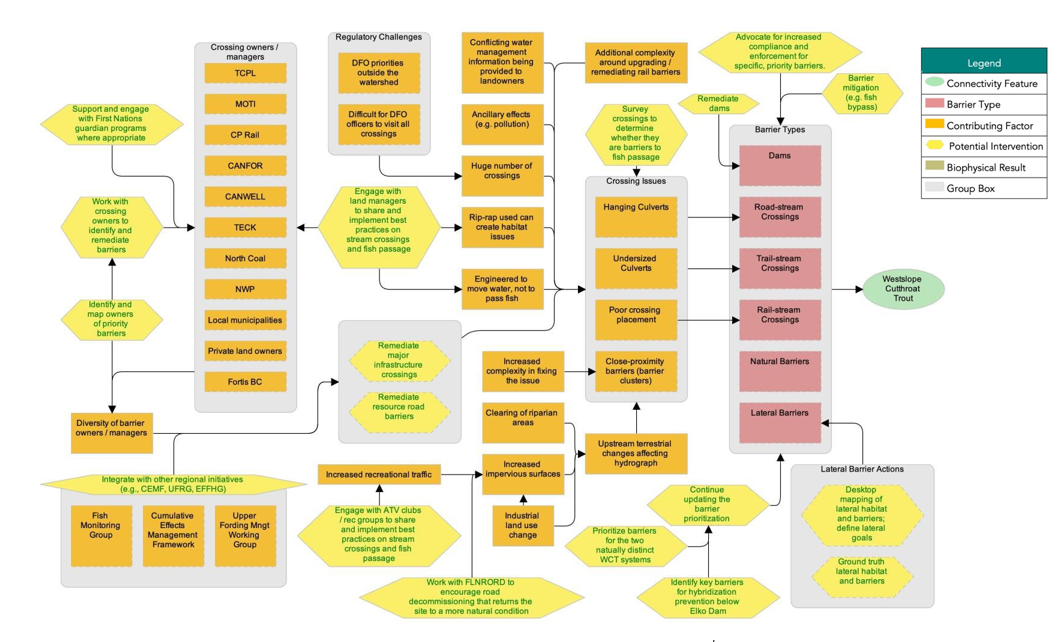
\includegraphics{content/images/situation-analysis.png}

}

\caption{\label{fig-sitan}Situation analysis developed by the planning
team to identify factors that contribute to fragmentation (orange boxes)
and potential strategies/actions to improve connectivity (yellow
hexagons) for Westslope Cutthroat Trout in the Elk River watershed.}

\end{figure}%

\section*{Strategies \& Actions}\label{strategies-actions}
\addcontentsline{toc}{section}{Strategies \& Actions}

\markright{Strategies \& Actions}

Effectiveness evaluation of identified conservation strategies and
associated actions to improve connectivity for Westslope Cutthroat Trout
in the Elk River watershed. The planning team identified two broad
strategies to implement through this WCRP, 1) barrier remediation and 2)
barrier prevention. Individual actions were qualitatively evaluated
based on the anticipated effect each action will have on realizing
on-the-ground gains in connectivity. Effectiveness ratings are based on
a combination of ``Feasibility'' and ``Impact'', Feasibility is defined
as the degree to which the project team can implement the action within
realistic constraints (financial, time, ethical, etc.) and Impact is the
degree to which the action is likely to contribute to achieving one or
more of the goals established in this plan.

\section*{Strategy 1: Barrier
Remediation}\label{strategy-1-barrier-remediation}
\addcontentsline{toc}{section}{Strategy 1: Barrier Remediation}

\markright{Strategy 1: Barrier Remediation}

\begin{longtable}[]{@{}llllll@{}}

\caption{\label{tbl-S1}Strategy 1}

\tabularnewline

\caption{}\label{T_c6bb7}\tabularnewline
\toprule\noalign{}
ID & Actions & Details & Feasibility & Impact & Effectiveness \\
\midrule\noalign{}
\endfirsthead
\toprule\noalign{}
ID & Actions & Details & Feasibility & Impact & Effectiveness \\
\midrule\noalign{}
\endhead
\bottomrule\noalign{}
\endlastfoot
1.1 & Remediate resource road barriers & This action represents some
projects that would be led by the planning team with conservation funds
(e.g., orphaned barriers or those owned by individuals), while other
remediation projects would be the responsibility of the barrier owner.
Industry will have to be engaged to successfully implement this
intervention. & High & Very high & Effective \\
1.2 & Remediate dams & Identify owners of dams that appear on the
intermediate barrier lists (see Appendix C) and engage with them to
explore technical and financial options. & Medium & Very high & Need
more information \\
1.3 & Remediate major infrastructure crossings & In most cases, the
planning team will engage with barrier owners, but the owners of the
barrier would be responsible for the financial cost of remediation. This
includes building relationships with CP rail to open a two-way
discussion on the scale, priority, and impact to their crossings on the
watershed. Include the financial and ecological cost/benefits of
remediation options in communication with infrastructure owners. &
Medium & Very high & Need more information \\
1.4 & Barrier mititgation & Examples may include installing fish ladders
on barriers that cannot be remediated; however, temporary mitigation
does not replace the need for barrier remediation and removal. There are
specific cases where temporary fixes are appropriate, but we will focus
on long-term solutions wherever possible. & Medium & High & Need more
information \\
1.5 & Work with crossing owners to identify and remediate barriers & &
High & High & Effective \\
1.6 & Advocate for increased compliance and enforcement for specific,
priority barriers & Request provincial and/or federal agencies to
require that targeted, high-priority barriers be remediated. This should
be a last resort after working to engage barrier owners and
ground-truthing the situation. It will be important to identify
obstacles to applying compliance and enforcement measures in order to
provide the appropriate information on these opportunities. & Very high
& High & Effective \\
1.7 & Work with FLNRORD to encourage road decommissioning that returns
sites to a more natural condition & Encourage sharing and implementation
of best practices for fish-passage-"friendly" road decommissioning. &
Very high & Very high & Very effective \\
1.8 & Integrate with other regional initiatives & Engage and pursue
coordination and collaboration with existing initiatives, (e.g., Elk
Valley Cumulative Effects Management Framework, the Upper Fording River
Recovery Group, the Elk Valley Fish and Fish Habitat Committee, and
terrestrial connectivity working groups). & Very high & Very high & Very
effective \\
1.9 & Raise funds to remediate barriers (ownership dependent) & Where
appropriate, collaborate within the planning team to raise conservation
funds for remediation projects. See ``Funding Sources'' for more
information. & High & Very high & Effective \\
1.1 & Knowledge Gap: Assess barriers by applying the provincial fish
passage framework & The first three steps are, (1) barrier assessments,
(2) habitat confirmations, and (3) remediation designs. Barrier
assessment data should be captured in the PSCIS database, which is
available to all partners. & Very high & Very high & Very effective \\
1.11 & Knowledge Gap: Identify key barriers for hybridization prevention
below Elko Dam & Barrier remediation below the Elko dam presents the
potential increased risk of hybridization of genetically pure Westslope
Cutthroat Trout populations due to reconnection to the Koocanusa
Reservoir. As such, prior to any decision, a series of site assessments
will need to be performed to assess the risk of hybridization. This
action does not directly contribute to the goals, but implementation is
necessary for the success of other actions. This strategy should be
revisited with First Nations and government agents to determine whether
it should be kept as a knowledge gap or if a different approach (i.e.,
to look at it from a watershed functionality perspective with less
concern about hybridization risks) should be adopted. & & & Need more
information \\
1.12 & Knowledge Gap: Identify and map owners of priority barriers & &
High & High & Effective \\
1.13 & Knowledge Gap: Prioritize barriers for the Upper Fording and
Grave-Harmon populations & Due to the importance of these genetically
pure populations within the watershed, ensure that barriers within these
systems are evaluated if they do not rank highly in initial barrier
prioritization efforts. & Very high & Very high & Very effective \\
1.14 & Knowledge Gap: Continue updating the barrier prioritization model
& The model process will be finalized, and prioritizations will be
updated as new information becomes available. & Very high & Very high &
Very effective \\
1.15 & Knowledge Gap: Desktop mapping of lateral habitat and barriers;
define lateral connectivity goals & This action does not directly
contribute to the current goals, but setting lateral goals is a
priority. Lateral barriers are considered a low threat in the Elk
valley, however work on a provincial scale is underway to determine the
impact of rail lines on lateral habitats. & & & Need more information \\
1.16 & Knowledge gap: Ground truth lateral habitat and barriers & This
action does not directly contribute to the current goals, but is an
important step following action 1.15. & & & Need more information \\
1.17 & Knowledge gap: Monitor temperature and flows; assess
effectiveness of barrier remediation projects & Effectiveness monitoring
study design (Lotic) for remediation sites. \$35K monitoring equipment
for ERA (CNFASAR). & & & Need more information \\

\end{longtable}

\section*{Strategy 2: Barrier
Prevention}\label{strategy-2-barrier-prevention}
\addcontentsline{toc}{section}{Strategy 2: Barrier Prevention}

\markright{Strategy 2: Barrier Prevention}

\begin{longtable}[]{@{}llllll@{}}

\caption{\label{tbl-S2}Strategy 2}

\tabularnewline

\caption{}\label{T_131c4}\tabularnewline
\toprule\noalign{}
ID & Actions & Details & Feasibility & Impact & Effectiveness \\
\midrule\noalign{}
\endfirsthead
\toprule\noalign{}
ID & Actions & Details & Feasibility & Impact & Effectiveness \\
\midrule\noalign{}
\endhead
\bottomrule\noalign{}
\endlastfoot
2.1 & Engage with land managers to share and implement best practices on
stream crossings and fish passage & This should include encouraging
better consultation before crossings are installed in the first place. &
High & High & Effective \\
2.2 & Support and engage with First Nations guardians programs where
appropriate & This could include approaching KNC about their existing
guardian program. & Very high & High & Effective \\
2.3 & Engage with ATV clubs/recreation groups to share and implement
best practices on stream crossings and fish passage & Trail-stream
crossings have a low extent and severity in the watershed, and it is
unlikely that ATV groups are creating barriers to fish passage. & High &
Low & Not Effective \\

\end{longtable}

\section*{Theories of Change \&
Objectives}\label{theories-of-change-objectives}
\addcontentsline{toc}{section}{Theories of Change \& Objectives}

\markright{Theories of Change \& Objectives}

Theories of Change are explicit assumptions around how the identified
actions will achieve gains in connectivity and contribute towards
reaching the goals of the plan. To develop Theories of Change, the
planning team developed explicit assumptions for each strategy which
helped to clarify the rationale used for undertaking actions and
provided an opportunity for feedback on invalid assumptions or missing
opportunities. The Theories of Change are results oriented and clearly
define the expected outcome. The following theory of change models were
developed by the WCRP planning team to ``map'' the causal (``if-then'')
progression of assumptions of how the actions within a strategy work
together to achieve project goals.

\begin{figure}

\centering{

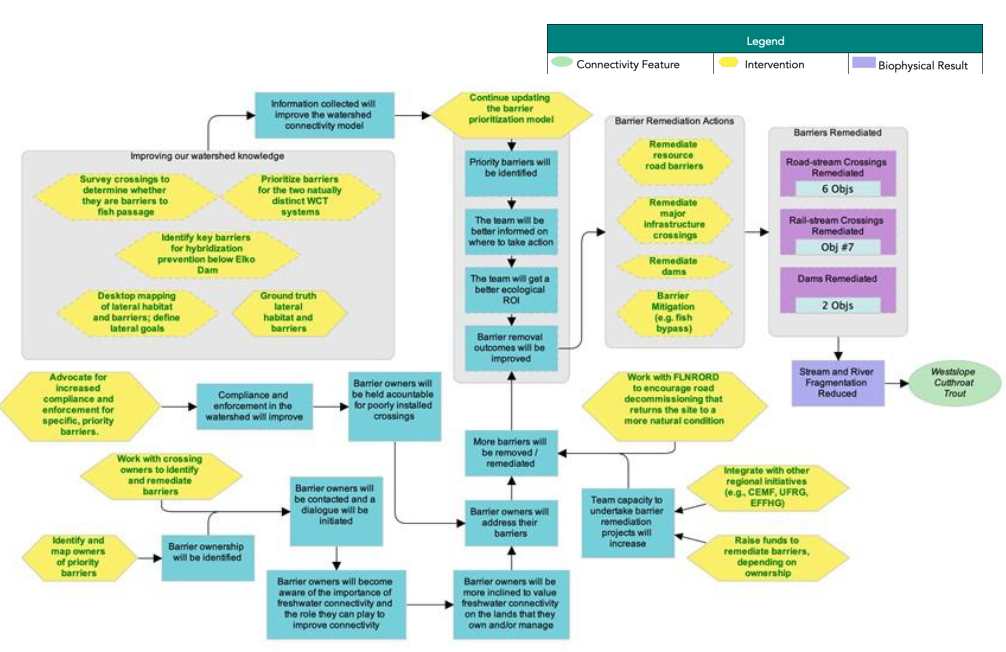
\includegraphics{content/images/flowchart-barrier-rem.png}

}

\caption{\label{fig-stra1}Theory of change developed by the planning
team for the actions identified under Strategy 1: Barrier Remediation in
the Elk River watershed.}

\end{figure}%

\begin{figure}

\centering{

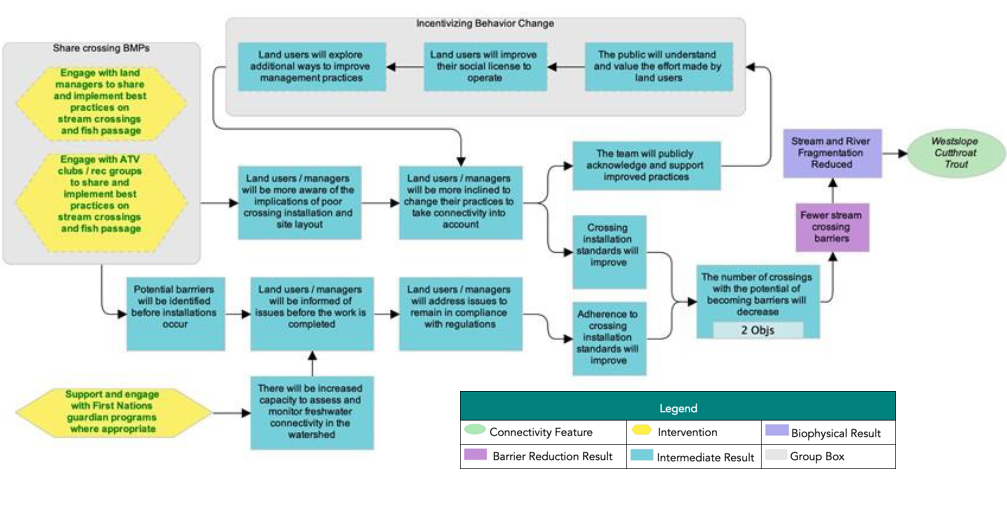
\includegraphics{content/images/flowchart-barrier-prevention.png}

}

\caption{\label{fig-stra2}Theory of change developed by the planning
team for the actions identified under Strategy 2: Barrier Prevention in
the Elk River watershed.}

\end{figure}%

\section*{Operational Plan}\label{operational-plan-1}
\addcontentsline{toc}{section}{Operational Plan}

\markright{Operational Plan}

The operational plan represents a preliminary exercise undertaken by the
planning team to identify the potential leads, potential participants,
and estimated cost for the implementation of each action in the Elk
River watershed. Table 8 summarizes individuals, groups, or
organizations that the planning team felt could lead or participate in
the implementation of the plan and should be interpreted as the first
step in on-going planning and engagement to develop more detailed plan
for entries into this table. The individuals, groups, and organizations
listed under the ``Lead(s)'' or ``Potential Participants'' columns are
those that provisionally expressed interest in participating in one of
those roles or were suggested by the planning team for further
engagement (denoted in parentheses), for those that are not members of
the planning team. The leads, participants, and estimated costs in the
operational plan are not binding nor an official commitment of
resources, but rather provide a roadmap for future coordination and
engagement to work towards implementation of the WCRP.

\begin{longtable}[]{@{}llll@{}}

\caption{\label{tbl-opplan}Operational plan to support the
implementation of strategies and actions to improve connectivity for
target species in the Horsefly River watershed.}

\tabularnewline

\caption{}\label{T_58d73}\tabularnewline
\toprule\noalign{}
Strategy / Actions & Lead(s) & Participants & Total Budget \\
\midrule\noalign{}
\endfirsthead
\toprule\noalign{}
Strategy / Actions & Lead(s) & Participants & Total Budget \\
\midrule\noalign{}
\endhead
\bottomrule\noalign{}
\endlastfoot
Strategy 1: Crossing Remediation & & & \$16,137,390.00 \\
1.1 - Remediate resource road barriers & CWF & & \$8,500,000.00 \\
1.2 - Remediate dams & CWF & & \$435,000,000.00 \\
1.3 - Remediate major infrastructure crossings & & CWF &
\$6,700,000.00 \\
1.4 - Barrier mititgation & CWF, SERN & CWF & *Built-in to 1.1 and
1.2 \\
1.5 - Work with crossing owners to identify and remediate barriers & Elk
River Alliance (ERA) & (Windsight), CWF & \$20,000 \\
1.6 - Advocate for increased compliance and enforcement for specific,
priority barriers & ERA & (Windsight), CWF & \$20,000.00 \\
1.7 - Work with FLNRORD to encourage road decommissioning that returns
sites to a more natural condition & ERA & (Windsight) & \$5,000.00 \\
1.8 - Integrate with other regional initiatives & CWF & ERA &
\$25,000.00 \\
1.9 - Raise funds to remediate barriers (ownership dependent) & CWF & &
\$200,000.00 \\
1.10 - Knowledge Gap: Assess barriers by applying the provincial fish
passage framework & CWF & & \$84,890.00 \\
1.11 - Knowledge Gap: Identify key barriers for hybridization prevention
below Elko Dam & & CWF & \$11,000.00 \\
1.12 - Knowledge Gap: Identify and map owners of priority barriers & ERA
& CWF & \$1,500.00 \\
1.13 - Knowledge Gap: Prioritize barriers for the Upper Fording and
Grave-Harmon populations & CWF & & Completed \\
1.14 - Knowledge Gap: Continue updating the barrier prioritization model
& CWF & & \$50,000 \\
1.15 - Knowledge Gap: Desktop mapping of lateral habitat and barriers;
define lateral connectivity goals & ERA & CWF & \$20,000.00 \\
1.16 - Knowledge gap: Ground truth lateral habitat and barriers & & CWF,
ERA & \$65,000 \\
1.17 - Knowledge gap: Monitor temperature and flows; assess
effectiveness of barrier remediation projects & ERA & CWF & \$50,000 \\
Strategy 2: Barrier Prevention & & & \$250,000.00 \\
2.1 - Engage with land managers to share and implement best practices on
stream crossings and fish passage & ERA & CWF & \$100,000.00 \\
2.2 - Support and engage with First Nations guardians programs where
appropriate & & CWF, KNC? & \$140,000.00 \\
2.3 - Engage with ATV clubs/recreation groups to share and implement
best practices on stream crossings and fish passage & & & \\
Total: & & & \$17,024,140.00 \\
Fundraising total: & & & \$9,024,140 \\
Proponent/government contribution total: & & & \$8,000,000 \\

\end{longtable}

\section*{Funding Sources}\label{funding-sources}
\addcontentsline{toc}{section}{Funding Sources}

\markright{Funding Sources}

\global\setlength{\Oldarrayrulewidth}{\arrayrulewidth}

\global\setlength{\Oldtabcolsep}{\tabcolsep}

\setlength{\tabcolsep}{2pt}

\renewcommand*{\arraystretch}{1.5}



\providecommand{\ascline}[3]{\noalign{\global\arrayrulewidth #1}\arrayrulecolor[HTML]{#2}\cline{#3}}

\begin{longtable}[c]{|p{3.58in}|p{11.20in}|p{1.01in}}

\caption{\label{tbl-fund1}Confirmed funding sources for plan
implementation in the Elk River watershed.}

\tabularnewline

\hhline{>{\arrayrulecolor[HTML]{666666}\global\arrayrulewidth=1.5pt}->{\arrayrulecolor[HTML]{666666}\global\arrayrulewidth=1.5pt}->{\arrayrulecolor[HTML]{666666}\global\arrayrulewidth=1.5pt}-}

\multicolumn{1}{>{\cellcolor[HTML]{008270}\raggedright}m{\dimexpr 3.58in+0\tabcolsep}}{\textcolor[HTML]{FFFFFF}{\fontsize{11}{11}\selectfont{\global\setmainfont{Arial}{Funding\ Source}}}} & \multicolumn{1}{>{\cellcolor[HTML]{008270}\raggedright}m{\dimexpr 11.2in+0\tabcolsep}}{\textcolor[HTML]{FFFFFF}{\fontsize{11}{11}\selectfont{\global\setmainfont{Arial}{Scope\ of\ Work}}}} & \multicolumn{1}{>{\cellcolor[HTML]{008270}\raggedright}m{\dimexpr 1.01in+0\tabcolsep}}{\textcolor[HTML]{FFFFFF}{\fontsize{11}{11}\selectfont{\global\setmainfont{Arial}{Amount}}}} \\

\noalign{\global\arrayrulewidth 0pt}\arrayrulecolor[HTML]{000000}

\hhline{>{\arrayrulecolor[HTML]{666666}\global\arrayrulewidth=1.5pt}->{\arrayrulecolor[HTML]{666666}\global\arrayrulewidth=1.5pt}->{\arrayrulecolor[HTML]{666666}\global\arrayrulewidth=1.5pt}-}\endfirsthead 

\hhline{>{\arrayrulecolor[HTML]{666666}\global\arrayrulewidth=1.5pt}->{\arrayrulecolor[HTML]{666666}\global\arrayrulewidth=1.5pt}->{\arrayrulecolor[HTML]{666666}\global\arrayrulewidth=1.5pt}-}

\multicolumn{1}{>{\cellcolor[HTML]{008270}\raggedright}m{\dimexpr 3.58in+0\tabcolsep}}{\textcolor[HTML]{FFFFFF}{\fontsize{11}{11}\selectfont{\global\setmainfont{Arial}{Funding\ Source}}}} & \multicolumn{1}{>{\cellcolor[HTML]{008270}\raggedright}m{\dimexpr 11.2in+0\tabcolsep}}{\textcolor[HTML]{FFFFFF}{\fontsize{11}{11}\selectfont{\global\setmainfont{Arial}{Scope\ of\ Work}}}} & \multicolumn{1}{>{\cellcolor[HTML]{008270}\raggedright}m{\dimexpr 1.01in+0\tabcolsep}}{\textcolor[HTML]{FFFFFF}{\fontsize{11}{11}\selectfont{\global\setmainfont{Arial}{Amount}}}} \\

\noalign{\global\arrayrulewidth 0pt}\arrayrulecolor[HTML]{000000}

\hhline{>{\arrayrulecolor[HTML]{666666}\global\arrayrulewidth=1.5pt}->{\arrayrulecolor[HTML]{666666}\global\arrayrulewidth=1.5pt}->{\arrayrulecolor[HTML]{666666}\global\arrayrulewidth=1.5pt}-}\endhead



\multicolumn{1}{>{\raggedright}m{\dimexpr 3.58in+0\tabcolsep}}{\textcolor[HTML]{000000}{\fontsize{11}{11}\selectfont{\global\setmainfont{Arial}{Fish\ and\ Wildlife\ Compensation\ Program}}}} & \multicolumn{1}{>{\raggedright}m{\dimexpr 11.2in+0\tabcolsep}}{\textcolor[HTML]{000000}{\fontsize{11}{11}\selectfont{\global\setmainfont{Arial}{Barrier\ assessments\ and\ habitat\ confirmations\ (2021-2022)}}}} & \multicolumn{1}{>{\raggedright}m{\dimexpr 1.01in+0\tabcolsep}}{\textcolor[HTML]{000000}{\fontsize{11}{11}\selectfont{\global\setmainfont{Arial}{\$63,000}}}} \\

\noalign{\global\arrayrulewidth 0pt}\arrayrulecolor[HTML]{000000}





\multicolumn{1}{>{\raggedright}m{\dimexpr 3.58in+0\tabcolsep}}{\textcolor[HTML]{000000}{\fontsize{11}{11}\selectfont{\global\setmainfont{Arial}{Environmental\ Damages\ Fund}}}} & \multicolumn{1}{>{\raggedright}m{\dimexpr 11.2in+0\tabcolsep}}{\textcolor[HTML]{000000}{\fontsize{11}{11}\selectfont{\global\setmainfont{Arial}{Engineering\ designs\ and\ remediation\ implementation\ (2021-2022,\ 2022-2023,\ 2023-2024)}}}} & \multicolumn{1}{>{\raggedright}m{\dimexpr 1.01in+0\tabcolsep}}{\textcolor[HTML]{000000}{\fontsize{11}{11}\selectfont{\global\setmainfont{Arial}{\$500,000}}}} \\

\noalign{\global\arrayrulewidth 0pt}\arrayrulecolor[HTML]{000000}





\multicolumn{1}{>{\raggedright}m{\dimexpr 3.58in+0\tabcolsep}}{\textcolor[HTML]{000000}{\fontsize{11}{11}\selectfont{\global\setmainfont{Arial}{Canada\ Nature\ Fund\ for\ Aquatic\ Species\ at\ Risk}}}} & \multicolumn{1}{>{\raggedright}m{\dimexpr 11.2in+0\tabcolsep}}{\textcolor[HTML]{000000}{\fontsize{11}{11}\selectfont{\global\setmainfont{Arial}{Conservation\ planning,\ barrier\ assessments,\ habitat\ confirmations,\ engineering\ designs,\ and\ barrier\ remediation\ (2019-2020,\ 2020-2021,\ 2021-2022,\ 2022-2023)}}}} & \multicolumn{1}{>{\raggedright}m{\dimexpr 1.01in+0\tabcolsep}}{\textcolor[HTML]{000000}{\fontsize{11}{11}\selectfont{\global\setmainfont{Arial}{\textasciitilde \$300,000}}}} \\

\noalign{\global\arrayrulewidth 0pt}\arrayrulecolor[HTML]{000000}





\multicolumn{1}{>{\raggedright}m{\dimexpr 3.58in+0\tabcolsep}}{\textcolor[HTML]{000000}{\fontsize{11}{11}\selectfont{\global\setmainfont{Arial}{}}}} & \multicolumn{1}{>{\raggedright}m{\dimexpr 11.2in+0\tabcolsep}}{\textcolor[HTML]{000000}{\fontsize{11}{11}\selectfont{\global\setmainfont{Arial}{}}}} & \multicolumn{1}{>{\raggedright}m{\dimexpr 1.01in+0\tabcolsep}}{\textcolor[HTML]{000000}{\fontsize{11}{11}\selectfont{\global\setmainfont{Arial}{}}}} \\

\noalign{\global\arrayrulewidth 0pt}\arrayrulecolor[HTML]{000000}

\hhline{>{\arrayrulecolor[HTML]{666666}\global\arrayrulewidth=1.5pt}->{\arrayrulecolor[HTML]{666666}\global\arrayrulewidth=1.5pt}->{\arrayrulecolor[HTML]{666666}\global\arrayrulewidth=1.5pt}-}


\end{longtable}

\arrayrulecolor[HTML]{000000}

\global\setlength{\arrayrulewidth}{\Oldarrayrulewidth}

\global\setlength{\tabcolsep}{\Oldtabcolsep}

\renewcommand*{\arraystretch}{1}

\global\setlength{\Oldarrayrulewidth}{\arrayrulewidth}

\global\setlength{\Oldtabcolsep}{\tabcolsep}

\setlength{\tabcolsep}{2pt}

\renewcommand*{\arraystretch}{1.5}



\providecommand{\ascline}[3]{\noalign{\global\arrayrulewidth #1}\arrayrulecolor[HTML]{#2}\cline{#3}}

\begin{longtable}[c]{|p{5.52in}|p{60.28in}}

\caption{\label{tbl-fund2}Potential funding sources for plan
implementation in the Elk River watershed. The Canadian Wildlife
Federation and the planning team can coordinate proposal submission
through these sources.}

\tabularnewline

\hhline{>{\arrayrulecolor[HTML]{666666}\global\arrayrulewidth=1.5pt}->{\arrayrulecolor[HTML]{666666}\global\arrayrulewidth=1.5pt}-}

\multicolumn{1}{>{\cellcolor[HTML]{008270}\raggedright}m{\dimexpr 5.52in+0\tabcolsep}}{\textcolor[HTML]{FFFFFF}{\fontsize{11}{11}\selectfont{\global\setmainfont{Arial}{Funding\ Source}}}} & \multicolumn{1}{>{\cellcolor[HTML]{008270}\raggedright}m{\dimexpr 60.28in+0\tabcolsep}}{\textcolor[HTML]{FFFFFF}{\fontsize{11}{11}\selectfont{\global\setmainfont{Arial}{Spending\ Restrictions\ and\ Other\ Consideration}}}} \\

\noalign{\global\arrayrulewidth 0pt}\arrayrulecolor[HTML]{000000}

\hhline{>{\arrayrulecolor[HTML]{666666}\global\arrayrulewidth=1.5pt}->{\arrayrulecolor[HTML]{666666}\global\arrayrulewidth=1.5pt}-}\endfirsthead 

\hhline{>{\arrayrulecolor[HTML]{666666}\global\arrayrulewidth=1.5pt}->{\arrayrulecolor[HTML]{666666}\global\arrayrulewidth=1.5pt}-}

\multicolumn{1}{>{\cellcolor[HTML]{008270}\raggedright}m{\dimexpr 5.52in+0\tabcolsep}}{\textcolor[HTML]{FFFFFF}{\fontsize{11}{11}\selectfont{\global\setmainfont{Arial}{Funding\ Source}}}} & \multicolumn{1}{>{\cellcolor[HTML]{008270}\raggedright}m{\dimexpr 60.28in+0\tabcolsep}}{\textcolor[HTML]{FFFFFF}{\fontsize{11}{11}\selectfont{\global\setmainfont{Arial}{Spending\ Restrictions\ and\ Other\ Consideration}}}} \\

\noalign{\global\arrayrulewidth 0pt}\arrayrulecolor[HTML]{000000}

\hhline{>{\arrayrulecolor[HTML]{666666}\global\arrayrulewidth=1.5pt}->{\arrayrulecolor[HTML]{666666}\global\arrayrulewidth=1.5pt}-}\endhead



\multicolumn{1}{>{\raggedright}m{\dimexpr 5.52in+0\tabcolsep}}{\textcolor[HTML]{000000}{\fontsize{11}{11}\selectfont{\global\setmainfont{Arial}{Land\ Based\ Investment\ Strategy}}}} & \multicolumn{1}{>{\raggedright}m{\dimexpr 60.28in+0\tabcolsep}}{\textcolor[HTML]{000000}{\fontsize{11}{11}\selectfont{\global\setmainfont{Arial}{Assessment\ and\ remediation\ of\ fish\ passage\ using\ provincial\ strategic\ approach.\ Primarily\ for\ remediation\ of\ Ministry-owned/orphaned\ barriers\ on\ forest\ service\ roads.}}}} \\

\noalign{\global\arrayrulewidth 0pt}\arrayrulecolor[HTML]{000000}





\multicolumn{1}{>{\raggedright}m{\dimexpr 5.52in+0\tabcolsep}}{\textcolor[HTML]{000000}{\fontsize{11}{11}\selectfont{\global\setmainfont{Arial}{Environmental\ Enhancement\ Fund}}}} & \multicolumn{1}{>{\raggedright}m{\dimexpr 60.28in+0\tabcolsep}}{\textcolor[HTML]{000000}{\fontsize{11}{11}\selectfont{\global\setmainfont{Arial}{Fish\ and\ wildlife\ passage\ improvements\ and\ restoration\ at\ stream\ and\ animal\ crossings\ at\ MOTI\ roads\ including\ culvert\ retrofits\ and\ replacement\ to\ restore\ Pacific\ salmon\ and\ trout\ access,\ and\ wildlife\ tunnels.\ Primarily\ for\ crossings\ linked\ to\ highway\ infrastructure.}}}} \\

\noalign{\global\arrayrulewidth 0pt}\arrayrulecolor[HTML]{000000}





\multicolumn{1}{>{\raggedright}m{\dimexpr 5.52in+0\tabcolsep}}{\textcolor[HTML]{000000}{\fontsize{11}{11}\selectfont{\global\setmainfont{Arial}{Habitat\ Conservation\ Trust\ Foundation\ Enhancement\ and\ Restoration\ Grants}}}} & \multicolumn{1}{>{\raggedright}m{\dimexpr 60.28in+0\tabcolsep}}{\textcolor[HTML]{000000}{\fontsize{11}{11}\selectfont{\global\setmainfont{Arial}{Projects\ that\ focus\ on\ freshwater\ wild\ fish,\ native\ wildlife\ species\ and\ their\ habitats,\ have\ the\ potential\ to\ achieve\ a\ significant\ conservation\ outcome,\ while\ maintaining\ or\ enhancing\ opportunities\ for\ fishing,\ hunting,\ trapping,\ wildlife\ viewing\ and\ associated\ outdoor\ recreational\ activities.\ Primary\ focus\ is\ on\ provincially\ managed\ fisheries\ such\ as\ Steelhead\ and\ Westslope\ Cutthroat\ Trout.\ Requires\ 50\%\ funding\ match.}}}} \\

\noalign{\global\arrayrulewidth 0pt}\arrayrulecolor[HTML]{000000}





\multicolumn{1}{>{\raggedright}m{\dimexpr 5.52in+0\tabcolsep}}{\textcolor[HTML]{000000}{\fontsize{11}{11}\selectfont{\global\setmainfont{Arial}{Environmental\ Damages\ Fund}}}} & \multicolumn{1}{>{\raggedright}m{\dimexpr 60.28in+0\tabcolsep}}{\textcolor[HTML]{000000}{\fontsize{11}{11}\selectfont{\global\setmainfont{Arial}{Direct\ funds\ received\ from\ fines,\ court\ orders\ and\ voluntary\ payments\ to\ priority\ projects\ that\ will\ benefit\ Canada’s\ natural\ environment,\ under\ 4\ categories\ of\ improvement\ (in\ order\ of\ preference):\ (1)\ restoration,\ (2)\ environmental\ quality\ improvement,\ (3)\ research\ and\ development,\ and\ (4)\ education\ and\ awareness.}}}} \\

\noalign{\global\arrayrulewidth 0pt}\arrayrulecolor[HTML]{000000}





\multicolumn{1}{>{\raggedright}m{\dimexpr 5.52in+0\tabcolsep}}{\textcolor[HTML]{000000}{\fontsize{11}{11}\selectfont{\global\setmainfont{Arial}{Fish\ and\ Wildlife\ Compensation\ Program}}}} & \multicolumn{1}{>{\raggedright}m{\dimexpr 60.28in+0\tabcolsep}}{\textcolor[HTML]{000000}{\fontsize{11}{11}\selectfont{\global\setmainfont{Arial}{Funding\ to\ conserve\ and\ enhance\ fish\ and\ wildlife\ in\ watersheds\ impacted\ by\ BC\ Hydro\ dams.\ Funding\ is\ for\ priority\ actions\ identified\ in\ the\ Columbia\ Region\ Action\ Plan.\ Funding\ available\ to\ First\ Nations,\ consultants,\ NGOs,\ individuals,\ agencies,\ and\ academic\ institutions.}}}} \\

\noalign{\global\arrayrulewidth 0pt}\arrayrulecolor[HTML]{000000}





\multicolumn{1}{>{\raggedright}m{\dimexpr 5.52in+0\tabcolsep}}{\textcolor[HTML]{000000}{\fontsize{11}{11}\selectfont{\global\setmainfont{Arial}{Habitat\ Stewardship\ Program\ for\ Aquatic\ Species\ at\ Risk}}}} & \multicolumn{1}{>{\raggedright}m{\dimexpr 60.28in+0\tabcolsep}}{\textcolor[HTML]{000000}{\fontsize{11}{11}\selectfont{\global\setmainfont{Arial}{Program\ for\ non-profits,\ Indigenous\ governments,\ academic\ institutions\ for\ activities\ that\ align\ with\ recovery\ actions\ identified\ in\ SARA\ recovery\ documents\ and/or\ COSEWIC\ assessment\ documents.\ Project\ must\ address\ one\ or\ more\ of\ 3\ broad\ categories:\ (1)\ Important\ habitat\ for\ aquatic\ species\ at\ risk\ is\ improved\ and/or\ managed\ to\ meet\ their\ recovery\ needs;\ (2)\ Threats\ to\ aquatic\ species\ at\ risk\ and/or\ their\ habitat\ are\ stopped,\ removed,\ and/or\ mitigated;\ (3)\ Collaboration\ and\ partnerships\ support\ the\ conservation\ and\ recovery\ of\ aquatic\ species\ at\ risk.\ Limited\ to\ at-risk\ species\ listed\ under\ COSEWIC\ and/or\ SARA\ as\ threatened,\ endangered\ or\ special\ concern.\ }}}} \\

\noalign{\global\arrayrulewidth 0pt}\arrayrulecolor[HTML]{000000}





\multicolumn{1}{>{\raggedright}m{\dimexpr 5.52in+0\tabcolsep}}{\textcolor[HTML]{000000}{\fontsize{11}{11}\selectfont{\global\setmainfont{Arial}{Canada\ Nature\ Fund\ for\ Aquatic\ Species\ at\ Risk}}}} & \multicolumn{1}{>{\raggedright}m{\dimexpr 60.28in+0\tabcolsep}}{\textcolor[HTML]{000000}{\fontsize{11}{11}\selectfont{\global\setmainfont{Arial}{Funding\ program\ aimed\ at\ addressing\ priority\ threats\ for\ aquatic\ species\ at\ risk\ listed\ as\ endangered,\ threatened\ or\ Special\ Concern\ by\ COSEWIC,\ as\ they\ align\ with\ existing\ federal,\ provincial\ or\ other\ local\ recovery\ plans.\ Limited\ to\ species\ in\ the\ Columbia\ and\ Fraser\ basins\ in\ BC,\ among\ other\ priority\ areas\ across\ Canada.\ Focus\ on\ multi-year,\ multi-partner\ initiatives\ that\ apply\ an\ ecosystem\ or\ multi-species\ approach\ and\ create\ a\ legacy\ by\ enabling\ recovery\ actions\ that\ carry\ beyond\ the\ life\ of\ the\ funding\ program.\ Amounts\ from\ \$100K-\$1M\ available\ per\ year.}}}} \\

\noalign{\global\arrayrulewidth 0pt}\arrayrulecolor[HTML]{000000}





\multicolumn{1}{>{\raggedright}m{\dimexpr 5.52in+0\tabcolsep}}{\textcolor[HTML]{000000}{\fontsize{11}{11}\selectfont{\global\setmainfont{Arial}{Aboriginal\ Fund\ for\ Species\ at\ Risk}}}} & \multicolumn{1}{>{\raggedright}m{\dimexpr 60.28in+0\tabcolsep}}{\textcolor[HTML]{000000}{\fontsize{11}{11}\selectfont{\global\setmainfont{Arial}{Program\ for\ Indigenous\ groups\ for\ activities\ that\ align\ with\ recovery\ actions\ identified\ in\ SARA\ recovery\ documents\ and/or\ COSEWIC\ assessment\ documents\ for\ species\ listed\ as\ Endangered,\ Threatened,\ or\ Special\ Concern\ by\ SARA\ or\ COSEWIC.\ Project\ must\ address\ one\ or\ more\ of\ 4\ broad\ categories:\ (1)\ Habitat\ for\ species\ at\ risk\ is\ improved\ and/or\ managed\ to\ meet\ their\ recovery\ needs;\ (2)\ Threats\ to\ species\ at\ risk\ and/or\ their\ habitat\ are\ stopped,\ removed\ and/or\ mitigated;\ (3)\ Collaboration,\ information\ sharing\ and\ partnership\ between\ Indigenous\ communities,\ governments\ and\ organizations\ and\ other\ interested\ parties\ (e.g.\ federal/provincial/territorial\ governments,\ academia,\ industry,\ private\ sector)\ is\ enhanced;\ and\ (4)\ Capacity\ within\ Indigenous\ communities,\ to\ lead\ in\ the\ stewardship\ of\ species\ at\ risk\ and\ contribute\ to\ broader\ SARA\ implementation,\ is\ strengthened.\ }}}} \\

\noalign{\global\arrayrulewidth 0pt}\arrayrulecolor[HTML]{000000}





\multicolumn{1}{>{\raggedright}m{\dimexpr 5.52in+0\tabcolsep}}{\textcolor[HTML]{000000}{\fontsize{11}{11}\selectfont{\global\setmainfont{Arial}{Colombia\ Basin\ Trust\ Envrionment\ Grants}}}} & \multicolumn{1}{>{\raggedright}m{\dimexpr 60.28in+0\tabcolsep}}{\textcolor[HTML]{000000}{\fontsize{11}{11}\selectfont{\global\setmainfont{Arial}{Small\ (<\$5K)\ and\ large\ grants\ (>\$5K)\ for\ First\ Nation\ communities,\ municipalities\ and\ regional\ districts.\ Businesses\ may\ be\ considered\ depending\ on\ the\ project\ and\ its\ broad\ community\ impact.\ Enhance\ or\ conserve\ ecosystems\ and/or\ species\ of\ conservation\ concern.\ Funding\ for\ water\ projects,\ environmental\ education\ projects,\ and\ ecosystems\ projects:\ 1)\ reduce\ the\ threat\ of\ significant\ invasive\ species\ to\ terrestrial\ and\ aquatic\ ecosystems;\ and\ 2)\ ecosystem\ related\ research\ projects\ that\ contribute\ to\ ecosystem\ conservation\ and/or\ enhancement.}}}} \\

\noalign{\global\arrayrulewidth 0pt}\arrayrulecolor[HTML]{000000}





\multicolumn{1}{>{\raggedright}m{\dimexpr 5.52in+0\tabcolsep}}{\textcolor[HTML]{000000}{\fontsize{11}{11}\selectfont{\global\setmainfont{Arial}{Federal\ Gas\ Tax\ Fund\ -\ Community\ Works\ Fund}}}} & \multicolumn{1}{>{\raggedright}m{\dimexpr 60.28in+0\tabcolsep}}{\textcolor[HTML]{000000}{\fontsize{11}{11}\selectfont{\global\setmainfont{Arial}{Funding\ available\ to\ local\ governments\ from\ federal\ gas\ tax,\ with\ funds\ to\ be\ allocated\ for\ a\ variety\ of\ municipal\ projects/initiatives,\ including\ local\ roads/bridges\ and\ disaster\ mitigation.}}}} \\

\noalign{\global\arrayrulewidth 0pt}\arrayrulecolor[HTML]{000000}





\multicolumn{1}{>{\raggedright}m{\dimexpr 5.52in+0\tabcolsep}}{\textcolor[HTML]{000000}{\fontsize{11}{11}\selectfont{\global\setmainfont{Arial}{Disaster\ Mitigation\ and\ Adaptation\ Fund}}}} & \multicolumn{1}{>{\raggedright}m{\dimexpr 60.28in+0\tabcolsep}}{\textcolor[HTML]{000000}{\fontsize{11}{11}\selectfont{\global\setmainfont{Arial}{For\ those\ projects\ where\ flood\ risk\ is\ high:\ Funding\ available\ to\ local,\ regional\ and\ provincial\ governments,\ private\ sector,\ non-profit\ organizations,\ and\ Indigenous\ groups\ for\ projects\ aimed\ at\ reducing\ the\ socio-economic,\ environmental\ and\ cultural\ impacts\ triggered\ by\ natural\ hazards\ and\ extreme\ weather\ events\ and\ taking\ into\ consideration\ current\ and\ future\ impacts\ of\ climate\ change\ in\ communities\ and\ infrastructure\ at\ high\ risk.\ Includes\ both\ new\ construction\ of\ public\ infrastructure\ and\ modification/reinforcement\ of\ existing\ infrastructure.\ Projects\ must\ have\ a\ minimum\ of\ \$20\ M\ in\ eligible\ expenditures\ and\ can\ be\ bundled\ together.}}}} \\

\noalign{\global\arrayrulewidth 0pt}\arrayrulecolor[HTML]{000000}





\multicolumn{1}{>{\raggedright}m{\dimexpr 5.52in+0\tabcolsep}}{\textcolor[HTML]{000000}{\fontsize{11}{11}\selectfont{\global\setmainfont{Arial}{Community\ Gaming\ Grants}}}} & \multicolumn{1}{>{\raggedright}m{\dimexpr 60.28in+0\tabcolsep}}{\textcolor[HTML]{000000}{\fontsize{11}{11}\selectfont{\global\setmainfont{Arial}{Funding\ for\ non-profit\ organizations\ (check\ funding\ program\ guidelines\ for\ specific\ eligibility\ requirements)\ for\ programs\ that\ help\ to\ protect\ and\ improve\ the\ environment\ by:\ (1)\ Conserving\ or\ revitalizing\ local\ ecosystems,\ (2)\ Reducing\ greenhouse\ gas\ emissions,\ (3)\ Providing\ community\ education\ or\ engagement\ opportunities\ related\ to\ the\ environment\ and\ agriculture\ or\ (4)\ Supporting\ the\ welfare\ of\ domestic\ animals\ and/or\ wildlife.\ Grants\ range\ from\ \$100K-250K\ per\ year.}}}} \\

\noalign{\global\arrayrulewidth 0pt}\arrayrulecolor[HTML]{000000}





\multicolumn{1}{>{\raggedright}m{\dimexpr 5.52in+0\tabcolsep}}{\textcolor[HTML]{000000}{\fontsize{11}{11}\selectfont{\global\setmainfont{Arial}{Sitka\ Foundation}}}} & \multicolumn{1}{>{\raggedright}m{\dimexpr 60.28in+0\tabcolsep}}{\textcolor[HTML]{000000}{\fontsize{11}{11}\selectfont{\global\setmainfont{Arial}{Funding\ for\ registered\ charities,\ universities,\ and\ government\ agencies\ (qualified\ Canadian\ organizations)\ for\ projects\ related\ to\ coastline\ and\ watershed\ conservation\ and\ climate\ change\ in\ 4\ key\ areas:\ (1)\ land,\ water,\ and\ ocean\ conservation,\ (2)\ scientific\ research\ for\ nature\ and\ the\ environment,\ (3)\ \ public\ engagement\ around\ the\ importance\ of\ a\ healthy\ environment,\ (4)\ innovative\ conservation\ efforts\ in\ Canadian\ communities,\ at\ the\ local,\ provincial,\ and\ federal\ levels}}}} \\

\noalign{\global\arrayrulewidth 0pt}\arrayrulecolor[HTML]{000000}





\multicolumn{1}{>{\raggedright}m{\dimexpr 5.52in+0\tabcolsep}}{\textcolor[HTML]{000000}{\fontsize{11}{11}\selectfont{\global\setmainfont{Arial}{TULA\ Foundation}}}} & \multicolumn{1}{>{\raggedright}m{\dimexpr 60.28in+0\tabcolsep}}{\textcolor[HTML]{000000}{\fontsize{11}{11}\selectfont{\global\setmainfont{Arial}{Supports\ various\ environmental\ programs\ of\ interest\ to\ the\ Foundation\ on\ a\ case-by-case\ basis.}}}} \\

\noalign{\global\arrayrulewidth 0pt}\arrayrulecolor[HTML]{000000}





\multicolumn{1}{>{\raggedright}m{\dimexpr 5.52in+0\tabcolsep}}{\textcolor[HTML]{000000}{\fontsize{11}{11}\selectfont{\global\setmainfont{Arial}{Vancouver\ Foundation}}}} & \multicolumn{1}{>{\raggedright}m{\dimexpr 60.28in+0\tabcolsep}}{\textcolor[HTML]{000000}{\fontsize{11}{11}\selectfont{\global\setmainfont{Arial}{Granting\ agency\ for\ community,\ social\ and\ environmental\ initiatives\ for\ qualified\ Canadian\ organizations\ (charitable\ organizations,\ universities,\ government\ agencies).\ Granting\ programs\ change\ on\ an\ annual\ basis.}}}} \\

\noalign{\global\arrayrulewidth 0pt}\arrayrulecolor[HTML]{000000}





\multicolumn{1}{>{\raggedright}m{\dimexpr 5.52in+0\tabcolsep}}{\textcolor[HTML]{000000}{\fontsize{11}{11}\selectfont{\global\setmainfont{Arial}{BC\ Conservation\ Foundation\ Small\ Project\ Fund}}}} & \multicolumn{1}{>{\raggedright}m{\dimexpr 60.28in+0\tabcolsep}}{\textcolor[HTML]{000000}{\fontsize{11}{11}\selectfont{\global\setmainfont{Arial}{Funding\ available\ to\ Non-profits,\ fish\ and\ wildlife\ clubs\ (sportsmen’s\ associations),\ businesses,\ local/regional\ governments,\ public\ organizations\ and\ First\ Nations\ for\ projects\ with\ demonstrated\ positive\ impact\ for\ fish,\ wildlife\ and\ habitat,\ including\ outreach\ programs.\ Preference\ given\ to\ projects\ where\ BCCF\ is\ not\ the\ sole\ funder.}}}} \\

\noalign{\global\arrayrulewidth 0pt}\arrayrulecolor[HTML]{000000}





\multicolumn{1}{>{\raggedright}m{\dimexpr 5.52in+0\tabcolsep}}{\textcolor[HTML]{000000}{\fontsize{11}{11}\selectfont{\global\setmainfont{Arial}{Real\ Estate\ Foundation\ of\ BC\ General\ Grants}}}} & \multicolumn{1}{>{\raggedright}m{\dimexpr 60.28in+0\tabcolsep}}{\textcolor[HTML]{000000}{\fontsize{11}{11}\selectfont{\global\setmainfont{Arial}{Funding\ for\ First\ Nations,\ charities\ and\ societies,\ non-governmental\ organizations,\ universities\ and\ colleges,\ trade\ associations,\ local\ and\ regional\ governments,\ and\ social\ enterprises\ registered\ as\ C3s\ for\ sustainable\ land\ use\ and\ real\ estate\ practices\ in\ BC.\ Funds\ up\ to\ 50\%\ of\ cash\ portion\ of\ a\ project.}}}} \\

\noalign{\global\arrayrulewidth 0pt}\arrayrulecolor[HTML]{000000}

\hhline{>{\arrayrulecolor[HTML]{666666}\global\arrayrulewidth=1.5pt}->{\arrayrulecolor[HTML]{666666}\global\arrayrulewidth=1.5pt}-}


\end{longtable}

\arrayrulecolor[HTML]{000000}

\global\setlength{\arrayrulewidth}{\Oldarrayrulewidth}

\global\setlength{\tabcolsep}{\Oldtabcolsep}

\renewcommand*{\arraystretch}{1}

\chapter*{Data Download and Methods}\label{data-download-and-methods}
\addcontentsline{toc}{chapter}{Data Download and Methods}

\markboth{Data Download and Methods}{Data Download and Methods}

\section*{Modelled Anadromous Salmon Habitat
Maps}\label{modelled-anadromous-salmon-habitat-maps}
\addcontentsline{toc}{section}{Modelled Anadromous Salmon Habitat Maps}

\markright{Modelled Anadromous Salmon Habitat Maps}

High-resolution PDF maps of the Elk River watershed and model results
can be accessed here. The watershed is divided into multiple map sheets
to allow for detailed examination of modelled habitat and priority
barriers identified through this planning process. The locations of WCRP
priority barriers and associated map sheet numbers are shown below. In
each individual map sheet, priority barriers are symbolized using the
following notation:
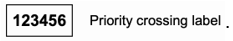
\includegraphics{content/images/priority-crossing-label.png}

\begin{figure}

\centering{

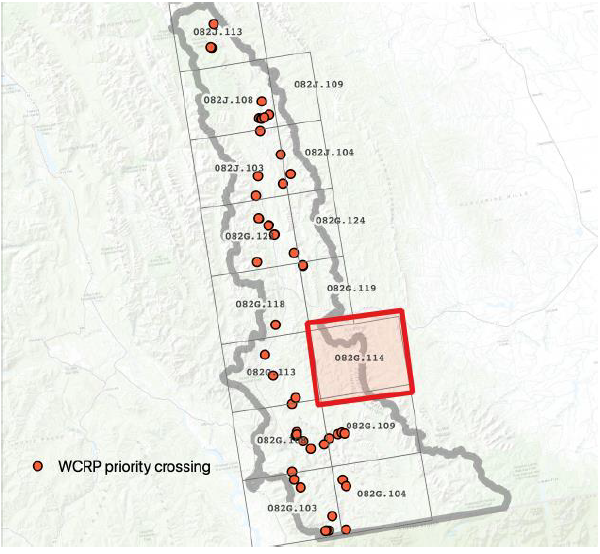
\includegraphics{content/images/overview-map-elkr.png}

}

\caption{\label{fig-over}Elk River watershed overview map identifying
the portions of the watershed covered by each map sheet (grey squares)
and the prioritized barriers on the intermediate barrier list (orange
points; see Appendix C).}

\end{figure}%

\section*{Connectivity Status Assessment
Methods}\label{connectivity-status-assessment-methods}
\addcontentsline{toc}{section}{Connectivity Status Assessment Methods}

\markright{Connectivity Status Assessment Methods}

The connectivity status assessment for Westslope Cutthroat Trout in the
Elk River watershed builds on existing connectivity modelling work
undertaken by the BC Fish Passage Technical Working Group, resulting in
a flexible, customizable open-source spatial model called
\href{https://github.com/smnorris/bcfishpass}{``bcfishpass''}. The model
spatially locates known and modelled barriers to fish passage,
identifies potential spawning and rearing habitat for Westslope
Cutthroat Trout, and estimates the amount of habitat that is currently
accessible as part of the Longest Fragment for each WCRP unit. The
Longest Fragment approach is adapted from Díaz and Habit (2021) and is
calculated as the ratio between the length of largest connected set of
habitat patches and the total length of all habitat patches in each WCRP
unit. In the Elk River watershed, the longest fragment represents the
mainstem Elk River and all currently connected tributaries, both
upstream and downstream of the Elko Dam. As such, meeting the
connectivity goals set in this plan requires prioritizing barriers for
remediation that will reconnect tributaries to the existing longest
fragments see \href{barrier-prioritization.qmd}{barrier prioritzation}.

The model uses an adapted version of the Intrinsic Potential (IP) fish
habitat modelling framework (see Sheer et al. (2009) for an overview of
the IP framework). The habitat model uses two geomorphic characteristics
of the stream network --- channel gradient and mean annual discharge ---
to identify potential spawning habitat and rearing habitat for target
species. For the purposes of this plan, rearing habitat is used as an
umbrella term to capture the requirements for Westslope Cutthroat Trout
rearing, maintenance, and overwintering habitat. The habitat model does
not attempt to definitively map each habitat type nor estimate habitat
quality, but rather identifies stream segments that have high potential
to support spawning or rearing habitat for Westslope Cutthroat Trout
based on the geomorphic characteristics of the segment. For more details
on the connectivity and habitat model structure and parameters, please
see Mazany-Wright, Norris, et al. (2021a). The variables and thresholds
used to model potential spawning and rearing habitat are summarized
below. The quantity of modelled habitat was aggregated for each habitat
type to inform the two KEAs --- Accessible Habitat Upstream of Elko Dam
and Accessible Habitat Downstream of Elko Dam --- and represents a
linear measure of potential habitat. To recognize the rearing value
provided by features represented by polygons (e.g., lakes for
overwintering) a multiplier of 1.5x the length of the stream segments
flowing through the polygons was applied.

\global\setlength{\Oldarrayrulewidth}{\arrayrulewidth}

\global\setlength{\Oldtabcolsep}{\tabcolsep}

\setlength{\tabcolsep}{2pt}

\renewcommand*{\arraystretch}{1.5}



\providecommand{\ascline}[3]{\noalign{\global\arrayrulewidth #1}\arrayrulecolor[HTML]{#2}\cline{#3}}

\begin{longtable}[c]{|p{3.00in}|p{3.59in}|p{2.83in}|p{3.47in}|p{3.04in}|p{2.43in}}

\caption{\label{tbl-param}Parameters and thresholds used to inform the
Intrinsic Potential habitat model for spawning and rearing habitat for
Westslope Cutthroat Trout in the Elk River watershed.}

\tabularnewline

\hhline{>{\arrayrulecolor[HTML]{666666}\global\arrayrulewidth=1.5pt}->{\arrayrulecolor[HTML]{666666}\global\arrayrulewidth=1.5pt}->{\arrayrulecolor[HTML]{666666}\global\arrayrulewidth=1.5pt}->{\arrayrulecolor[HTML]{666666}\global\arrayrulewidth=1.5pt}->{\arrayrulecolor[HTML]{666666}\global\arrayrulewidth=1.5pt}->{\arrayrulecolor[HTML]{666666}\global\arrayrulewidth=1.5pt}-}

\multicolumn{1}{>{\cellcolor[HTML]{008270}\raggedright}m{\dimexpr 3in+0\tabcolsep}}{\textcolor[HTML]{FFFFFF}{\fontsize{11}{11}\selectfont{\global\setmainfont{Arial}{Spawning\ Habitat\ Channel\ Gradient\ (\%)}}}} & \multicolumn{1}{>{\cellcolor[HTML]{008270}\raggedright}m{\dimexpr 3.59in+0\tabcolsep}}{\textcolor[HTML]{FFFFFF}{\fontsize{11}{11}\selectfont{\global\setmainfont{Arial}{Spawning\ Habitat\ Mean\ annual\ discharge\ (m3/s)}}}} & \multicolumn{1}{>{\cellcolor[HTML]{008270}\raggedright}m{\dimexpr 2.83in+0\tabcolsep}}{\textcolor[HTML]{FFFFFF}{\fontsize{11}{11}\selectfont{\global\setmainfont{Arial}{Rearing\ Habitat\ Channel\ gradient\ (\%)}}}} & \multicolumn{1}{>{\cellcolor[HTML]{008270}\raggedright}m{\dimexpr 3.47in+0\tabcolsep}}{\textcolor[HTML]{FFFFFF}{\fontsize{11}{11}\selectfont{\global\setmainfont{Arial}{Rearing\ Habitat\ Mean\ Annual\ discharge\ (m3/s)}}}} & \multicolumn{1}{>{\cellcolor[HTML]{008270}\raggedright}m{\dimexpr 3.04in+0\tabcolsep}}{\textcolor[HTML]{FFFFFF}{\fontsize{11}{11}\selectfont{\global\setmainfont{Arial}{Rearing\ Habitat\ Minimum\ Lake\ area\ (ha)}}}} & \multicolumn{1}{>{\cellcolor[HTML]{008270}\raggedright}m{\dimexpr 2.43in+0\tabcolsep}}{\textcolor[HTML]{FFFFFF}{\fontsize{11}{11}\selectfont{\global\setmainfont{Arial}{Rearing\ Habitat\ Multiplier\ (1.5x)}}}} \\

\noalign{\global\arrayrulewidth 0pt}\arrayrulecolor[HTML]{000000}

\hhline{>{\arrayrulecolor[HTML]{666666}\global\arrayrulewidth=1.5pt}->{\arrayrulecolor[HTML]{666666}\global\arrayrulewidth=1.5pt}->{\arrayrulecolor[HTML]{666666}\global\arrayrulewidth=1.5pt}->{\arrayrulecolor[HTML]{666666}\global\arrayrulewidth=1.5pt}->{\arrayrulecolor[HTML]{666666}\global\arrayrulewidth=1.5pt}->{\arrayrulecolor[HTML]{666666}\global\arrayrulewidth=1.5pt}-}\endfirsthead 

\hhline{>{\arrayrulecolor[HTML]{666666}\global\arrayrulewidth=1.5pt}->{\arrayrulecolor[HTML]{666666}\global\arrayrulewidth=1.5pt}->{\arrayrulecolor[HTML]{666666}\global\arrayrulewidth=1.5pt}->{\arrayrulecolor[HTML]{666666}\global\arrayrulewidth=1.5pt}->{\arrayrulecolor[HTML]{666666}\global\arrayrulewidth=1.5pt}->{\arrayrulecolor[HTML]{666666}\global\arrayrulewidth=1.5pt}-}

\multicolumn{1}{>{\cellcolor[HTML]{008270}\raggedright}m{\dimexpr 3in+0\tabcolsep}}{\textcolor[HTML]{FFFFFF}{\fontsize{11}{11}\selectfont{\global\setmainfont{Arial}{Spawning\ Habitat\ Channel\ Gradient\ (\%)}}}} & \multicolumn{1}{>{\cellcolor[HTML]{008270}\raggedright}m{\dimexpr 3.59in+0\tabcolsep}}{\textcolor[HTML]{FFFFFF}{\fontsize{11}{11}\selectfont{\global\setmainfont{Arial}{Spawning\ Habitat\ Mean\ annual\ discharge\ (m3/s)}}}} & \multicolumn{1}{>{\cellcolor[HTML]{008270}\raggedright}m{\dimexpr 2.83in+0\tabcolsep}}{\textcolor[HTML]{FFFFFF}{\fontsize{11}{11}\selectfont{\global\setmainfont{Arial}{Rearing\ Habitat\ Channel\ gradient\ (\%)}}}} & \multicolumn{1}{>{\cellcolor[HTML]{008270}\raggedright}m{\dimexpr 3.47in+0\tabcolsep}}{\textcolor[HTML]{FFFFFF}{\fontsize{11}{11}\selectfont{\global\setmainfont{Arial}{Rearing\ Habitat\ Mean\ Annual\ discharge\ (m3/s)}}}} & \multicolumn{1}{>{\cellcolor[HTML]{008270}\raggedright}m{\dimexpr 3.04in+0\tabcolsep}}{\textcolor[HTML]{FFFFFF}{\fontsize{11}{11}\selectfont{\global\setmainfont{Arial}{Rearing\ Habitat\ Minimum\ Lake\ area\ (ha)}}}} & \multicolumn{1}{>{\cellcolor[HTML]{008270}\raggedright}m{\dimexpr 2.43in+0\tabcolsep}}{\textcolor[HTML]{FFFFFF}{\fontsize{11}{11}\selectfont{\global\setmainfont{Arial}{Rearing\ Habitat\ Multiplier\ (1.5x)}}}} \\

\noalign{\global\arrayrulewidth 0pt}\arrayrulecolor[HTML]{000000}

\hhline{>{\arrayrulecolor[HTML]{666666}\global\arrayrulewidth=1.5pt}->{\arrayrulecolor[HTML]{666666}\global\arrayrulewidth=1.5pt}->{\arrayrulecolor[HTML]{666666}\global\arrayrulewidth=1.5pt}->{\arrayrulecolor[HTML]{666666}\global\arrayrulewidth=1.5pt}->{\arrayrulecolor[HTML]{666666}\global\arrayrulewidth=1.5pt}->{\arrayrulecolor[HTML]{666666}\global\arrayrulewidth=1.5pt}-}\endhead



\multicolumn{1}{>{\raggedright}m{\dimexpr 3in+0\tabcolsep}}{\textcolor[HTML]{000000}{\fontsize{11}{11}\selectfont{\global\setmainfont{Arial}{0-3\ [1]\ [2]}}}} & \multicolumn{1}{>{\raggedright}m{\dimexpr 3.59in+0\tabcolsep}}{\textcolor[HTML]{000000}{\fontsize{11}{11}\selectfont{\global\setmainfont{Arial}{0.46-322.5\ [3][4][5][6][7]}}}} & \multicolumn{1}{>{\raggedright}m{\dimexpr 2.83in+0\tabcolsep}}{\textcolor[HTML]{000000}{\fontsize{11}{11}\selectfont{\global\setmainfont{Arial}{0-5\ [5][8]}}}} & \multicolumn{1}{>{\raggedright}m{\dimexpr 3.47in+0\tabcolsep}}{\textcolor[HTML]{000000}{\fontsize{11}{11}\selectfont{\global\setmainfont{Arial}{0.28-100\ [9]}}}} & \multicolumn{1}{>{\raggedright}m{\dimexpr 3.04in+0\tabcolsep}}{\textcolor[HTML]{000000}{\fontsize{11}{11}\selectfont{\global\setmainfont{Arial}{}}}} & \multicolumn{1}{>{\raggedright}m{\dimexpr 2.43in+0\tabcolsep}}{\textcolor[HTML]{000000}{\fontsize{11}{11}\selectfont{\global\setmainfont{Arial}{}}}} \\

\noalign{\global\arrayrulewidth 0pt}\arrayrulecolor[HTML]{000000}





\multicolumn{1}{>{\raggedright}m{\dimexpr 3in+0\tabcolsep}}{\textcolor[HTML]{000000}{\fontsize{11}{11}\selectfont{\global\setmainfont{Arial}{0-5\ [6][10]}}}} & \multicolumn{1}{>{\raggedright}m{\dimexpr 3.59in+0\tabcolsep}}{\textcolor[HTML]{000000}{\fontsize{11}{11}\selectfont{\global\setmainfont{Arial}{0.164-59.15\ [3][4][5][10][11]}}}} & \multicolumn{1}{>{\raggedright}m{\dimexpr 2.83in+0\tabcolsep}}{\textcolor[HTML]{000000}{\fontsize{11}{11}\selectfont{\global\setmainfont{Arial}{0-5\ [8][12]}}}} & \multicolumn{1}{>{\raggedright}m{\dimexpr 3.47in+0\tabcolsep}}{\textcolor[HTML]{000000}{\fontsize{11}{11}\selectfont{\global\setmainfont{Arial}{0.03-40\ [8][13]}}}} & \multicolumn{1}{>{\raggedright}m{\dimexpr 3.04in+0\tabcolsep}}{\textcolor[HTML]{000000}{\fontsize{11}{11}\selectfont{\global\setmainfont{Arial}{}}}} & \multicolumn{1}{>{\raggedright}m{\dimexpr 2.43in+0\tabcolsep}}{\textcolor[HTML]{000000}{\fontsize{11}{11}\selectfont{\global\setmainfont{Arial}{Wetland}}}} \\

\noalign{\global\arrayrulewidth 0pt}\arrayrulecolor[HTML]{000000}





\multicolumn{1}{>{\raggedright}m{\dimexpr 3in+0\tabcolsep}}{\textcolor[HTML]{000000}{\fontsize{11}{11}\selectfont{\global\setmainfont{Arial}{0-2\ [14][15]}}}} & \multicolumn{1}{>{\raggedright}m{\dimexpr 3.59in+0\tabcolsep}}{\textcolor[HTML]{000000}{\fontsize{11}{11}\selectfont{\global\setmainfont{Arial}{0.175-65\ [3][4][5][6]}}}} & \multicolumn{1}{>{\raggedright}m{\dimexpr 2.83in+0\tabcolsep}}{\textcolor[HTML]{000000}{\fontsize{11}{11}\selectfont{\global\setmainfont{Arial}{}}}} & \multicolumn{1}{>{\raggedright}m{\dimexpr 3.47in+0\tabcolsep}}{\textcolor[HTML]{000000}{\fontsize{11}{11}\selectfont{\global\setmainfont{Arial}{}}}} & \multicolumn{1}{>{\raggedright}m{\dimexpr 3.04in+0\tabcolsep}}{\textcolor[HTML]{000000}{\fontsize{11}{11}\selectfont{\global\setmainfont{Arial}{200\ [5]}}}} & \multicolumn{1}{>{\raggedright}m{\dimexpr 2.43in+0\tabcolsep}}{\textcolor[HTML]{000000}{\fontsize{11}{11}\selectfont{\global\setmainfont{Arial}{Lake}}}} \\

\noalign{\global\arrayrulewidth 0pt}\arrayrulecolor[HTML]{000000}

\hhline{>{\arrayrulecolor[HTML]{666666}\global\arrayrulewidth=1.5pt}->{\arrayrulecolor[HTML]{666666}\global\arrayrulewidth=1.5pt}->{\arrayrulecolor[HTML]{666666}\global\arrayrulewidth=1.5pt}->{\arrayrulecolor[HTML]{666666}\global\arrayrulewidth=1.5pt}->{\arrayrulecolor[HTML]{666666}\global\arrayrulewidth=1.5pt}->{\arrayrulecolor[HTML]{666666}\global\arrayrulewidth=1.5pt}-}


\end{longtable}

\arrayrulecolor[HTML]{000000}

\global\setlength{\arrayrulewidth}{\Oldarrayrulewidth}

\global\setlength{\tabcolsep}{\Oldtabcolsep}

\renewcommand*{\arraystretch}{1}

{References: {[}1{]} Busch et al. (2011). {[}2{]} Cooney and Holzer
(2006). {[}3{]} Bjornn and Reiser (1991). {[}4{]} Neuman and Newcombe
(1977). {[}5{]} Woll, Albert, and Whited (2017). {[}6{]} Roberge et al.
(2002). {[}7{]} Raleigh and Miller (1986). {[}8{]} Porter et al. (2008).
{[}9{]} Agrawal et al. (2005). {[}10{]} Sloat, Reeves, and Christiansen
(2017). {[}11{]} Mcmahon (1983). {[}12{]} Rosenfeld, Porter, and
Parkinson (2000). {[}13{]} Burnett et al. (2007). {[}14{]} Lake (1999).
{[}15{]} Hoopes (1972).}




\end{document}
